\documentclass[12pt]{report}
\usepackage{setspace}
\usepackage{array}
\usepackage{amsmath,amssymb}
\usepackage{amsfonts}
\usepackage{todonotes}
\usepackage{graphicx}
\usepackage[pdftex,bookmarks=true,bookmarksopen=false,bookmarksnumbered=true,colorlinks=true,linkcolor=black]{hyperref}
\usepackage{float}
\usepackage[utf8]{inputenc}
\usepackage{longtable}
\usepackage{natbib}
% \usepackage[table]{xcolor}
\usepackage{colortbl}
\usepackage{tabularx, booktabs}

\definecolor{Gray}{gray}{0.95}
\definecolor{Blue}{rgb}{0.94,0.97,1.0}
\definecolor{pink}{RGB}{201,39,66}


\newcolumntype{g}{>{\columncolor{Gray}}c}
\newcolumntype{b}{>{\columncolor{Blue}}c}

\begin{document}

\begin{titlepage}
\begin{center}
{\LARGE Fundação Getulio Vargas}\\
\vspace{0.3cm}
{\LARGE Applied Mathematics School}\\
\vspace{0.3cm}

\par
\vspace{170pt}
  \textbf{\Large {Machine learning aproach for Dengue forecasting - Comparing LSTM, Random Forest and Lasso}}\\
  
\vspace{32pt}
{\Large Elisa Mussumeci}\\
\end{center}

\par
\vfill
\begin{center}
{{\normalsize Rio de Janeiro}\\
{\normalsize \the\year}}
\end{center}
\end{titlepage}

\thispagestyle{empty}

\newpage
\begin{center}
\textbf{\LARGE Elisa Mussumeci}

\par
\vspace{200pt}
\textbf{\Large Machine learning aproach for Dengue forecasting - Comparing LSTM, Random Forest and Lasso}
\end{center}

\par
\vspace{85pt}
\hspace*{175pt}\parbox{7.6cm}{{\normalsize Dissertação submetida à Escola de Matemática Aplicada como requisito parcial para a obtenção do grau de Mestre em Modelagem Matemática da Informação.}}

\par
\vspace{1em}
\hspace*{125pt}\parbox{10.0cm}{{\normalsize Área de Concentração: }}

\par
\vspace{1em}
\hspace*{125pt}\parbox{10.0cm}{{\normalsize Orientador: Flávio Codeço Coelho}}\\

\par
\vfill
\begin{center}
{{\normalsize Rio de Janeiro}\\
{\normalsize \the\year}}
\end{center}

\thispagestyle{empty}

\newpage
\noindent{\textbf{\large Acknowledgements}}\\
\doublespacing
Gostaria de agradecer....

\thispagestyle{empty}

\newpage
\begin{center}
\textbf{\normalsize Resumo}
\end{center}
\vspace{1pt}

resumo...

\thispagestyle{empty}

\newpage
\begin{center}
\textbf{\normalsize Abstract}
\end{center}
\vspace{1pt}

We use the Infodengue database of incidence and climate time-series, to train predictive models for the weekly number of cases of dengue in 790 cities of Brazil. To overcome limitation in the length of timeseries available to train the model, we included the time series of similar cities as predictors in the model of each city. Machine Learning models to forecasting have been used in the past years and have achieved great results. In this work we will compare three machine learning models: Random Forest, Lasso and Long-short term memory neural network.

\thispagestyle{empty}

\newpage
\tableofcontents
\listoffigures
\thispagestyle{empty}

\newpage
\chapter{Introduction}


The quick spread of diseases like Dengue, Zika and Chikungunya impacts the health, social, and economies of many countries around the world. That makes prediction models for epidemiological time series very relevant, since it can help the health authorities and the population to prepare for a potential epidemic \citep{luz2008time}. 


Understanding and therefore being able to predict the incidence of vector-borne diseases is a big challenge due in part to the complex interplay between epidemiological and environmental determinants but also due to the frequent lack of long-term records of historical disease incidence and other cofactors affecting risk. This complex dynamics manifests itself in the variability of the of th incidence patterns in different geographical areas[ref].

In the case of dengue, the effects of climate of the vector's population dynamics impose a marked seasonality which is then modulated by variations in the immunologica structure of the population as well as by human demography[ref].

Modeling dengue incidence patterns in Brazil presents an aditional challenge characterized by the fact that the disease was reintroduced in the country in the 1980s having been absent for many decades. Therefore, basides the problem of short time series we are dealing with a disease which has yet to reach its endemic equilibrium. Any forecasting model hoping to grasp the complex temporal dynamics of dengue will require a large amount of data.

In this paper, we use the Infodengue[ref] database of more than 700 cities in Brasil since 2010. To make up for the relatively short timeseries, we use use incidence series from epidemiologically similar cities as predictors, together with relevant environmental timeseries for each city to fit predictive models capable of forecasting the weekly incidence of Dengue for any city of Brazil across a wide range of latitudes and climate characteristics.

Instead of proposing parsimonious models built from previous knowledge of the determinants of dengue transmission, we fit machine learning models known for their ability to navigate their way into data intensive high dimensional problems, by integrating variable selection into their fitting routine. Namely we will compare the following models: LSTM, a recurrent deep neural network model[ref], Random Forest regression and LASSO regression[refs].

\newpage
\chapter{Literature Review}

\section{Epidemic forecasting}

The spread of a infectious disease to a large number of people within a short period of time is denominated an \textit{epidemic}. To predict if a epidemic is going to occur, we observe the incidence of this disease trough the past time, and also the features that may have a correlation that can help to explain this epidemic.

When looking to an incidence, or any other type of value, trough time, we are looking to time series.

\subsection{Time Series}

A time series is a series of data points observed trough time. It is a extensively studied theme (\citet{box2015time}, \citet{tong1990non}, \citet{scharf1991statistical}), that can lead to important results, especially when dealing with predictions.

Time series analysis comprises methods for analyzing the observed data in order to extract meaningful statistics and new information. Observing some characteristics from time series, such as the seasonality, trends and cycles, helps to understand the data, and therefore to choose the best technique to apply and make accurate predictions.

\subsection{Forecasting}

Time series forecasting consists of the study of complex models to predict future values based on previously observed values.

The most classical models used for time series forecasting are:
 
 \begin{description}
  \item Autoregressive Integrated Moving Average (ARIMA)
  \item Seasonal Autoregressive Integrated Moving Average (SARIMA)
  \item VAR
 \end{description}

To study the performance of a model, the forecast error (residual) is calculated. It consists in the difference between the predicted and empirical value as show in equation \ref{eq:error}

\begin{equation}
E_t = Y_t - \hat{Y_t}
\label{eq:error}
\end{equation}

where $E_t$ is the forecast error at time $t$, $Y_t$ is the real value at time $t$ and $\hat{Y_t}$ is the predicted value at time $t$. In table \ref{tab:measures} are some measures of performance calculated from the $E_t$ .

\begin{table}
\centering
\begin{tabular}{cc}
\toprule
\textbf{Name} & \textbf{Equation}\\
\midrule
MAE & $\dfrac{\sum_{t=1}^{N} |E_t|}{N}$ \\
\midrule
MSE & $\dfrac{\sum_{t=1}^{N} E_{t}^{2}}{N}$ \\
\midrule
MAPE & $\dfrac{100}{N} \sum_{t=1}^{N} \frac{|E_t|}{|Y_t|}$ \\
\midrule
MASE* & $\dfrac{1}{N} \sum_{t=1}^{N} \dfrac{E_t}{ \frac{1}{N-m} \sum_{t=m+1}^{N} |Y_t-Y_{t-m}|} $\\
\bottomrule
\end{tabular}
\caption{Measures to calculate loss. *m is the seasonal period; $m=1$ if non-seasonal.}
\label{tab:measures}
\end{table}

\section{Hierarchical Clustering}

Clustering is a statistical technique for data analysis, and extremely useful in data exploratory. The main goal of such technique is to group a set of elements into subsets of similar elements. Each observation must be more similar to those of the same subset than to the others subsets.

Cluster analysis itself is not one specific algorithm, but the general task to be solved. For each specific data set or expected output there'll be a more efficient clustering algorithm to be applied, therefore, clustering can be formulated as a multi-objective optimization problem. 

\begin{figure}
\centering
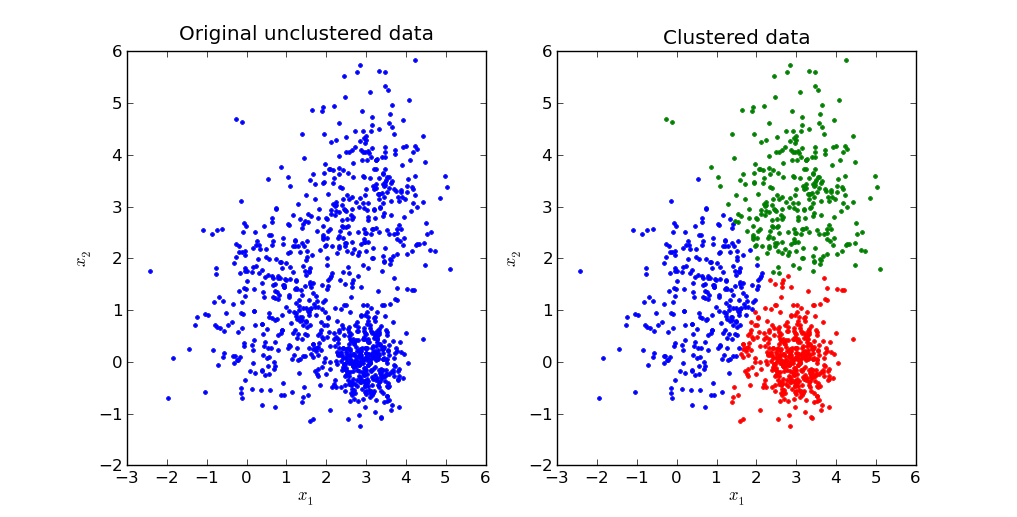
\includegraphics[width=\textwidth]{cluster.png}
\caption{Example of clustering}
\label{fig:ex_clus}
\end{figure}

There are several cluster models, such as connectivity models, centroid models, distribution models, etc. In this work we'll focus on the hierarchical clustering, a connectivity model.

Hierarchical clustering is a method of cluster analysis which builds a hierarchy between its' clusters. There are basically two types of algorithms when talking about hierarchical clusters: the agglomerative and the divisive~\citep{rokach2005clustering}. The main difference between them is that the the agglomerative starts with each elements being it's own cluster and then pairs with another's until all of them are connected (bottom up approach); on the divisive, all elements starts as a unique cluster that are recursively split down into the hierarchy (top down approach).

To define if a set of elements must be clustered, the algorithm base it's decision into an appropriate \textit{metric}. This metric calculates the distance between all elements, and will influence the shape of the clusters, as some elements may be close to one another according to one distance metric and farther away according to another. Table \ref{tab:distances} show some distance metrics.

The \textit{linkage} criteria (\ref{tab:linkage}) determines the distance between clustered sets as a function of the pairwise distances between the elements of each set. If this distance between two clusters is less than some predefined threshold, than those clusters are considered brothers in the hierarchy.

\begin{table}
\begin{center}
\begin{tabular}{cc}
\toprule
\textbf{Distance} & \textbf{Equation}\\
\midrule
Euclidean & $\| u -v \|_{2}$\\[0.3cm]
Correlation & $1 - \dfrac{(u - \bar{u}) \cdot (v-\bar{v})}{\|(u - \bar{u}) \|_{2} \|v-\bar{v} \|_{2}}  $\\[0.3cm] 
Chebyshev & $\max\|u_i-v_i \|$ \\[0.3cm]
Mahalanobis* & $ \sqrt{ (u-v)V^{-1} (u-v)^{T}} $ \\
\bottomrule
\end{tabular}
\caption{Some metrics used for calculate distance between the vector $u$ and $v$. *V is the covariance matrix.}
\label{tab:distances}
\end{center}
\end{table}

\begin{table}
\begin{center}
\begin{tabular}{cc}
\toprule
\textbf{Method} & \textbf{Equation}\\
\midrule
Single & $min(dist(u[i],v[j]))$ \\[0.3cm]
Complete & $ max(dist(u[i],v[j]))$\\[0.3cm]
Centroid & $\|c_s - c_t \|_{2}$ \\[0.3cm]
Average & $ \sum_{ij} \dfrac{d(u[i],v[j])}{(|u| \ast |v|)} $ \\
\bottomrule
\end{tabular}
\caption{Linkage methods used for calculate distance between the clusters $u$ and $v$. $dist(u[i],v[j])$ is the distance between all points $i$ in cluster $u$ and $j$ in cluster $v$. $c_s$ and $c_t$ are the centroids of clusters $s$ and $t$.}
\label{tab:linkage}
\end{center}
\end{table}


\section{Machine Learning and forecasting}

Machine learning is a field of computer science that has the goal to devise complex models and algorithms that can learn from data and lend themselves to prediction. There are several techniques and algorithms inside this field that deals with traditional problems such as classification, regression and clustering. In figure \ref{fig:ml} we have a \textit{machine learning algorithm map}\footnote{source https://machinelearningmastery.com/} with some of the most famous algorithms.

\begin{figure}[!ht]
\centering
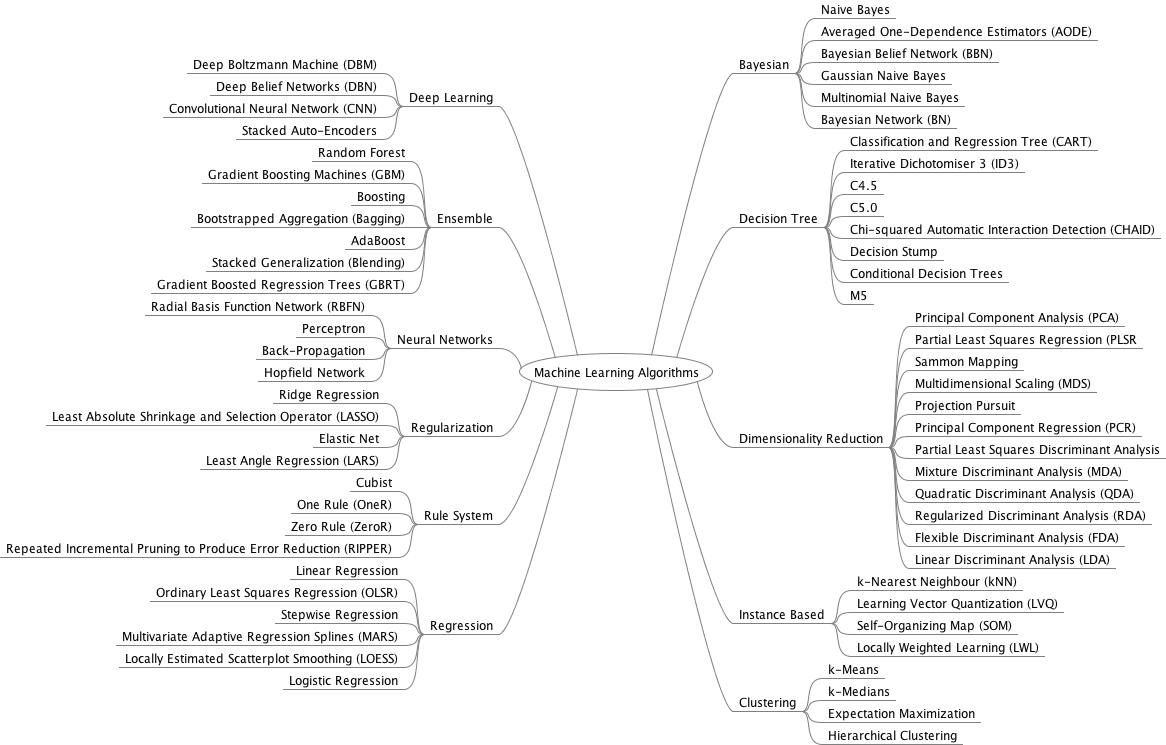
\includegraphics[width=\textwidth]{MachineLearningAlgorithms.png}
\caption{Machine Learning algorithms map}
\label{fig:ml}
\end{figure}

Machine learning techniques can also be useful to forecast problems, as shown in \citet{shen2012stock}, \citet{santillana2015combining} and \citet{bai2005prediction}. 

\todo[inline]{explain why these kind of models are good for forecasting}

In this article we'll approach tree machine learning methods: Random Forest, LASSO and LSTM.

\subsection{Random Forest}

\subsubsection{Decision Trees}

Decision Trees are a type of supervised learning method that builds classification and regression models applying a tree structure. The model learn decision rules that are used to predict the values of the target variable.

The decision tree is created by splitting the dataset into smaller homogeneous subsets and associating them based on some inferred rule. In figure we have an example of this construction.

\begin{figure}
\centering
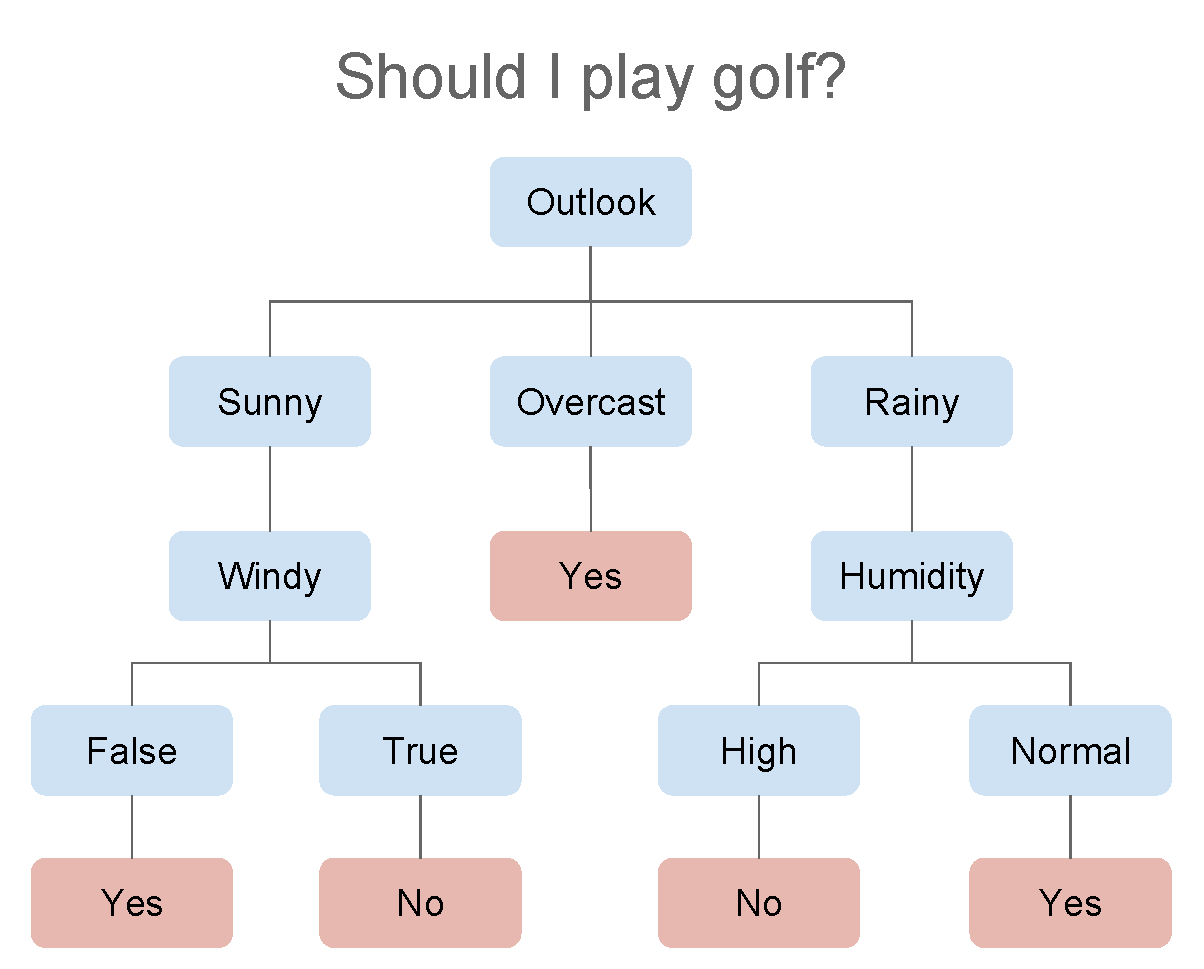
\includegraphics[width=\textwidth/2]{decision_tree.pdf}
\label{fig:decision_tree}
\caption{Decision Tree example}
\end{figure}

Decision Trees are extremely fast and easy to interpret; They perform well on large datasets and can handle numerical and categorical data. The deeper the tree, the more complex the decision rules and the fitter the model. The one big disadvantage of decision trees is that they are prone to overfit.

As deeper the tree is, smaller will become the subsets, which will result in a very accurate model only for the specific training set, that results in a overfitted model. One way to combat this issue is by setting a max depth, this would limit our risk of overfitting; but, this will be at the expense of error due to bias and reduce our predictive quality.

The answer to minimize both error due to bias and error due to variance is to improve our Decision Tree to a Random Forest model.

\subsubsection{Random Forest}

Random Forests (\citet{Breiman2001}) are an learning method for classification and regression build from the ensemble of multiple decision trees. The ability to limit overfitting without substantially increasing error due to bias is what make Random Forest a such powerful method.

The Random Forest algorithm applies a bagging method to the decision trees, which consist in select N random samples with replacement from the training set and fits a modified tree learning algorithm to each one of them.

This modified tree learning algorithm instead of looking through all features in order to select the most optimal split-point, is limited to a random subset of features to choose. This process, usually called \textit{feature bagging}, allows the sub-trees to have a minor correlation between them, which increase the performance of the bagging method once that combining predictions from multiple models in ensembles works better if the predictions from the sub-models are weakly correlated.(add ref)

The number of features p that can be searched at each split point is specified as a parameter to the algorithm. This value can be tune it using cross validation, the default is usually $p/3$ for regression models and $\sqrt{p}$ for classification models.

Given the data $D=\{(X_1,y_1), (X_2,y_2), ... ,(X_n, y_n)\}$, where $X_n$ is the features vector and $y_n$ is the target value, we define $h = \{h(X|\theta_1), h(X|\theta_2), ...,h(X|\theta_k)\}$ as the set of decision trees to ensemble, where $\theta_k$ is the vector of $p$ features randomly chosen. 

Our random forest predictor $f(X)$ is defined by:

$$f(X) = \dfrac{1}{k} \sum_{i=1}^{k} h(X|\theta_i)$$

The uncertainty of the prediction by the standard deviation:

$$\sigma = \sqrt{\dfrac{\sum_{i=1}^{k} (h(X|\theta_i) - f(X))}{k-1}}$$

\subsection{LASSO}
 
 In statistics and machine learning, lasso (least absolute shrinkage and selection operator)
 (also Lasso or LASSO) is a regression analysis method that performs both variable selection and
 regularization in order to enhance the prediction accuracy and interpretability of the statistical
 model it produces. It was introduced by Robert Tibshirani in 1996 based on Leo Breiman’s
 nonnegative garrote.
Given the objective function

\begin{equation}
\dfrac{1}{N} \sum_{i=1}^{N} f(x_i,y_i,\alpha,\beta)
\end{equation}
 
The lasso regularized estimator is the solution of equation \ref{eq:lasso}

\begin{equation}
\min_{\alpha, \beta} \left \{ \dfrac{1}{N} \sum_{i=1}^{N} f(x_i,y_i,\alpha,\beta)  \right \}, \ \ \text{subject to} \ \| \beta \|_{1} \leq t 
\label{eq:lasso}
\end{equation}

\todo[inline]{Add parameters legend}

\subsection{Long-short term memory (LSTM)}

\subsubsection{Artificial Neural Networks}

Artificial Neural Networks (ANN) are collections of connected units called artificial neurons. Each connection between artificial neurons can transmit a signal from one to another, usually this signal is a real number, and the output of each neuron is calculated by a non-linear function of the sum of its inputs.
Those connections have weights that increases or decreases the strength of the signal and are adjusted at the learning process. 

Neurons are organized in layers, each layer may apply a different kind of transformation (activation function) to it's inputs. Figure \ref{fig:ann} show us a example of the structure of a neural network.

\begin{figure}[!ht]
\centering
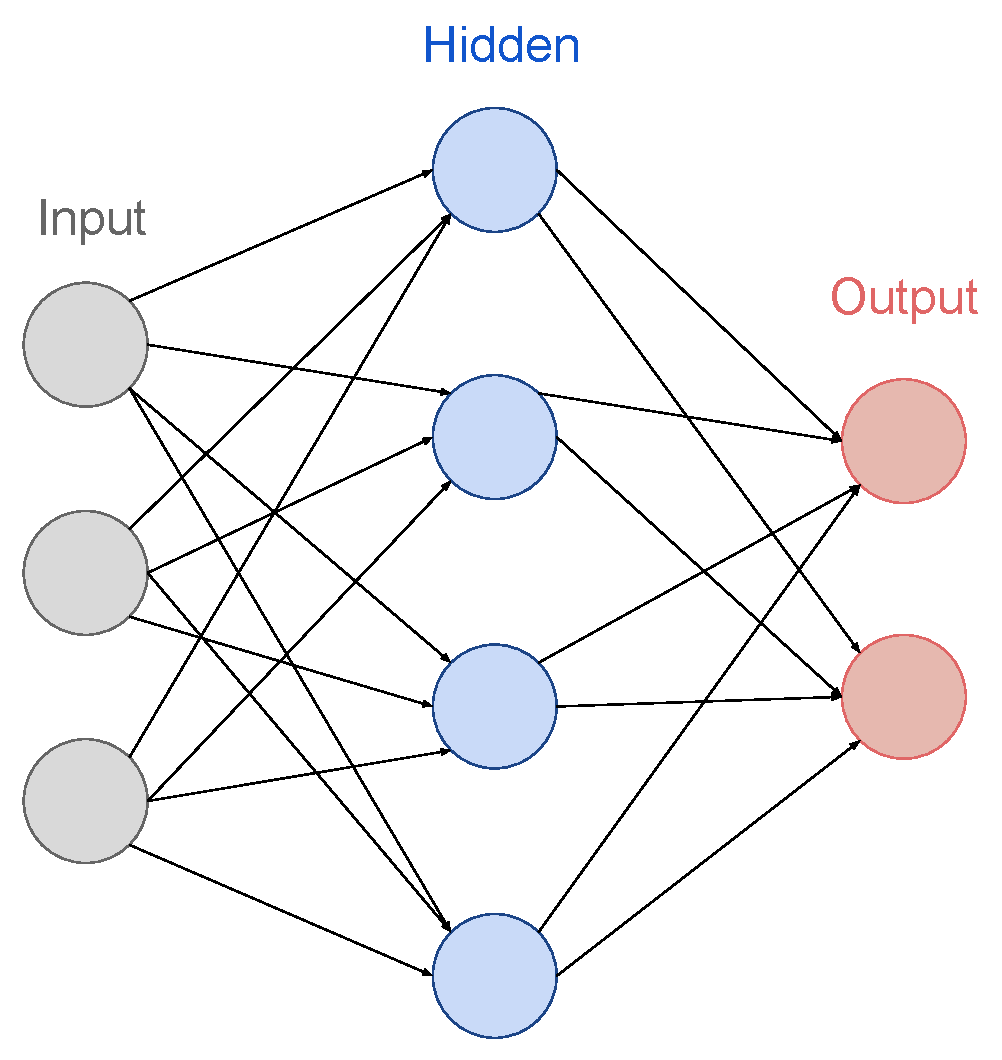
\includegraphics[scale=0.4]{ann.pdf}
\caption{Example of a artificial neural network structure. In this example we have a input layers, one hidden layer and the output layer. Each circle is a neuron.}
\label{fig:ann}
\end{figure}


\subsubsection{Recurrent Neural Networks}

Recurrent neural networks (RNN) are neural networks with loops in them, allowing information to persist. They can be thought of as multiple copies of the same network, each passing a message to a successor. In the figure \ref{fig:rnn} we have the structure of a RNN, where each cell A is the chunk of a neural network,  $x_t$ is the cell input and $h_t$ is the cell output.

\begin{figure}[!ht]
\centering
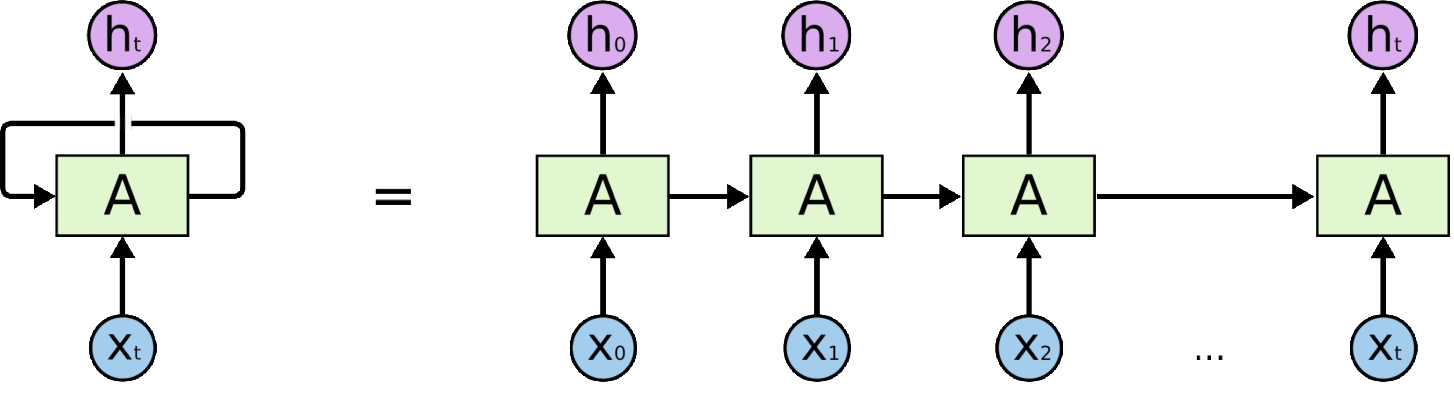
\includegraphics[scale=0.35]{rnn.pdf}
\caption{Example of a unrolled recurrent neural network.}
\label{fig:rnn}
\end{figure}

RNN's learns to use the past information, that means, they remember the information given at time $t_0$ when predicting time $t_\tau$. They usually have great performance when the gap between $t_\tau - t_0$ is small; but they can't handle long-term dependencies. So when $t_\tau - t_0$ is too large, the network become unable to learn to connect the information (which in theory should be able). This problem was extensively explored by \citet{bengio1994learning}.

\subsubsection{Long-short term memory}

Long-short Term Memory Networks (\citet{hochreiter1997long}) are a special kind of RNN, capable of learning long-term dependencies.

\begin{figure}[!h]
\centering
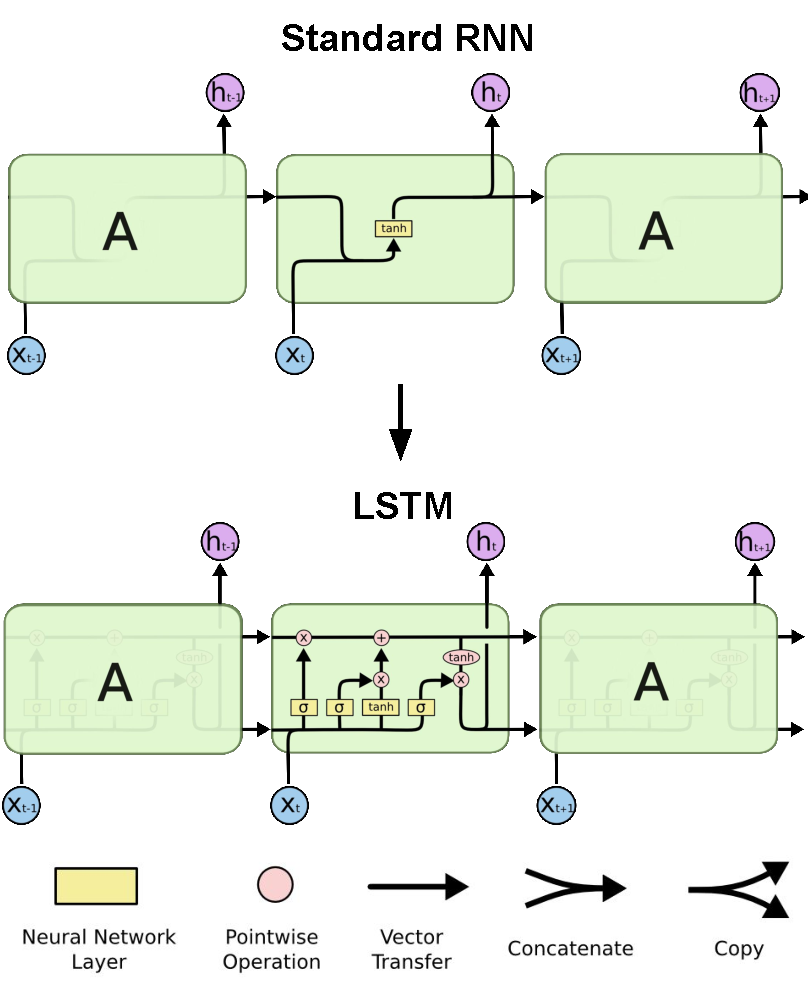
\includegraphics[height=\textheight/2]{lstm1.pdf}
\caption{ala}
\label{fig:lstm1}
\end{figure}

In each cell of chain the network decides which informations to keep and which to forget.

Two important elements from the LSTM cell are the cell state and the gates. The cell state $C_t$, makes possible for information to flow trough the cell unchanged or with some minor interactions.The gates are responsible for those interactions by protecting and controlling the cell state, as shown in \ref{fig:lstm2}.

\begin{figure}[!h]
\centering
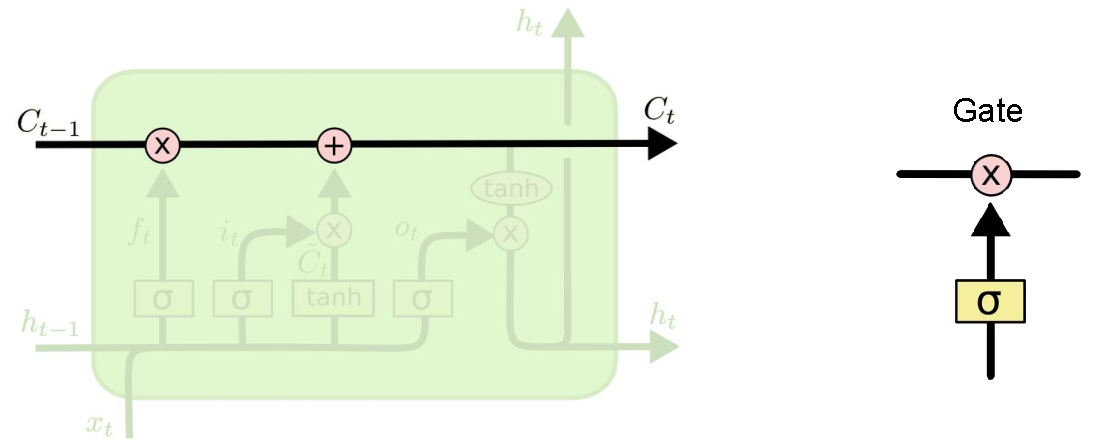
\includegraphics[scale=0.4]{lstm2.pdf}
\caption{Cell state information and gate example}
\label{fig:lstm2}
\end{figure}

Each LSTM cell has 3 gates, composed by a sigmoid neural net layer and a pointwise multiplication operation. The sigmoid layer tell the cell how much information must be kept and how much must go; it have values between 0 and 1 and it is described by the sigmoid function in \ref{eq:sigm}.

\begin{equation}
S(Z) = \dfrac{1}{1+ e^{-z}}
\label{eq:sigm}
\end{equation}

The first gate to pass information to the cell state is the \textit{forget gate layer} which is composed by a sigmoid layer and decides which information to forget from the previous cell state $C_{t-1}$.
It has as input the previous output value $h_{t-1}$ and a new information $x_t$ and output a value $f_t$ between 0 and 1:

\begin{equation}
f_t = \sigma(W_f \cdot [h_{t-1}, xt] + b_f)
\label{eq:ft}
\end{equation}

\begin{figure}[!h]
\centering
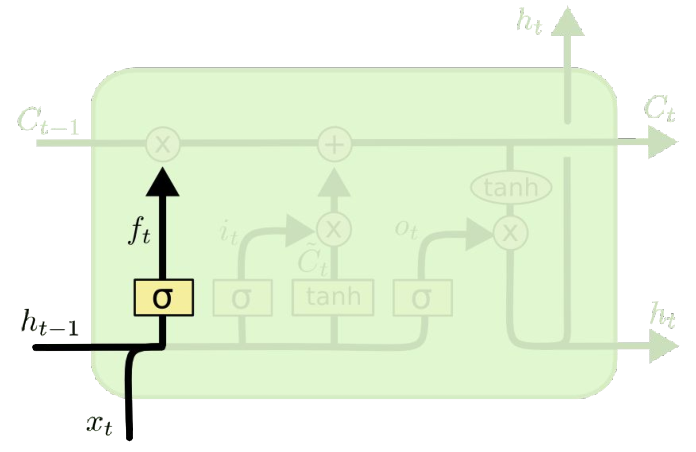
\includegraphics[scale=0.5]{lstm3.pdf}
\caption{LSTM first gate}
\label{fig:lstm3}
\end{figure}

The second gate, is composed by the combination of a sigmoid layer called \textit{input gate layer} and a tanh layer, as shown in figure \ref{fig:lstm4}. This gate decides what new information we'll update to the cell state; The sigmoid layer we'll choose which previous values will be update, and the tanh layer creates the vector $\tilde{C_t}$, which contains the candidate values to be added to the state.

\begin{gather}
i_t = \sigma(W_i \cdot [h_{t-1},x_t] + b_i) \label{eq:it}\\
\tilde{C_t} = tanh(W_c \cdot [h_{t-1},x_t] + b_C) \label{eq:c_tilde}
\end{gather}

\begin{figure}[!ht]
\centering
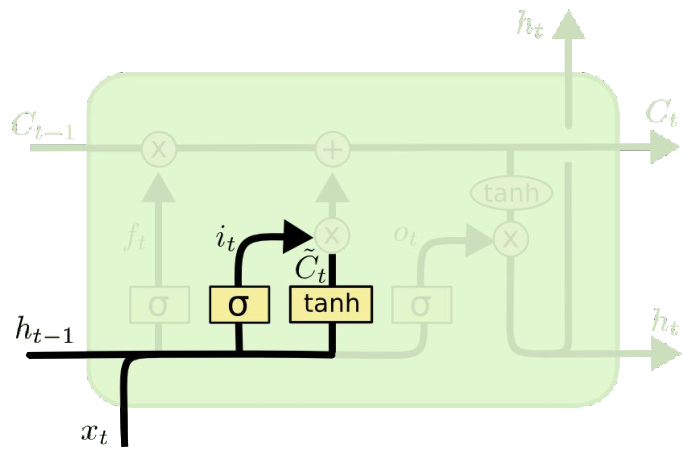
\includegraphics[scale=0.5]{lstm4.pdf}
\caption{LSTM second gate}
\label{fig:lstm4}
\end{figure}


With the equations \ref{eq:ft}, \ref{eq:it} and \ref{eq:c_tilde} defined, we can update the cell state $C_{t-1}$ to $C_t$. The first thing to do is to forget the chosen information $f_t$ by multiplying to $C_{t-1}$. Than we add the combination $i_t * \tilde{C_t}$ which is the new candidate values, scaled by how much we decided to update each state value:

\begin{equation}
C_t = f_t \ast C_{t-1} + i_t \ast \tilde{C_t} 
\label{eq:ct}
\end{equation}

\begin{figure}[!ht]
\centering
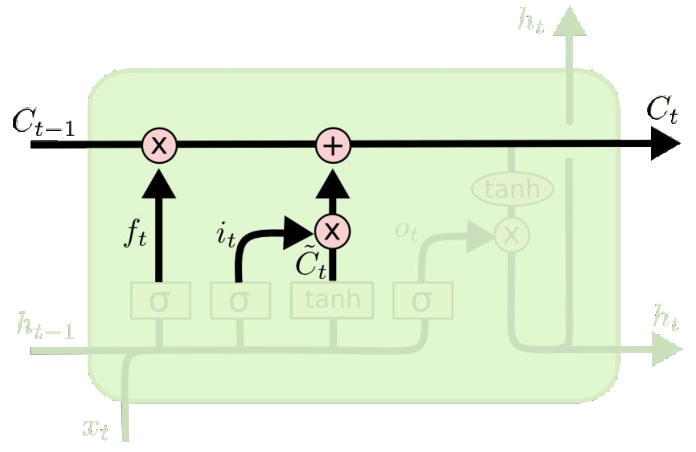
\includegraphics[scale=0.5]{lstm5.pdf}
\caption{Update $C_t$ cell state}
\label{fig:lstm5}
\end{figure}

The third gate defines the output $h_t$ of the cell. We apply a tanh function to the cell state to push the values between -1 and 1, and multiply by the output of a sigmoid layer, which filters the information from the cell state that is interesting for this $h_t$.

\begin{gather}
o_t = \sigma(W_o \cdot [h_{t-1}, x_t] + b_o) \label{eq:ot}\\
h_t = o_t \ast tanh(C_t) \label{eq:ht}
\end{gather}

\begin{figure}[!ht]
\centering
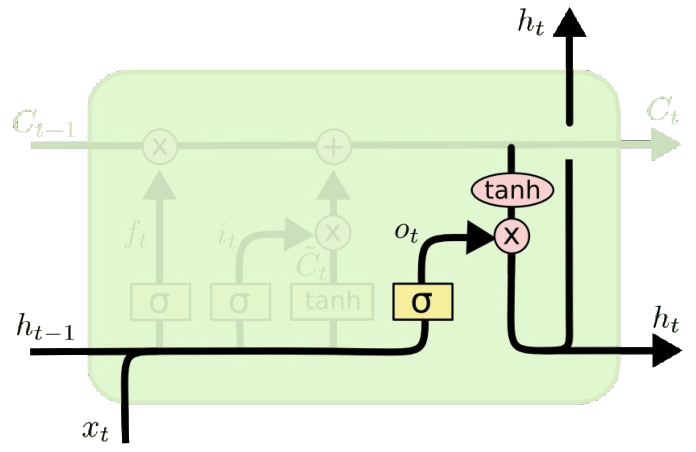
\includegraphics[scale=0.5]{lstm6.pdf}
\caption{output}
\label{fig:lstm6}
\end{figure}

The cells from the LSTM basically receives a previous state and a new input, choose which information to storage for futures outputs, and which information to output in this state.
This makes possible for the LSTM to learn which information to storage.

\newpage	
\chapter{Methodology}

\section{Methodology}


\subsection{Data sources}
The dataset used in the article was provided by the InfoDengue project. 

InfoDengue \citet{codeco2016infodengue} is an integrated dengue alert system, developed as a partnership between Oswaldo Cruz Foundation, Getulio Vargas Foundation and the Ministry of health. As a unique source of carefully curated data for epidemiological studies, InfoDengue monitors 790 cities in Brazil, predicting the weekly number of new cases of dengue in each one of them.

The data consist of the weekly series of dengue incidence,  temperature, humidity, pressure, precipitation intensity, about Dengue in each observed city. It ranges from 2010 until today.

\begin{figure}[h!]
 \centering
 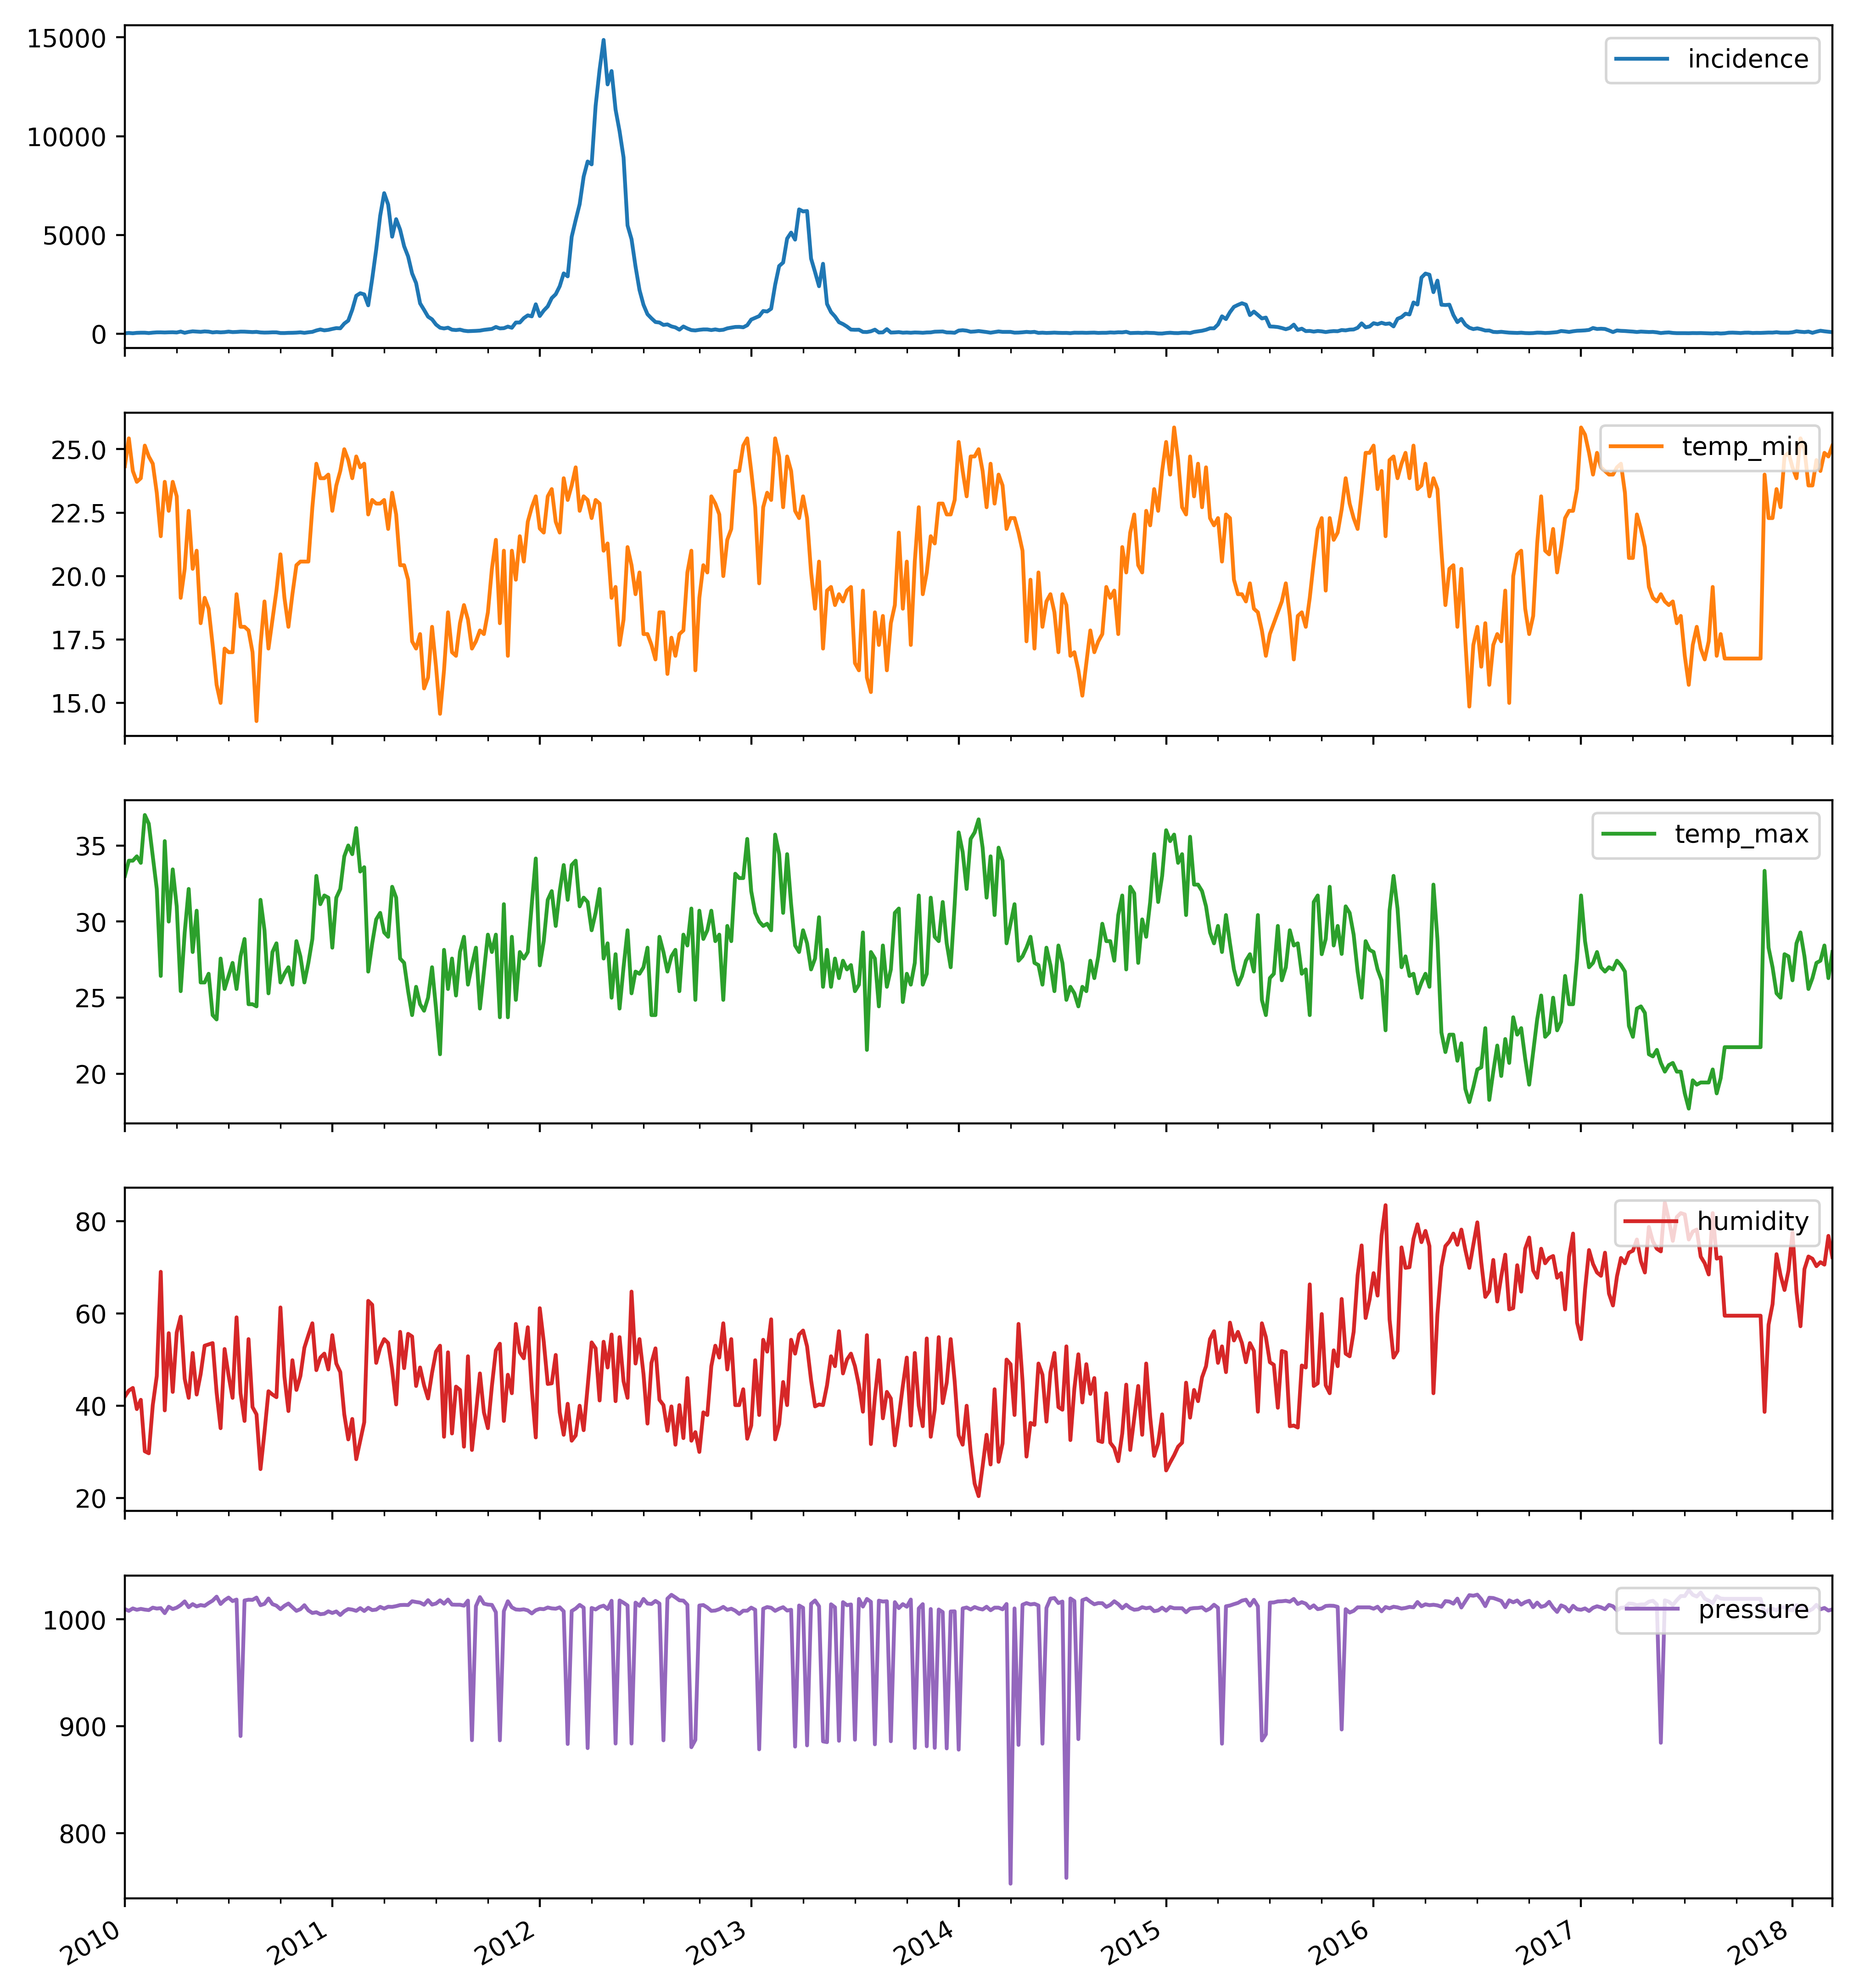
\includegraphics[width=\textwidth]{rio_raw_series.png}
 % rio_raw_series.png: 4000x4000 px, 400dpi, 25.40x25.40 cm, bb=0 0 720 720
 \caption{Time series from Rio de Janeiro features}
 \label{fig: rio_raw}
\end{figure}


\subsection{Data modeling}

It is very difficult to accurately forecast the weekly incidence in a city based only on its historical data. This happens mainly because of the spatial component of disease transmission. Diseases perpetuate themselves by moving from population to population. The flow of individuals between cities is also an important factor.

Dengue is a disease with a clear spatial dependency \citep{stoddard2013house,eisen2009use}. Therefore it makes sense to uses series from neighboring cities nearby in order to reduce uncertainty. Additionally, other cities not necessarily in the vicinity but which display similar historical series of incidence, can also be included as predictors.

\begin{figure}[h!]
 \centering
 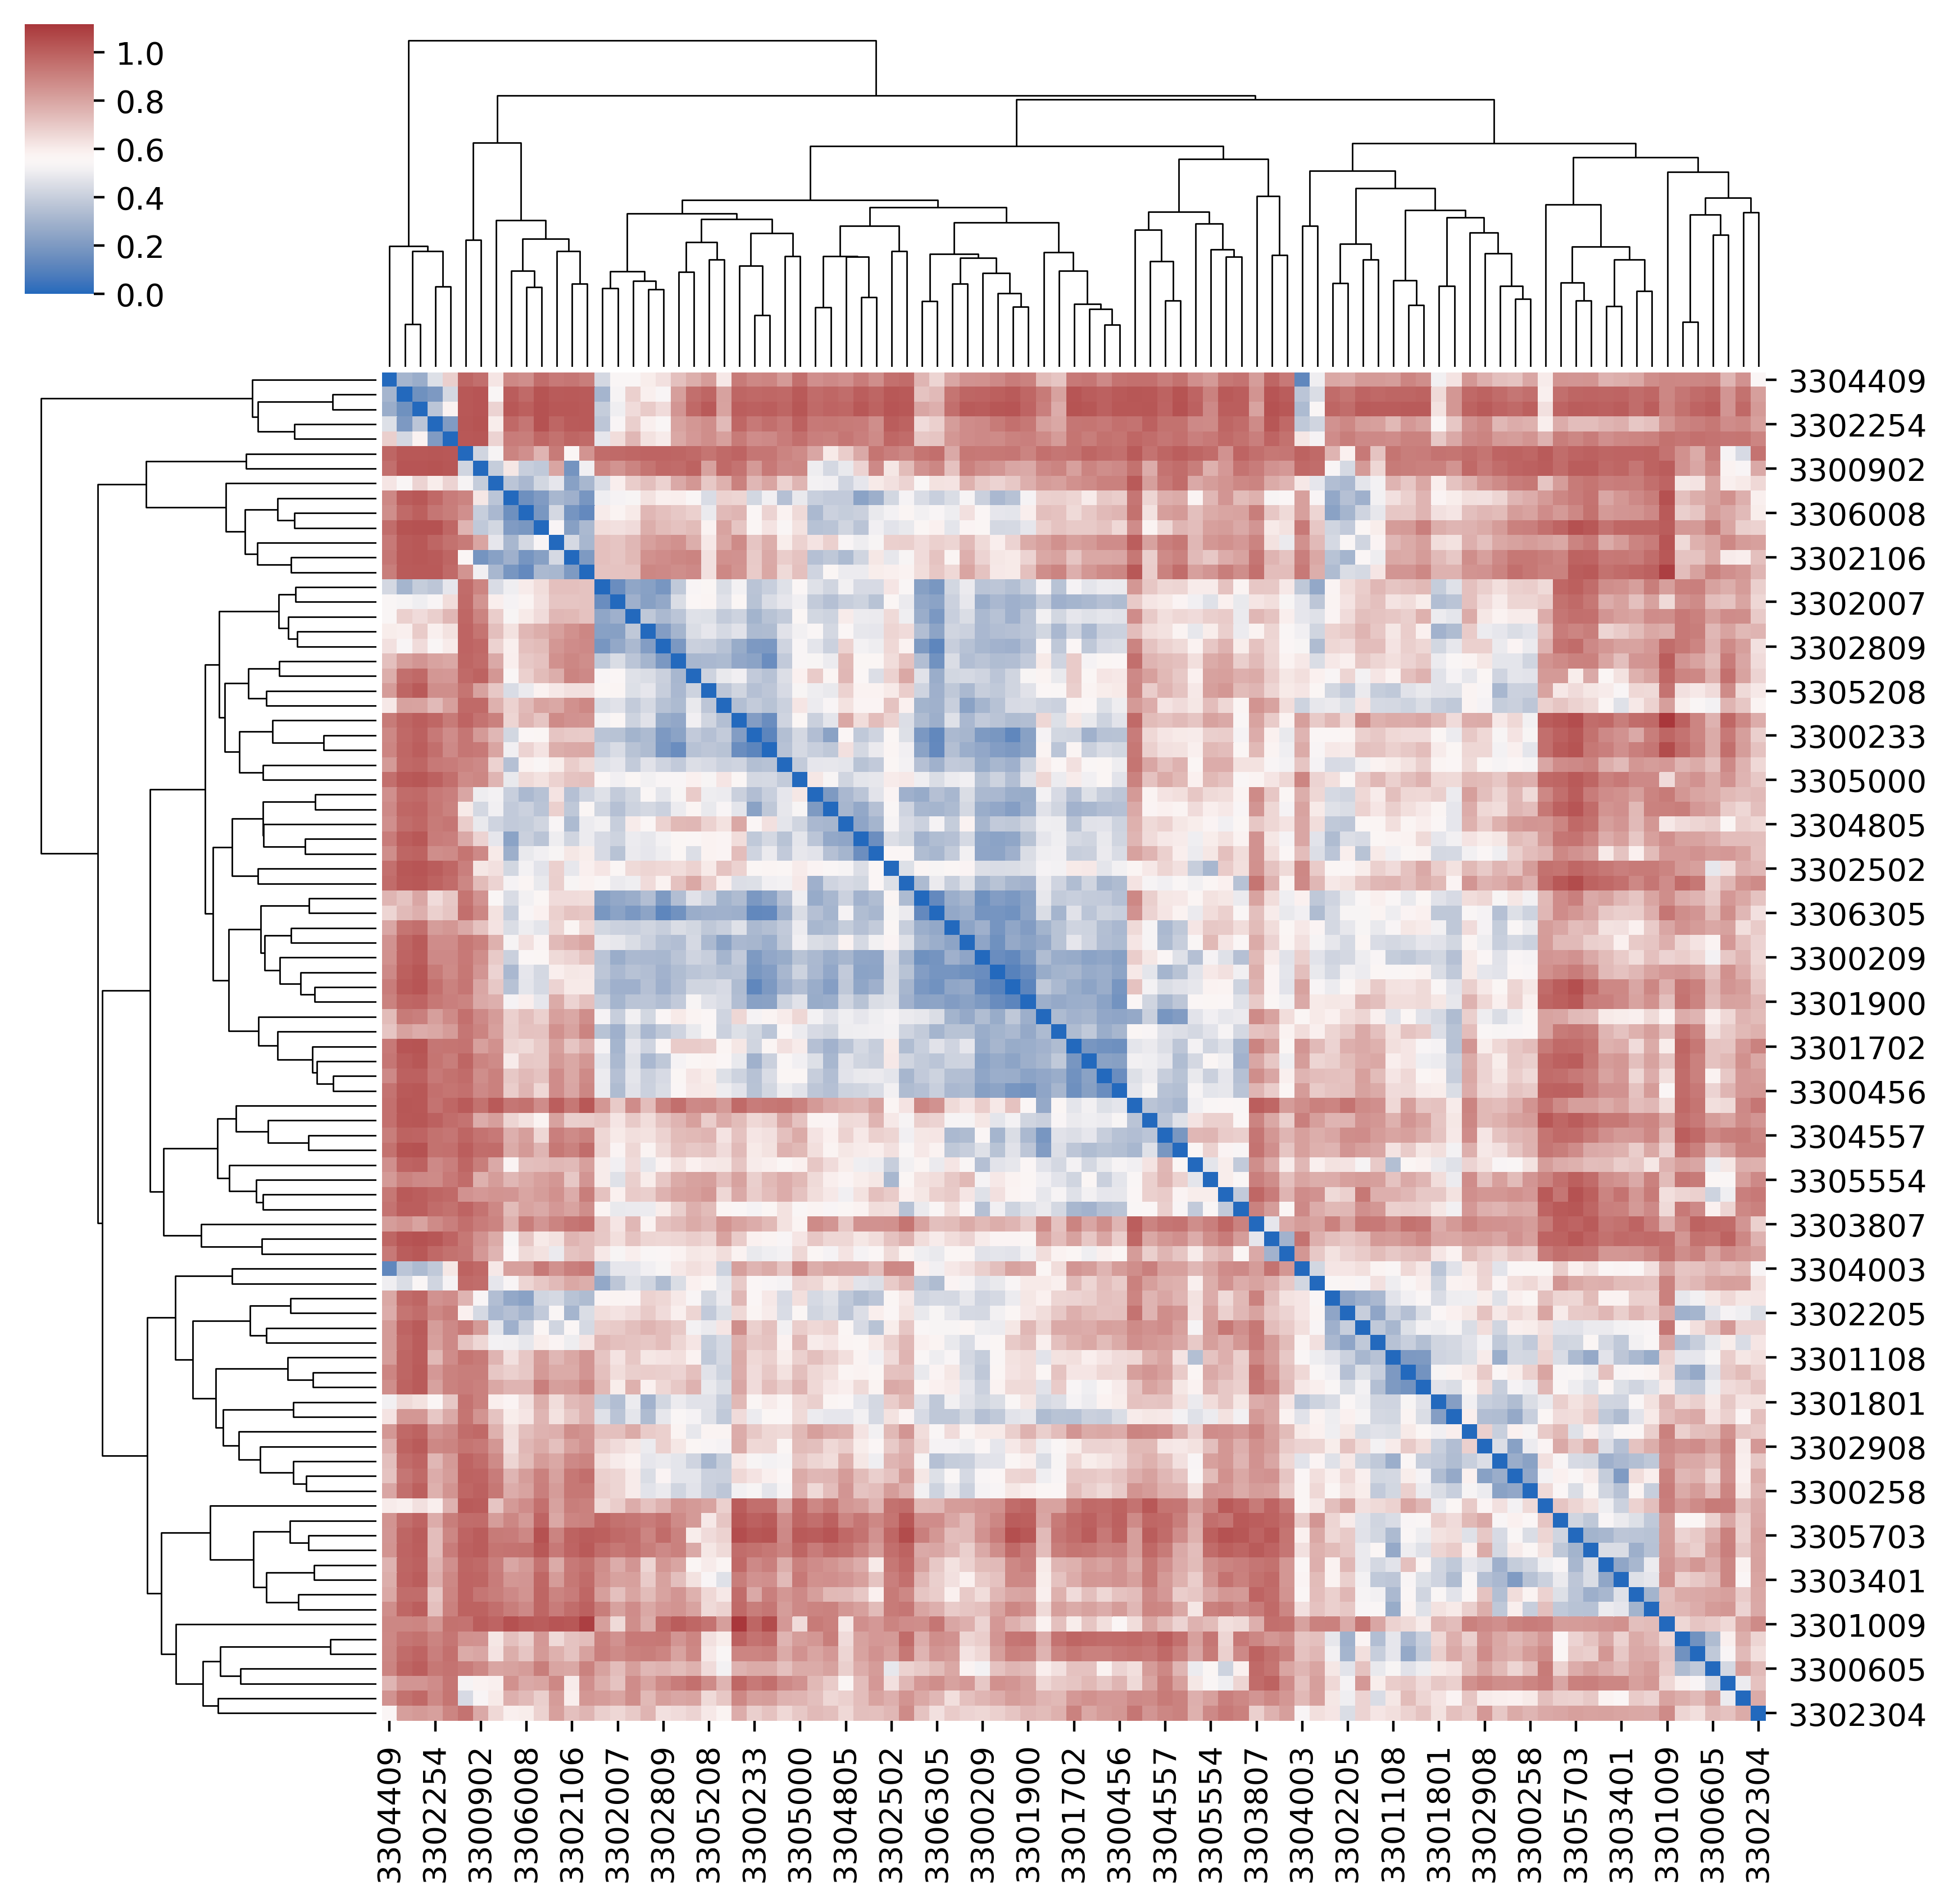
\includegraphics[scale=0.4]{cluster_corr_RJ.png}
 % cluster_corr_RJ.png: 3469x3389 px, 400dpi, 22.03x21.52 cm, bb=0 0 624 610
 \caption{Distance matrix of cities for the state of Rio de Janeiro.}
 \label{fig:corr_rj}
\end{figure}

In order to define the set of cities with relevant predictive information for each city, we clustered all cities within a state based on the correlation distances between incidence time series for each pair of cities. The clusters were calculated applying a  hierarchical agglomerative algorithm, where the distance $d$ of each pair of clusters $(u,v)$ was given by the Farthest Point Algorithm:

$$d(u,v) = max(dist(u[i],v[j])), $$

for all points $i$ in cluster $u$ and $j$ in cluster $v$. The threshold is set to $0.6*max(z))$, where $z$ is the vector of the pairwise correlation distances of the cities. We can see in  \ref{fig:corr_rj} the correlation matrix of the cities from the state of Rio de Janeiro, the threshold defines the distance between the clusters in \ref{fig:cluster_rj}, \ref{fig:cluster_pr}, \ref{fig:cluster_ce}.

For each city, a feature matrix was assembled from the set of time series of each other time series from its cluster.

\begin{figure}[!ht]
\centering
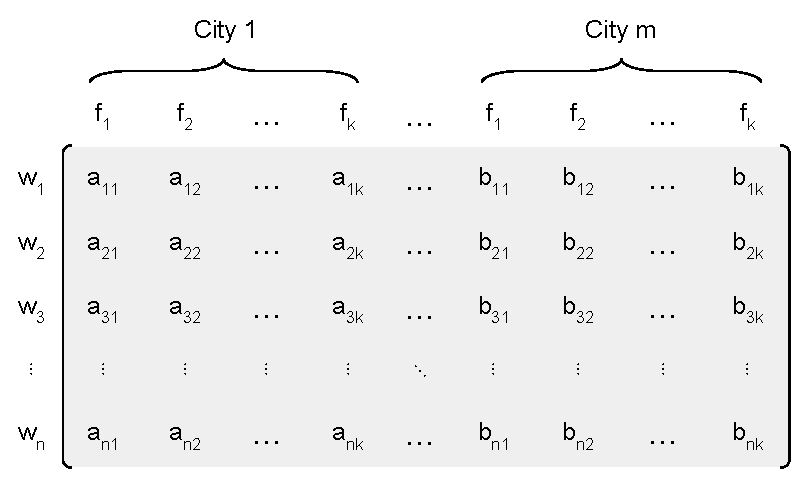
\includegraphics[scale=0.8]{cluster_matrix.pdf}
\caption{Clustered features data with $n$ as the total number of observation, $m$ the total number of cities and $k$ the total number of features for each city.}
\label{fig:m_cluster}
\end{figure}

A single city model was fitted  for a few  cities to serve as a 
baseline against which to compare the effectiveness of the using a cluster of cities as predictors.

\subsection{Forecasting}

We fit tree different classes of models to forecast the incidence timeseries. For all models we adopted a forecast window of 4 weeks, meaning that from any moment in time the model will generate forecasts for the next 4 weeks based only on historical data up to that point.

\begin{description}
 \item \textbf{Random Forest:}
 
 We used a Random Forest regression model to predict a single point in the future based on historical data. In order to turn a time series prediction problem into a regression model, we transformed the series regressors (matrix \ref{fig:m_cluster})into a vector containing not just the last observation of each series but the {\cal D} most recent.

\begin{equation}
y_{t+\tau} = \beta_{t} T_{t}
\label{eq:rf_trans}
\end{equation} 

where t=D,...,n. $T_t$ is defined as $T_t = [X_{t},X_{t-1},...,X_{t-D}]$, where $X_{t-d}$ is the vector with the values of all m predictor series at time $t-d$, where $d=0,...,D$.
$\beta_t$ is a vector $1 x m$ which contains the weights for each value of $T_t$.
The model predicts the incidence at a particular week in the future $y_{t+\tau}$, thus since we wanted to predict 4 weeks into the future, 4 separate models were fitted to data for each $\tau$ varying from 1 to 4.

The figure \ref{fig:rf_matrix} exemplify the data transformation for the input of the model described above:

 \begin{figure}[h!]
 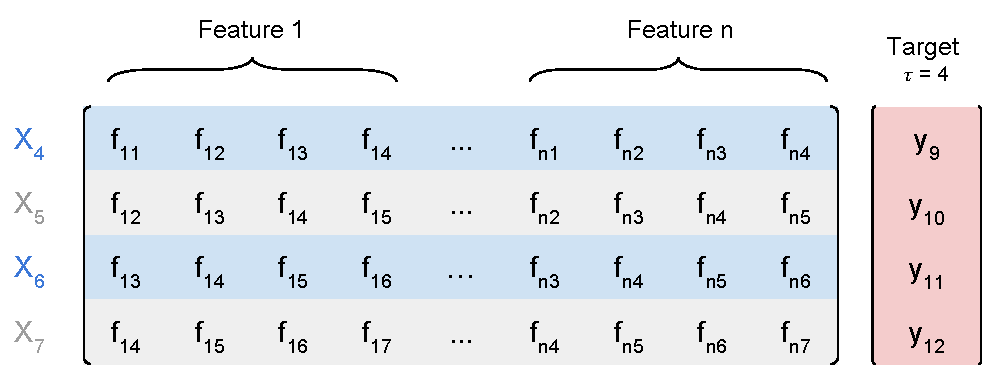
\includegraphics[scale=0.8]{rf_features.pdf}
 % rf_features.pdf: 479x180 px, 72dpi, 16.90x6.35 cm, bb=0 0 479 180
 \caption{Feature matrix transformation for Random Forest input. The first matrix is the original data, where $a_{ij}$ is the feature $i$ at time $j$, $j=[1,..,n]$, and $y_i$ is the incidence of dengue cases at time $i$, $i=[1,...,n]$. In this example, $D=4$ and $\tau=4$, so our first vector is $T_4$, which contains all m predictors series at times $(t_1,t_2,t_3,t_4)$, and our target is $y_{t+\tau} = y_{D+\tau} = y_{8}$. The last input must contain the last target, therefore $y_{t+\tau} = y_n$ and $T_t = T_{n-4}$.}
 \label{fig:rf_matrix}
\end{figure}

 \item \textbf{Long short term memory (LSTM)}
 
 A LSTM model is a recurrent deep neural network model developed to handle predictions of timeseries. We used a LSTM model with topology given in table \ref{tab:lstm}. The model was trained for 100 epochs with a look back of 4 weeks and a forecasting window of also 4 weeks. \todo{aqui não indica o número de hidden layers, etc}
The loss function used was the MSLE defined in equation (\ref{eq:msle}), where $y, \hat{y}$ are the true and predicted value, respectively:

\begin{equation}
MSLE = \dfrac{1}{n} \sum_{i=1}^{i=n} (log(y_i +1) - log(\hat{y}_i +1))^{2}
\label{eq:msle}
\end{equation}

\begin{table}
\begin{center}
\begin{tabular}{cccc}
  \textbf{Layer} & \textbf{Output} & \textbf{Activation} & \textbf{Dropout}\\
  \hline
  LSTM  & (1,4,4) & tanh & 0.2 \\
  LSTM  & (1,4,4) & tanh & 0.2\\
  LSTM  & (1,4) & tanh & 0.2\\
  Dense & (1,4) & relu & - \\
  \hline
\end{tabular}
\caption{Parameters used to build LSTM model}
\label{tab:lstm}
\end{center}
\end{table}

The feature matrix used to train the LSTM needs to be a 3 dimensional matrix, where each 'slice' is a temporal window from our features regressors (\ref{fig:m_cluster}). The first dimension of the matrix is the features, therefore has size equal to $k$; the second dimension is the number of samples that the model will use to train (total number observations - (look back + forecasting window)); the third dimension is the temporal windows cut observed (look back + forecasting window).

The figure \ref{fig:lstm_matrix} exemplifies the construction of this matrix when forecasting window = 4 and look back = 4.

\begin{figure}[!h]
\centering
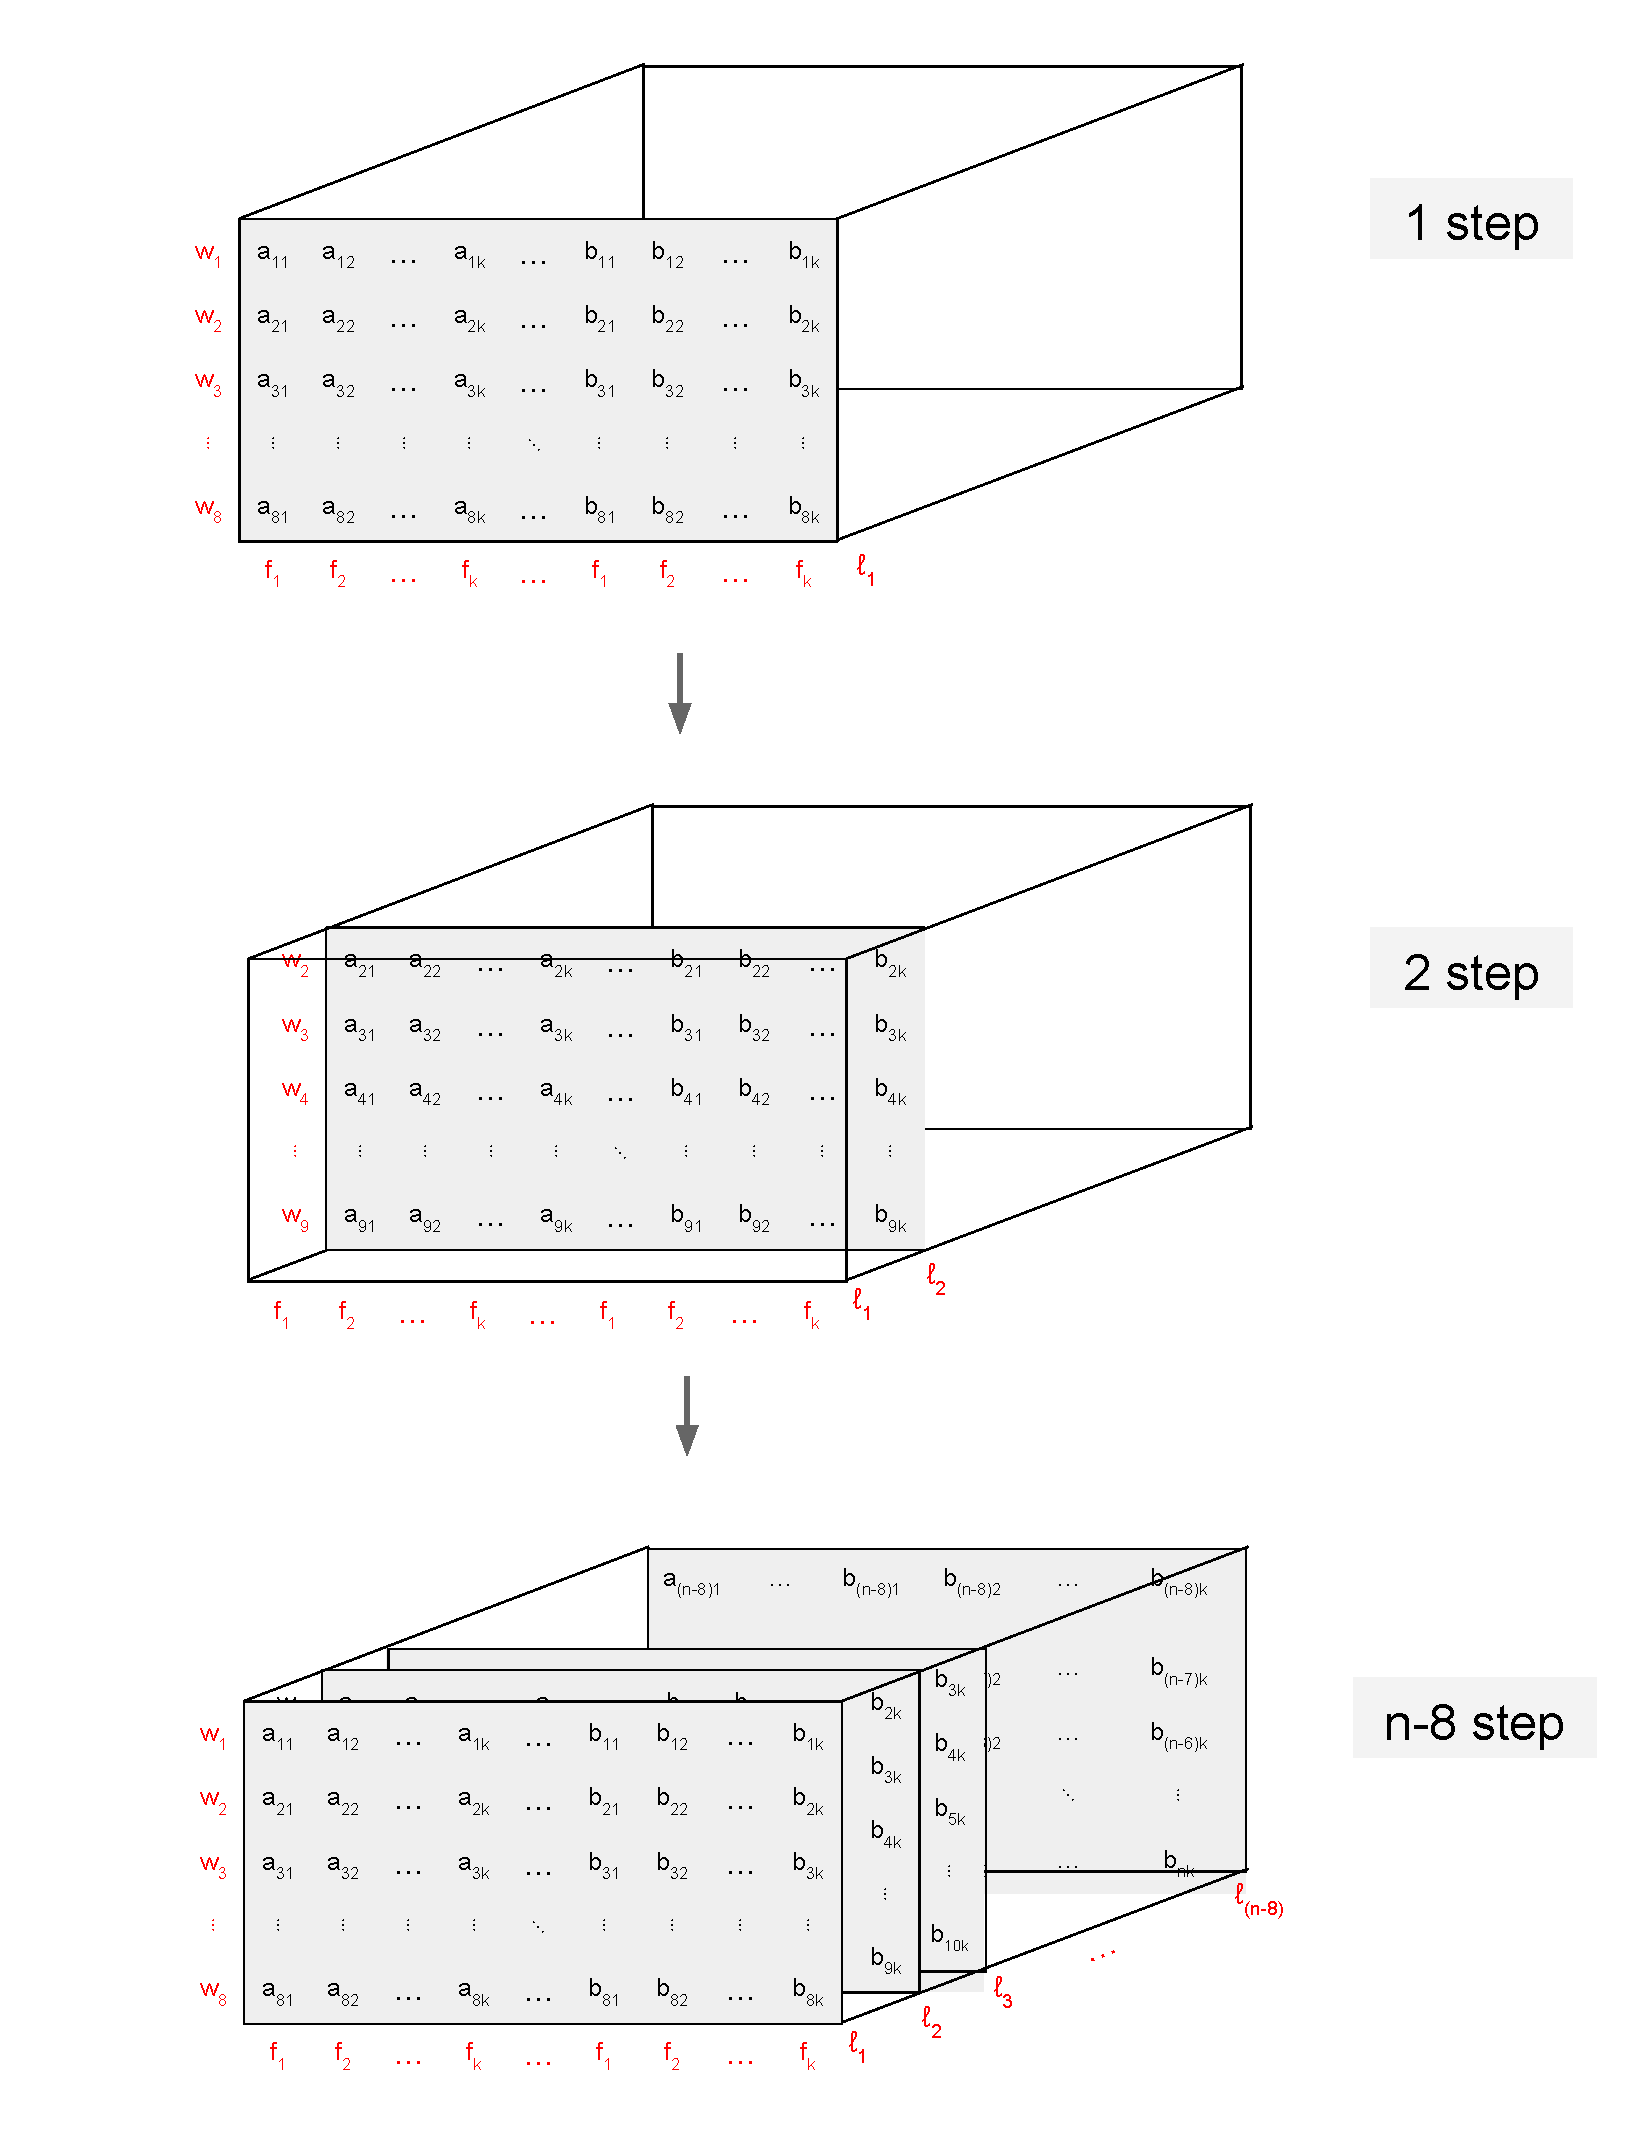
\includegraphics[width = \textwidth]{lstm_matrix.pdf}
\caption{Creation of features matrix used to train the LSTM model.}
\label{fig:lstm_matrix}
\end{figure}

 \item \textbf{Lasso regression}
 
  A Lasso model is an estimator for linear regression models which also performs variable selection as it can estimate sparse coefficient matrices. 
  
  We fitted a cross-validation Lasso model using the Least Angle Regression (LARS) defined by \citet{efron2004least}; Additionally, we applied an evolutionary tree-based optimization procedure proposed by \citet{olson2016evaluation} to define the best parameters.
  
    The feature matrix used was the same used by the Random Forest model (figure \ref{fig:rf_matrix}).
  
\end{description}


\section{Results}
\label{results}

\subsection{Cluster analysis}

We performed the clustering of cities as described above for every state in the Infodengue dataset. Figure \ref{fig:cluster_cf} shows the incidence series for a few clusters for Rio de Janeiro state of the entire historical period available. We can see that cities clustered together display similar incidence patterns. Depictions of the remaining clusters can be found in the supplementary material. Cluster sizes are variable, the mean size of clusters for each state can be seen in table \ref{tab:clusters_size}.

\begin{table}
\begin{center}
\begin{tabular}{lccc}
  & \textbf{Number of cities} & \textbf{Number of Clusters} & \textbf{Cluster mean size}\\
 \hline
 \textbf{Rio de Janeiro} & 92 & 14 & 6\\
 \textbf{Paraná} & 399 & 54 & 6 \\
 \textbf{Ceará} & 184 & 49 & 3 \\
 \hline
\end{tabular}
\label{tab:clusters_size}
\caption{Clusters results comparison between states.}
\end{center}
\end{table}

\begin{figure}[h!]
 \centering
 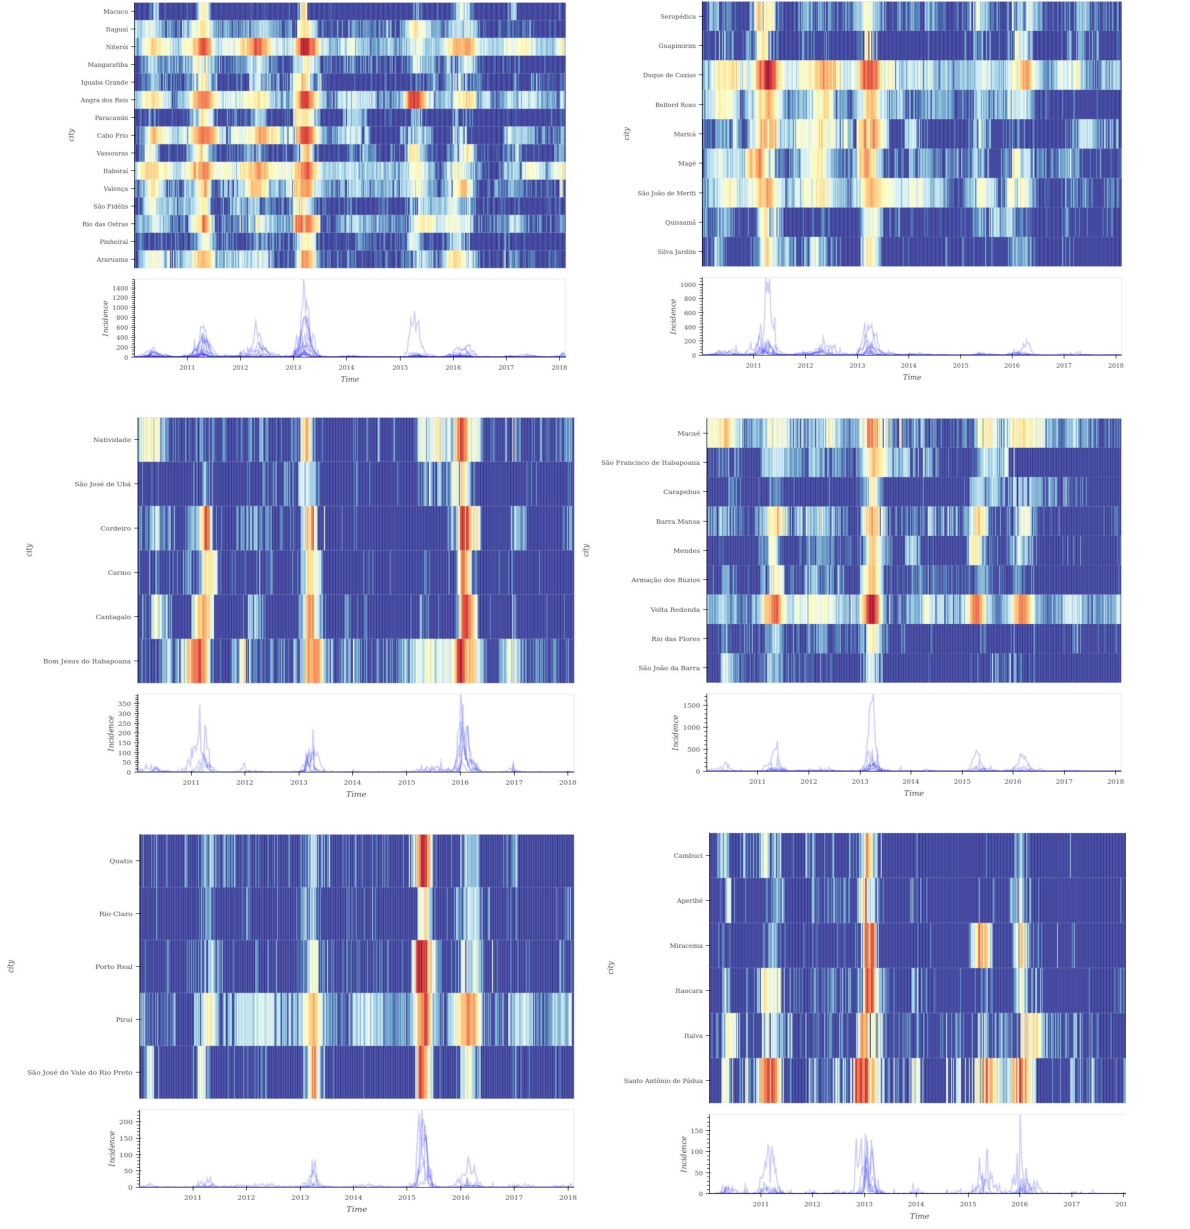
\includegraphics[scale=0.8]{./clusters_rj_holo.pdf}
 \caption{dengue incidence for some clusters from Rio de Janeiro state.}
 \label{fig:cluster_cf}
\end{figure}


The cluster found within each state are shown in figures \ref{fig:cluster_rj}, \ref{fig:cluster_ce}, \ref{fig:cluster_pr}. They can also be seen in the map in figures xxx.

\begin{figure}[h!]
 \centering
 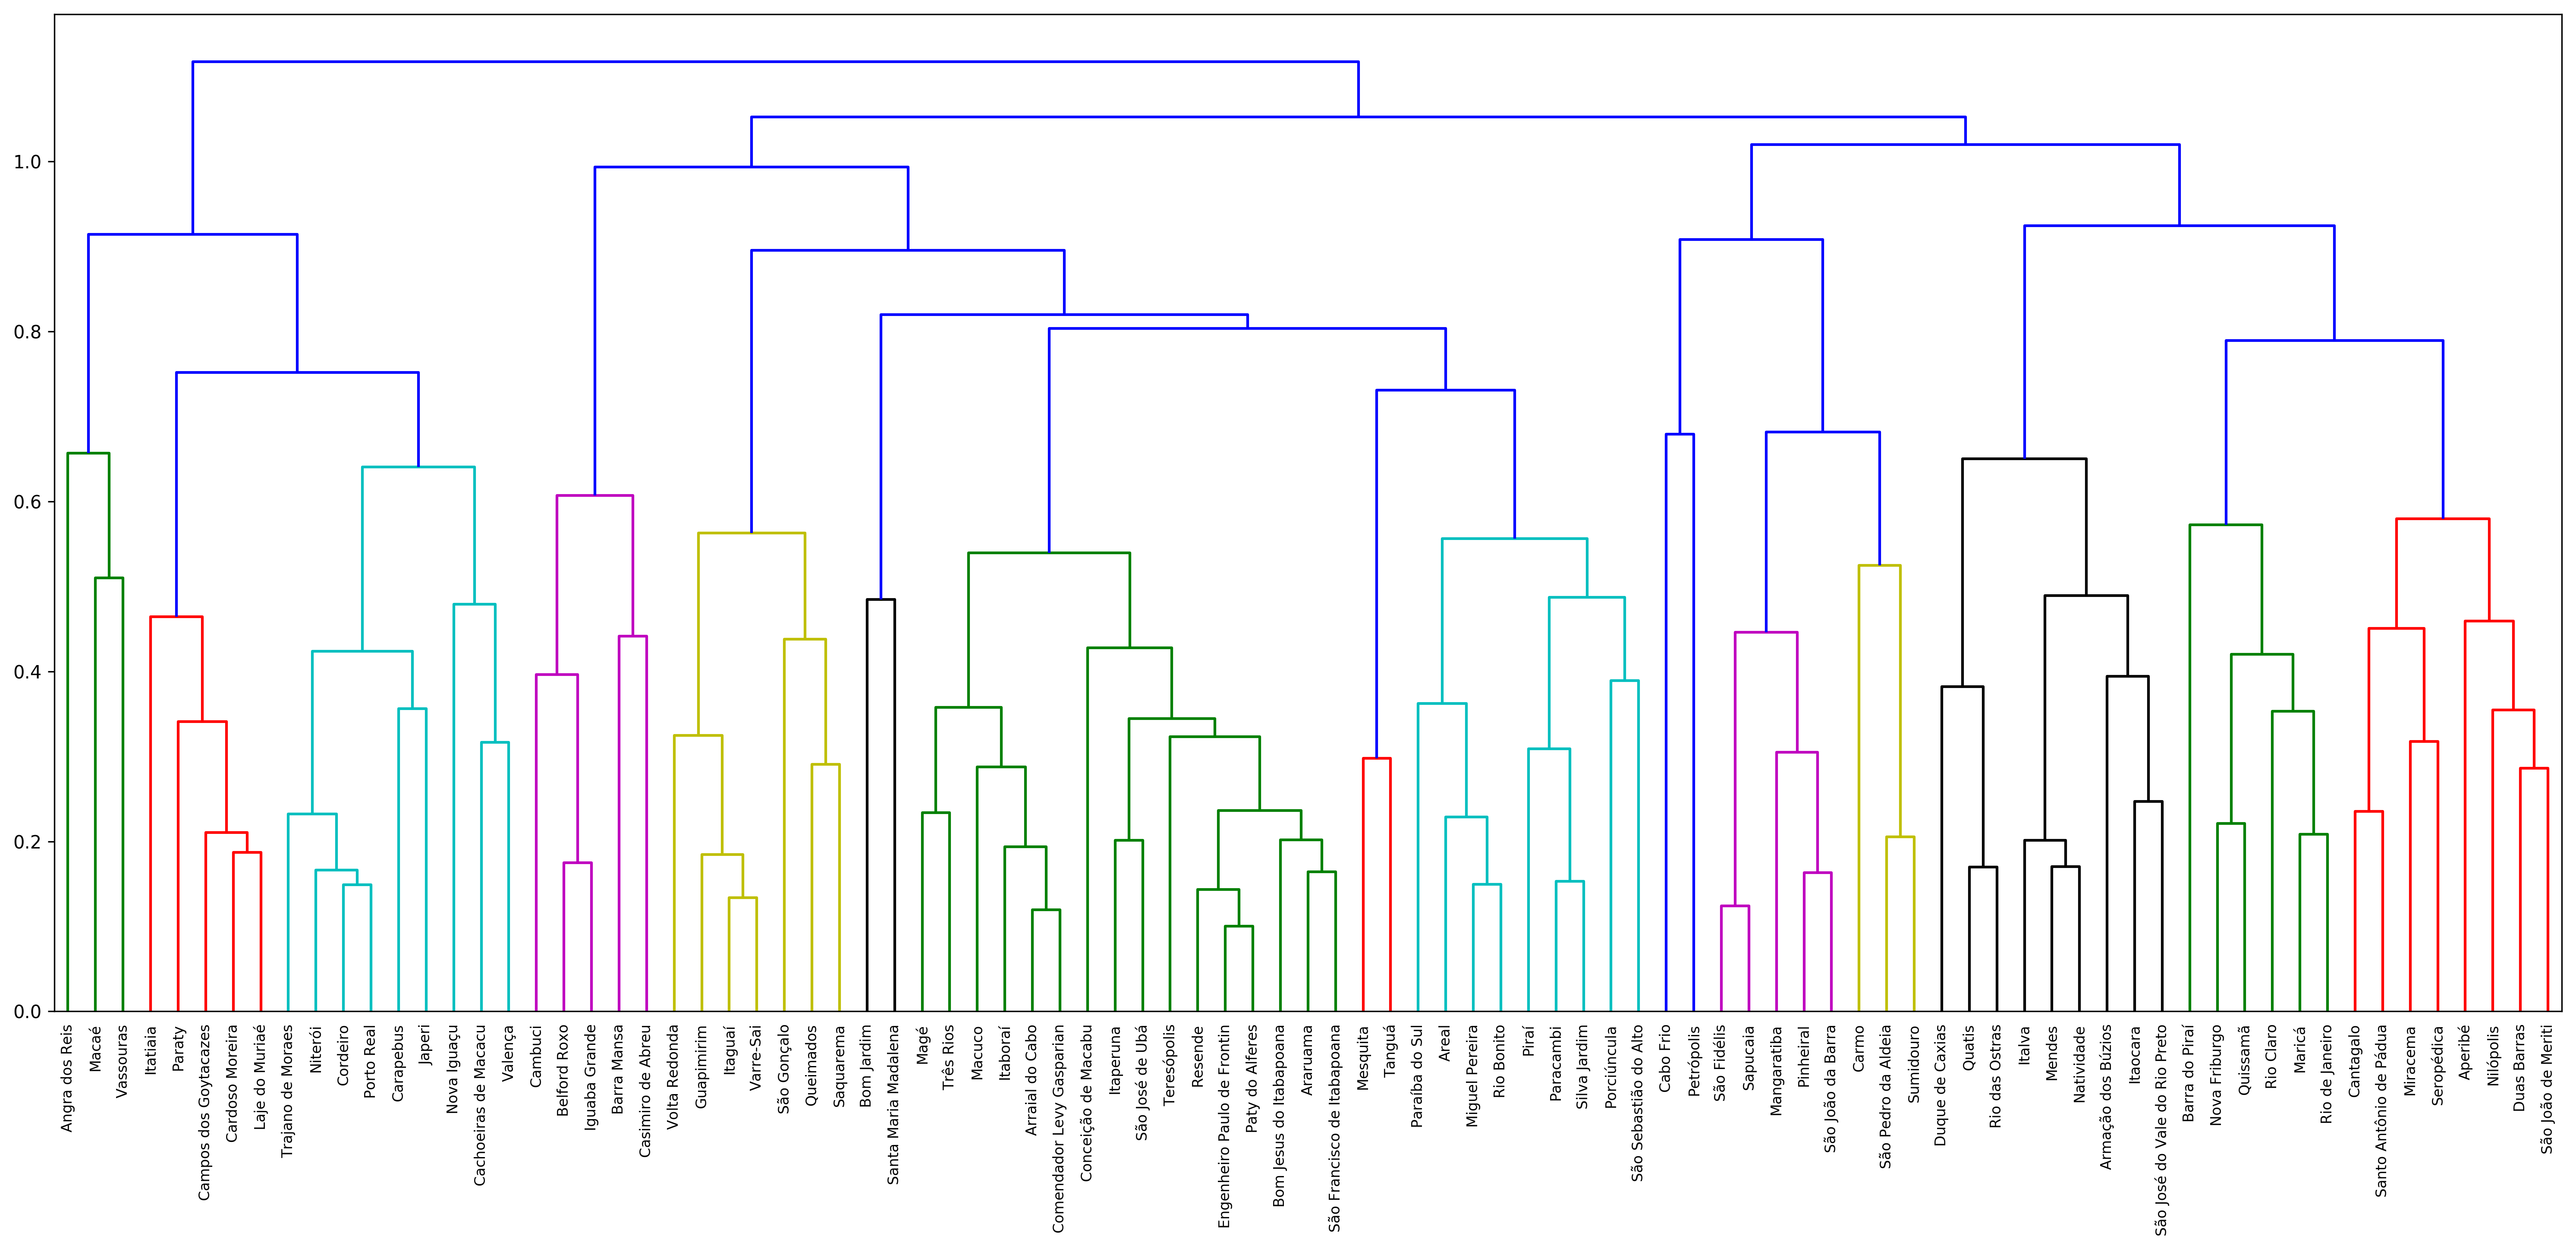
\includegraphics[height=\textheight]{clusterRJ_06.png}
 % clusterRJ_0.6.png: 5971x2894 px, 300dpi, 50.55x24.50 cm, bb=0 0 1433 695
 \caption{Hierarchical cluster of Rio de Janeiro.}
 \label{fig:cluster_rj}
\end{figure}


\subsection{Forecasting}
We measured the performance of the forecasting models by the magnitude of the prediction error for week $t+4$ where $t$ is the last week observed. The prediction errors were calculated as mean squared error (MSE), and mean squared log error(MSLE).

We trained the lasso and random forest models for the single features data, that means, without the features series from it's clusters. In figure \ref{fig:cluster_compar_rj} we compared the losses out-of-sample for each type of input data. We
can see that, in general, the models with cluster data have less error variance than the single models.

\begin{figure}[!ht]
\centering
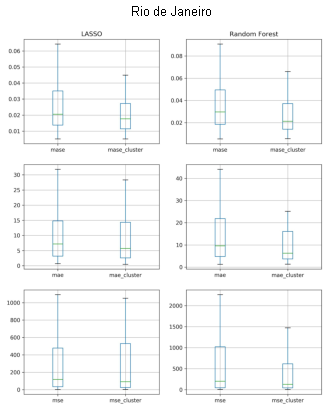
\includegraphics[width=\textwidth]{cluster_model_compar_RJ.pdf}
\caption{Loss comparison between models trained with and without cluster features for Rio de Janeiro state.}
\label{fig:cluster_compar_rj}
\end{figure}

\begin{figure}[!ht]
\centering
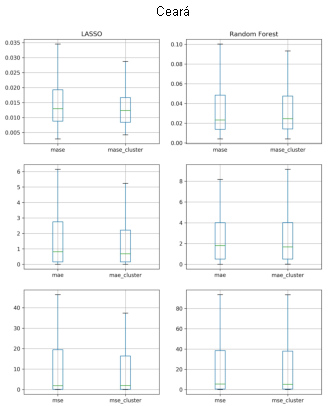
\includegraphics[width=\textwidth]{cluster_model_compar_CE.pdf}
\caption{Loss comparison between models trained with and without cluster features for Ceará state.}
\label{fig:cluster_compar_ce}
\end{figure}

\begin{figure}[!ht]
\centering
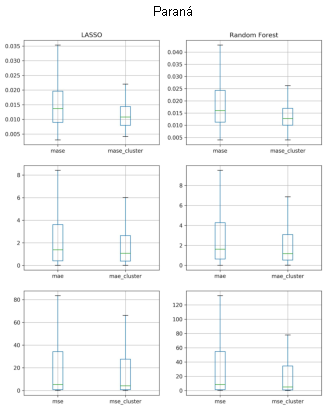
\includegraphics[width=\textwidth]{cluster_model_compar_PR.pdf}
\caption{Loss comparison between models trained with and without cluster features for Paraná state.}
\label{fig:cluster_compar_pr}
\end{figure}

The comparison between the models efficiency is showed at figure \ref{fig:losses_heat} for each state separately. The LSTM models returned minor error than the LASSO and Random Forest when looking at the MASE and MSE losses for all the states. It is interesting to notice that the LASSO model have performed better than the Random Forest for the state of Rio de Janeiro, but in Paraná and Ceará it had a lower performance than the Random Forest.

\begin{figure}[!ht]
\centering
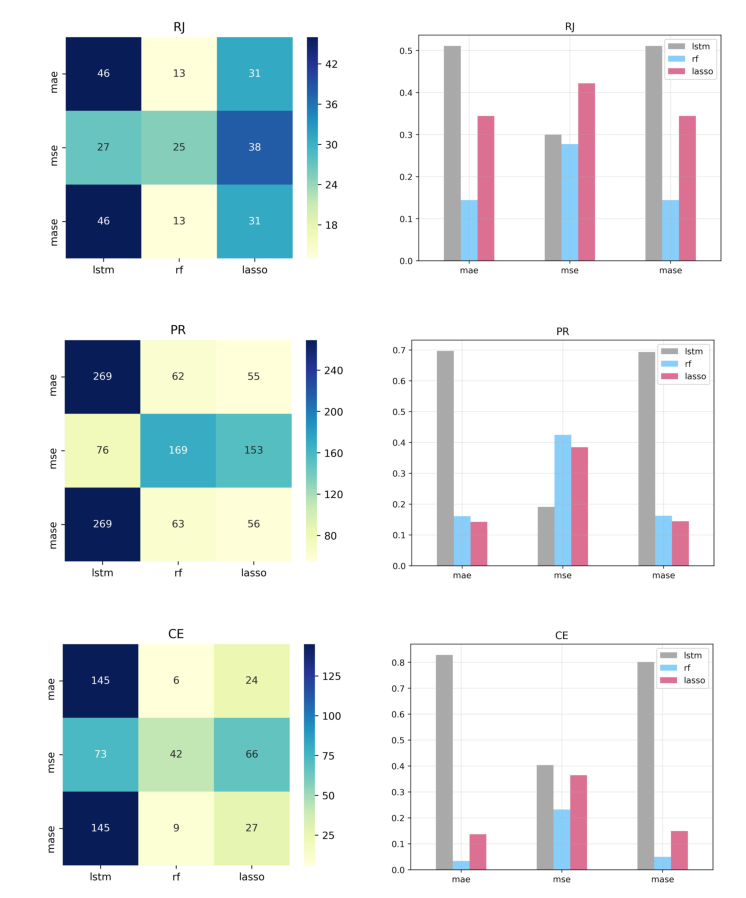
\includegraphics[width=\textwidth]{loss_count.pdf}
\caption{The left column contains the heatmap matrix for each state with the count of times that a specific model performed better for each type of loss. The right column contains the percentage bar plot where of 'winning' performance for each loss.} 
\label{fig:losses_heat}
\end{figure}
\todo[inline]{winning?}

We calculated the qqplot (ref) for each state with the goal to understand if the predicted value belongs to the empirical distribution of the data. 

Figures xx and yy show the performance of the prediction  both \emph{in-sample} and  \emph{out-of-sample}, for some cities in the states of Rio de Janeiro, Paraná and Ceará. The full cities predictions are in the appendices section.

\todo[inline]{add figure prediction some cities - escolher}

\newpage
\chapter{Conclusions and Final Considerations}
The model has show good performance for both large and small cities from various parts of Brasil. This shows that the set of predictor series selected is capable to characterize the epidemic dynamics.

The extra information provided by the sister cities' series allowed the model to substantially outperform the base model. The LSTM model was capable of consistently predict the incidence pattern of non-epidemic years. 

Despite the fact that the LSTM model didn't reach the peak of the epidemics, it showed consistency when predicting the start of the epidemic, which is the most valuable information when forecasting epidemics.

Random Forest and Lasso models showed good results but when comparing out of sample predictions it didn't showed consistency as the lstm model.

It's interesting to look to those cities and learn which model performs better and made a ensemble into those models.

The LSTM model have the tendency of underestimate the epidemics which is good when thinking of resources cost for the state public health.

Machine and deep learning are increasing areas with a lot of potential to forecast, outstanding classical forecasting models.

LSTM have great potential and space for derivate models as pointed by ref and ref, which can lead to a specific models for epidemics forecasting in future works.

It's important to remember that lstm has a high computational cost which can make random forest and lasso better option depending of the case?



\newpage
\phantomsection
\addcontentsline{toc}{chapter}{References}
\bibliographystyle{model1-num-names}
\bibliography{sample}

\newpage
\phantomsection
\addcontentsline{toc}{chapter}{Appendices}
\chapter*{Appendices}

\scriptsize
\begin{center}
\begin{longtable}{l g g g b b b g g g}
\caption{Losses of Rio de Janeiro}\\
3301207 & 6.2 & \textcolor{pink}{3.1e+02} & 0.021 & 6.7 & 3.7e+02 & 0.023 & \textcolor{pink}{6.2} & 5.4e+02 & \textcolor{pink}{0.021}\\ 
3300605 & \textcolor{pink}{1.8e+01} & \textcolor{pink}{1.7e+03} & \textcolor{pink}{0.016} & 1.8e+01 & 2.1e+03 & 0.017 & 2.3e+01 & 4.3e+03 & 0.021\\ 
3301108 & 1.3e+01 & 1e+03 & 0.024 & \textcolor{pink}{1.3e+01} & \textcolor{pink}{1e+03} & \textcolor{pink}{0.024} & 1.4e+01 & 1.9e+03 & 0.027\\ 
3301504 & \textcolor{pink}{1.3e+01} & \textcolor{pink}{1.3e+03} & \textcolor{pink}{0.01} & 1.4e+01 & 2e+03 & 0.011 & 1.6e+01 & 2.7e+03 & 0.012\\ 
3303104 & 1.2e+01 & 1.1e+03 & 0.012 & \textcolor{pink}{1.2e+01} & \textcolor{pink}{1.1e+03} & \textcolor{pink}{0.012} & 1.3e+01 & 1.6e+03 & 0.013\\ 
3305133 & 4.1 & 7.2e+01 & 0.021 & \textcolor{pink}{4.1} & \textcolor{pink}{7.2e+01} & \textcolor{pink}{0.021} & 3.1 & 7.6e+01 & 0.015\\ 
3301009 & 5.1e+01 & 3.4e+03 & 0.026 & \textcolor{pink}{5.1e+01} & \textcolor{pink}{3.4e+03} & \textcolor{pink}{0.026} & 2.9e+01 & 2.8e+03 & 0.015\\ 
3304706 & 1.7e+01 & 5.4e+02 & 0.021 & 9.0 & \textcolor{pink}{5.4e+02} & 0.011 & \textcolor{pink}{1.7e+01} & 5.3e+02 & \textcolor{pink}{0.021}\\ 
3303203 & 5.9 & 1.2e+02 & 0.021 & 6.3 & \textcolor{pink}{1.2e+02} & 0.022 & \textcolor{pink}{5.9} & 1.5e+02 & \textcolor{pink}{0.021}\\ 
3303500 & \textcolor{pink}{1.6e+01} & \textcolor{pink}{4.7e+02} & \textcolor{pink}{0.013} & 3.4e+01 & 2.1e+03 & 0.029 & 2e+01 & 9.2e+02 & 0.017\\ 
3304557 & 3.2e+02 & 4.5e+05 & 0.031 & \textcolor{pink}{3.2e+02} & \textcolor{pink}{4.5e+05} & \textcolor{pink}{0.031} & 3.6e+02 & 6.2e+05 & 0.034\\ 
3304144 & 3.9 & 2.6e+01 & 0.032 & 2.8 & 1e+01 & 0.023 & \textcolor{pink}{3.9} & \textcolor{pink}{2.6e+01} & \textcolor{pink}{0.032}\\ 
3302858 & 6.9 & 1.7e+02 & 0.022 & \textcolor{pink}{6.9} & \textcolor{pink}{1.7e+02} & \textcolor{pink}{0.022} & 9.4 & 2.2e+02 & 0.03\\ 
3306206 & 1.1e+01 & 2.1e+02 & 0.026 & \textcolor{pink}{1.1e+01} & \textcolor{pink}{2.1e+02} & \textcolor{pink}{0.026} & 8.5 & 5.3e+02 & 0.02\\ 
3300100 & 2.3e+01 & 1.5e+03 & 0.023 & \textcolor{pink}{2.3e+01} & \textcolor{pink}{1.5e+03} & \textcolor{pink}{0.023} & 3.5e+01 & 6.1e+03 & 0.035\\ 
3300209 & \textcolor{pink}{1e+01} & \textcolor{pink}{2.9e+02} & \textcolor{pink}{0.019} & 1.6e+01 & 5e+02 & 0.03 & 1.1e+01 & 4.2e+02 & 0.02\\ 
3300704 & 2.2e+01 & 1.2e+03 & 0.05 & 2e+01 & \textcolor{pink}{1.2e+03} & 0.045 & \textcolor{pink}{2.2e+01} & 6.3e+02 & \textcolor{pink}{0.05}\\ 
3301876 & 6.7 & 6.9e+01 & 0.023 & 3.2 & 3.8e+01 & 0.011 & \textcolor{pink}{6.7} & \textcolor{pink}{6.9e+01} & \textcolor{pink}{0.023}\\ 
3301900 & \textcolor{pink}{2.1e+01} & \textcolor{pink}{9.5e+02} & \textcolor{pink}{0.014} & 3.6e+01 & 2.3e+03 & 0.024 & 4.4e+01 & 8e+03 & 0.029\\ 
3302007 & 5.7 & 5.5e+01 & 0.025 & \textcolor{pink}{5.7} & \textcolor{pink}{5.5e+01} & \textcolor{pink}{0.025} & 1.1e+01 & 4.3e+02 & 0.048\\ 
3302452 & 4.2 & 3.8e+01 & 0.025 & 2.4 & \textcolor{pink}{3.8e+01} & 0.014 & \textcolor{pink}{4.2} & 3.7e+01 & \textcolor{pink}{0.025}\\ 
3302601 & 4.6 & 2.8e+01 & 0.019 & 4.3 & 2.7e+01 & 0.018 & \textcolor{pink}{4.6} & \textcolor{pink}{2.8e+01} & \textcolor{pink}{0.019}\\ 
3303302 & 3.5e+01 & 3.1e+03 & 0.021 & \textcolor{pink}{3.5e+01} & \textcolor{pink}{3.1e+03} & \textcolor{pink}{0.021} & 5.3e+01 & 1e+04 & 0.032\\ 
3303609 & 1.1e+01 & 1.5e+02 & 0.19 & 4.8 & 3.1e+01 & 0.086 & \textcolor{pink}{1.1e+01} & \textcolor{pink}{1.5e+02} & \textcolor{pink}{0.19}\\ 
3303955 & 2.0 & \textcolor{pink}{1.4e+01} & 0.012 & \textcolor{pink}{2.0} & 1.5e+01 & \textcolor{pink}{0.012} & 2.9 & 6.1e+01 & 0.017\\ 
3304524 & 2.2e+01 & 6.2e+02 & 0.042 & 1.7e+01 & 3.7e+02 & 0.032 & \textcolor{pink}{2.2e+01} & \textcolor{pink}{6.2e+02} & \textcolor{pink}{0.042}\\ 
3304805 & 7.2 & 8.4e+01 & 0.027 & 6.8 & 6.4e+01 & 0.025 & \textcolor{pink}{7.2} & \textcolor{pink}{8.4e+01} & \textcolor{pink}{0.027}\\ 
3306107 & 1.6e+01 & 7.5e+02 & 0.02 & 2.1e+01 & 9.7e+02 & 0.026 & \textcolor{pink}{1.6e+01} & \textcolor{pink}{7.5e+02} & \textcolor{pink}{0.02}\\ 
3300456 & 8.1 & 1.1e+02 & 0.04 & \textcolor{pink}{8.1} & \textcolor{pink}{1.1e+02} & \textcolor{pink}{0.04} & 1.2e+01 & 2.5e+02 & 0.059\\ 
3301702 & 2.3e+01 & 1.3e+03 & 0.019 & \textcolor{pink}{2.3e+01} & \textcolor{pink}{1.3e+03} & \textcolor{pink}{0.019} & 3.3e+01 & 4.5e+03 & 0.028\\ 
3301850 & 3.5 & \textcolor{pink}{5.1e+01} & 0.013 & 6.4e+10 & 2.6e+23 & 2.3e+08 & \textcolor{pink}{3.5} & 6.7e+01 & \textcolor{pink}{0.013}\\ 
3302502 & 1.6e+01 & 4.1e+02 & 0.045 & 4.5e+11 & 1.3e+25 & 1.3e+09 & \textcolor{pink}{1.6e+01} & \textcolor{pink}{4.1e+02} & \textcolor{pink}{0.045}\\ 
3302700 & 9.4 & 1.8e+02 & 0.039 & 1.4e+01 & 2.3e+02 & 0.056 & \textcolor{pink}{9.4} & \textcolor{pink}{1.8e+02} & \textcolor{pink}{0.039}\\ 
3304151 & 3.2 & 1.3e+01 & 0.039 & 2.1 & \textcolor{pink}{1.3e+01} & 0.026 & \textcolor{pink}{3.2} & 1.2e+01 & \textcolor{pink}{0.039}\\ 
3305554 & 3.5 & 3.1e+01 & 0.013 & \textcolor{pink}{3.5} & \textcolor{pink}{3.1e+01} & \textcolor{pink}{0.013} & 2.7 & 3.1e+01 & 0.01\\ 
3305109 & \textcolor{pink}{1.2e+01} & \textcolor{pink}{1.7e+02} & \textcolor{pink}{0.029} & 1.5e+11 & 1.4e+24 & 3.7e+08 & 1.7e+01 & 6.7e+02 & 0.043\\ 
3305604 & 6.1 & 5e+01 & 0.094 & \textcolor{pink}{6.1} & \textcolor{pink}{5e+01} & \textcolor{pink}{0.094} & 6.7 & 2.9e+02 & 0.1\\ 
3302304 & 1.8 & 5.1 & 0.029 & 0.8 & \textcolor{pink}{5.1} & 0.013 & \textcolor{pink}{1.8} & 3.4 & \textcolor{pink}{0.029}\\ 
3303807 & 1.6e+01 & 3.7e+02 & 0.078 & 1.2e+01 & 1.6e+02 & 0.056 & \textcolor{pink}{1.6e+01} & \textcolor{pink}{3.7e+02} & \textcolor{pink}{0.078}\\ 
3300258 & \textcolor{pink}{7.1} & \textcolor{pink}{4.2e+02} & \textcolor{pink}{0.0088} & 7.7 & 5.3e+02 & 0.0095 & 9.9 & 8.5e+02 & 0.012\\ 
3303708 & 6.3 & \textcolor{pink}{2.4e+02} & 0.011 & 6.4 & 3.3e+02 & 0.011 & \textcolor{pink}{6.3} & 4e+02 & \textcolor{pink}{0.011}\\ 
3303856 & 3.4 & \textcolor{pink}{6e+01} & 0.015 & \textcolor{pink}{3.4} & 8.8e+01 & \textcolor{pink}{0.015} & 3.4 & 1.2e+02 & 0.015\\ 
3304904 & \textcolor{pink}{8.1e+01} & \textcolor{pink}{1.2e+04} & \textcolor{pink}{0.016} & 9e+11 & 4.8e+25 & 1.8e+08 & 8.4e+01 & 2.6e+04 & 0.017\\ 
3305505 & 1.9e+01 & 1e+03 & 0.0095 & \textcolor{pink}{1.9e+01} & \textcolor{pink}{1e+03} & \textcolor{pink}{0.0095} & 2.7e+01 & 1.9e+03 & 0.013\\ 
3305208 & 2.3e+01 & 7.6e+02 & 0.041 & \textcolor{pink}{2.3e+01} & \textcolor{pink}{7.6e+02} & \textcolor{pink}{0.041} & 9.3 & 4.3e+02 & 0.017\\ 
3301306 & 4.1 & 4.2e+01 & 0.015 & \textcolor{pink}{4.1} & \textcolor{pink}{4.2e+01} & \textcolor{pink}{0.015} & 3.8 & 3.1e+01 & 0.013\\ 
3305752 & 3.4 & 2e+01 & 0.025 & \textcolor{pink}{3.4} & \textcolor{pink}{2e+01} & \textcolor{pink}{0.025} & 5.2 & 3.2e+02 & 0.038\\ 
3300233 & 3.7e+01 & 1.8e+03 & 1.5 & 5.1 & 8.6e+01 & 0.2 & \textcolor{pink}{3.7e+01} & \textcolor{pink}{1.8e+03} & \textcolor{pink}{1.5}\\ 
3300407 & 1.3e+01 & 5.4e+02 & 0.04 & 9.8 & 1.1e+02 & 0.03 & \textcolor{pink}{1.3e+01} & \textcolor{pink}{5.4e+02} & \textcolor{pink}{0.04}\\ 
3300936 & 2.3 & 1.2e+01 & 0.0099 & \textcolor{pink}{2.3} & \textcolor{pink}{1.2e+01} & \textcolor{pink}{0.0099} & 2.1 & 1.4e+01 & 0.0087\\ 
3302809 & 8.3 & 9.6e+01 & 0.055 & \textcolor{pink}{8.3} & \textcolor{pink}{9.6e+01} & \textcolor{pink}{0.055} & 3.8 & 2.1e+02 & 0.025\\ 
3304508 & 2.0 & \textcolor{pink}{5.2} & 0.049 & 1.2 & 5.5 & 0.029 & \textcolor{pink}{2.0} & 5.4 & \textcolor{pink}{0.049}\\ 
3304755 & 4.5 & 4.1e+01 & 0.046 & 5.3 & 8.1e+01 & 0.055 & \textcolor{pink}{4.5} & \textcolor{pink}{4.1e+01} & \textcolor{pink}{0.046}\\ 
3305000 & 6.1 & 4.3e+01 & 0.11 & 1.5 & \textcolor{pink}{4.3e+01} & 0.028 & \textcolor{pink}{6.1} & 1.2e+01 & \textcolor{pink}{0.11}\\ 
3302403 & 2.1e+01 & 5.9e+02 & 0.016 & \textcolor{pink}{2.1e+01} & \textcolor{pink}{5.9e+02} & \textcolor{pink}{0.016} & 1.9e+01 & 1.1e+03 & 0.015\\ 
3306305 & \textcolor{pink}{2.5e+01} & \textcolor{pink}{1.9e+03} & \textcolor{pink}{0.017} & 3.4e+01 & 2.1e+03 & 0.023 & 2.5e+01 & 3.2e+03 & 0.017\\ 
3300159 & 2.2 & 1.4e+01 & 0.03 & 1.6 & \textcolor{pink}{1.4e+01} & 0.022 & \textcolor{pink}{2.2} & 7.0 & \textcolor{pink}{0.03}\\ 
3300902 & 3.1 & 1.5e+01 & 0.13 & 2.2 & 2.2e+01 & 0.092 & \textcolor{pink}{3.1} & \textcolor{pink}{1.5e+01} & \textcolor{pink}{0.13}\\ 
3302056 & 3.6 & 3.6e+01 & 0.013 & \textcolor{pink}{3.6} & \textcolor{pink}{3.6e+01} & \textcolor{pink}{0.013} & 2.8 & 4.2e+01 & 0.0099\\ 
3302106 & 4.9 & 7.4e+01 & 0.045 & 4.3 & 7.4e+01 & 0.04 & \textcolor{pink}{4.9} & \textcolor{pink}{7.4e+01} & \textcolor{pink}{0.045}\\ 
3303005 & 3.9 & 7.3e+01 & 0.024 & 4.5 & 8.1e+01 & 0.028 & \textcolor{pink}{3.9} & \textcolor{pink}{7.3e+01} & \textcolor{pink}{0.024}\\ 
3300803 & 1.4e+01 & 1.2e+03 & 0.066 & 6.8 & 2.5e+02 & 0.033 & \textcolor{pink}{1.4e+01} & \textcolor{pink}{1.2e+03} & \textcolor{pink}{0.066}\\ 
3300951 & 1.5 & 1.8e+01 & 0.084 & 1.3 & 7.8 & 0.072 & \textcolor{pink}{1.5} & \textcolor{pink}{1.8e+01} & \textcolor{pink}{0.084}\\ 
3301157 & 3.2 & 4.1e+01 & 0.014 & 2.8 & 4.3e+01 & 0.012 & \textcolor{pink}{3.2} & \textcolor{pink}{4.1e+01} & \textcolor{pink}{0.014}\\ 
3302205 & 4e+01 & 4.9e+03 & 0.021 & \textcolor{pink}{4e+01} & \textcolor{pink}{4.9e+03} & \textcolor{pink}{0.021} & 3.6e+01 & 6.8e+03 & 0.019\\ 
3304300 & \textcolor{pink}{6.5} & 3.5e+02 & \textcolor{pink}{0.13} & 9.0 & 3.4e+02 & 0.19 & 7.1 & \textcolor{pink}{3.5e+02} & 0.15\\ 
3304102 & 5.7 & 1.4e+02 & 0.01 & \textcolor{pink}{5.7} & \textcolor{pink}{1.4e+02} & \textcolor{pink}{0.01} & 8.7 & 5.3e+02 & 0.016\\ 
3305307 & 1.8 & \textcolor{pink}{2e+01} & 0.013 & 1.6 & 2.1e+01 & 0.011 & \textcolor{pink}{1.8} & 2.3e+01 & \textcolor{pink}{0.013}\\ 
3305406 & 3.9 & \textcolor{pink}{6.1e+01} & 0.013 & \textcolor{pink}{3.9} & 6.4e+01 & \textcolor{pink}{0.013} & 4.2 & 1e+02 & 0.014\\ 
3306008 & 8.5 & 3.9e+02 & 0.017 & 9.2 & 5.9e+02 & 0.019 & \textcolor{pink}{8.5} & \textcolor{pink}{3.9e+02} & \textcolor{pink}{0.017}\\ 
3304003 & \textcolor{pink}{6.2} & \textcolor{pink}{1.4e+02} & \textcolor{pink}{0.013} & 6.7 & 1.7e+02 & 0.014 & 6.4 & 1.5e+02 & 0.013\\ 
3304409 & 1.3 & 2.7 & 0.016 & \textcolor{pink}{1.3} & \textcolor{pink}{2.7} & \textcolor{pink}{0.016} & 0.88 & 4.0 & 0.011\\ 
3304110 & 5.5 & 1.3e+02 & 0.028 & 3.5 & 3e+01 & 0.018 & \textcolor{pink}{5.5} & \textcolor{pink}{1.3e+02} & \textcolor{pink}{0.028}\\ 
3304128 & 3.1 & 2.3e+01 & 0.054 & 1.5 & 6.5 & 0.026 & \textcolor{pink}{3.1} & \textcolor{pink}{2.3e+01} & \textcolor{pink}{0.054}\\ 
3305158 & 4.3 & 9.7e+01 & 0.04 & 2.7 & 1.4e+01 & 0.026 & \textcolor{pink}{4.3} & \textcolor{pink}{9.7e+01} & \textcolor{pink}{0.04}\\ 
3300308 & 2.5e+01 & 1.3e+03 & 0.013 & 1.6e+01 & \textcolor{pink}{1.3e+03} & 0.008 & \textcolor{pink}{2.5e+01} & 1.2e+03 & \textcolor{pink}{0.013}\\ 
3302254 & 8.1 & 1.2e+02 & 0.024 & 4.5 & 9.4e+01 & 0.013 & \textcolor{pink}{8.1} & \textcolor{pink}{1.2e+02} & \textcolor{pink}{0.024}\\ 
3304201 & 2.3e+01 & 1.7e+03 & 0.023 & 2.3e+01 & 1.7e+03 & 0.023 & \textcolor{pink}{2.3e+01} & \textcolor{pink}{1.7e+03} & \textcolor{pink}{0.023}\\ 
3300506 & 5.1 & 7.2e+01 & 0.021 & 2.6 & \textcolor{pink}{7.2e+01} & 0.01 & \textcolor{pink}{5.1} & 8.5e+01 & \textcolor{pink}{0.021}\\ 
3301405 & 5.6 & 7.7e+01 & 0.017 & \textcolor{pink}{5.6} & \textcolor{pink}{7.7e+01} & \textcolor{pink}{0.017} & 4.1 & 1e+02 & 0.013\\ 
3301603 & 1.4 & 4.0 & 0.025 & 0.48 & \textcolor{pink}{4.0} & 0.0088 & \textcolor{pink}{1.4} & 4.1 & \textcolor{pink}{0.025}\\ 
3304607 & 1.3 & \textcolor{pink}{5.9} & 0.021 & 0.87 & 7.5 & 0.014 & \textcolor{pink}{1.3} & 6.4 & \textcolor{pink}{0.021}\\ 
3305703 & 1.9 & \textcolor{pink}{3.3e+01} & 0.012 & 1.7 & 3.4e+01 & 0.011 & \textcolor{pink}{1.9} & 3.4e+01 & \textcolor{pink}{0.012}\\ 
3306156 & 2.7 & \textcolor{pink}{6.5e+01} & 0.0055 & 2.6 & 7.5e+01 & 0.0052 & \textcolor{pink}{2.7} & 7.5e+01 & \textcolor{pink}{0.0055}\\ 
3300225 & 7.2 & \textcolor{pink}{1.7e+02} & 0.0097 & \textcolor{pink}{7.2} & 1.8e+02 & \textcolor{pink}{0.0097} & 6.9 & 2.6e+02 & 0.0093\\ 
3301801 & 1.8 & 6.7 & 0.015 & 1.8 & 8.7 & 0.016 & \textcolor{pink}{1.8} & \textcolor{pink}{6.7} & \textcolor{pink}{0.015}\\ 
3303401 & 7.9e+01 & 2.5e+04 & 0.016 & \textcolor{pink}{7.9e+01} & \textcolor{pink}{2.5e+04} & \textcolor{pink}{0.016} & 8.2e+01 & 2.5e+04 & 0.017\\ 
3303906 & \textcolor{pink}{5.5} & \textcolor{pink}{1.1e+02} & \textcolor{pink}{0.01} & 7.2 & 1.2e+02 & 0.014 & 6.0 & 2e+02 & 0.011\\ 
3302908 & 1.5 & \textcolor{pink}{6.4} & 0.01 & 1.4 & 8.2 & 0.0094 & \textcolor{pink}{1.5} & 6.7 & \textcolor{pink}{0.01}\\ 
3305802 & \textcolor{pink}{5.4} & \textcolor{pink}{1.4e+02} & \textcolor{pink}{0.018} & 6.8 & 2.1e+02 & 0.022 & 6.1 & 1.9e+02 & 0.02\\ 

\label{tab:clusters_size} 
\end{longtable} 
\end{center} 
\normalsize


\scriptsize
\begin{center}
\begin{longtable}{l g g g b b b g g g}
\caption{Losses of Paraná}\\
4127809 & 0.59 & 1.0 & 0.011 & 0.46 & \textcolor{pink}{1.0} & 0.0088 & \textcolor{pink}{0.59} & 1.0 & \textcolor{pink}{0.011}\\ 
4127858 & \textcolor{pink}{2.0} & \textcolor{pink}{1.5e+01} & \textcolor{pink}{0.011} & 2.1 & 2e+01 & 0.012 & 2.1 & 2.1e+01 & 0.012\\ 
4128708 & \textcolor{pink}{0.2} & \textcolor{pink}{0.6} & \textcolor{pink}{0.006} & 0.22 & 0.81 & 0.0066 & 0.2 & 0.81 & 0.006\\ 
4100400 & 1.1 & \textcolor{pink}{6.7} & 0.01 & 1.1 & 7.8 & 0.01 & \textcolor{pink}{1.1} & 8.1 & \textcolor{pink}{0.01}\\ 
4107652 & 0.64 & \textcolor{pink}{1.6} & 0.019 & 0.42 & 1.7 & 0.012 & \textcolor{pink}{0.64} & 1.8 & \textcolor{pink}{0.019}\\ 
4101804 & 2.0 & \textcolor{pink}{2.3e+01} & 0.014 & 2.0 & 2.5e+01 & 0.014 & \textcolor{pink}{2.0} & 2.6e+01 & \textcolor{pink}{0.014}\\ 
4104253 & 1.1 & \textcolor{pink}{6.6} & 0.012 & 1.0 & 7.6 & 0.011 & \textcolor{pink}{1.1} & 7.6 & \textcolor{pink}{0.012}\\ 
4111258 & 0.23 & \textcolor{pink}{0.55} & 0.013 & 0.19 & 0.62 & 0.011 & \textcolor{pink}{0.23} & 0.62 & \textcolor{pink}{0.013}\\ 
4112009 & 1.1 & \textcolor{pink}{5.7} & 0.015 & 0.94 & 6.5 & 0.012 & \textcolor{pink}{1.1} & 6.6 & \textcolor{pink}{0.015}\\ 
4114005 & \textcolor{pink}{5.7} & \textcolor{pink}{1.2e+02} & \textcolor{pink}{0.013} & 7.4 & 2.2e+02 & 0.017 & 5.7 & 1.2e+02 & 0.013\\ 
4114401 & 0.74 & \textcolor{pink}{3.2} & 0.012 & 0.65 & 3.9 & 0.011 & \textcolor{pink}{0.74} & 4.0 & \textcolor{pink}{0.012}\\ 
4118204 & \textcolor{pink}{2.3e+02} & \textcolor{pink}{2.8e+05} & \textcolor{pink}{0.03} & 2.4e+02 & 2.8e+05 & 0.031 & 2.4e+02 & 2.8e+05 & 0.031\\ 
4119509 & 1.1 & \textcolor{pink}{6.2} & 0.011 & 0.9 & 7.1 & 0.0095 & \textcolor{pink}{1.1} & 7.6 & \textcolor{pink}{0.011}\\ 
4119954 & 5.9 & \textcolor{pink}{2.7e+02} & 0.016 & 5.6 & 2.8e+02 & 0.015 & \textcolor{pink}{5.9} & 2.8e+02 & \textcolor{pink}{0.016}\\ 
4120804 & 0.66 & \textcolor{pink}{1.5} & 0.011 & 0.48 & 1.8 & 0.0083 & \textcolor{pink}{0.66} & 1.8 & \textcolor{pink}{0.011}\\ 
4105102 & 6.3 & 1e+02 & 0.016 & 6.7 & 1.6e+02 & 0.017 & \textcolor{pink}{6.3} & \textcolor{pink}{1e+02} & \textcolor{pink}{0.016}\\ 
4105201 & 0.34 & \textcolor{pink}{1.1} & 0.0089 & 0.3 & 1.2 & 0.0077 & \textcolor{pink}{0.34} & 1.2 & \textcolor{pink}{0.0089}\\ 
4107157 & 0.79 & \textcolor{pink}{3.3} & 0.0079 & 0.68 & 4.1 & 0.0068 & \textcolor{pink}{0.79} & 4.5 & \textcolor{pink}{0.0079}\\ 
4125605 & 0.4 & \textcolor{pink}{0.65} & 0.0068 & 0.41 & 0.97 & 0.007 & \textcolor{pink}{0.4} & 1.0 & \textcolor{pink}{0.0068}\\ 
4126355 & 3.0 & \textcolor{pink}{5.7e+01} & 0.016 & \textcolor{pink}{3.0} & 6.1e+01 & \textcolor{pink}{0.016} & 2.9 & 7.3e+01 & 0.015\\ 
4127601 & 0.16 & \textcolor{pink}{0.11} & 0.014 & 0.081 & 0.12 & 0.0067 & \textcolor{pink}{0.16} & 0.12 & \textcolor{pink}{0.014}\\ 
4105904 & \textcolor{pink}{2.1e+01} & \textcolor{pink}{2.7e+03} & \textcolor{pink}{0.022} & 3.6e+01 & 1e+04 & 0.038 & 2.1e+01 & 3.3e+03 & 0.023\\ 
4103057 & \textcolor{pink}{3.7} & \textcolor{pink}{1.1e+02} & \textcolor{pink}{0.013} & 4.1 & 1.4e+02 & 0.015 & 4.0 & 1.5e+02 & 0.015\\ 
4103354 & 1.3 & \textcolor{pink}{2e+01} & 0.01 & 1.3 & 2.3e+01 & 0.011 & \textcolor{pink}{1.3} & 2.3e+01 & \textcolor{pink}{0.01}\\ 
4103701 & 2.9e+01 & 3.1e+03 & 0.018 & \textcolor{pink}{2.9e+01} & \textcolor{pink}{3.1e+03} & \textcolor{pink}{0.018} & 3.2e+01 & 4.4e+03 & 0.02\\ 
4126009 & 3.2 & \textcolor{pink}{4.2e+01} & 0.011 & \textcolor{pink}{3.2} & 4.5e+01 & \textcolor{pink}{0.011} & 3.8 & 9.5e+01 & 0.013\\ 
4113403 & 1.9 & 2.4e+01 & 0.011 & \textcolor{pink}{1.9} & \textcolor{pink}{2.4e+01} & \textcolor{pink}{0.011} & 1.9 & 4.3e+01 & 0.011\\ 
4113452 & 0.62 & \textcolor{pink}{1.6} & 0.0085 & 0.55 & 2.1 & 0.0076 & \textcolor{pink}{0.62} & 2.3 & \textcolor{pink}{0.0085}\\ 
4113700 & 1e+02 & 3.5e+04 & 0.02 & \textcolor{pink}{1e+02} & \textcolor{pink}{3.5e+04} & \textcolor{pink}{0.02} & 1.2e+02 & 6.8e+04 & 0.024\\ 
4116604 & 0.46 & 1.1 & 0.0059 & 0.45 & \textcolor{pink}{1.1} & 0.0058 & \textcolor{pink}{0.46} & 1.2 & \textcolor{pink}{0.0059}\\ 
4119608 & 1.1 & \textcolor{pink}{8.5} & 0.0088 & 1.2 & 9.5 & 0.0091 & \textcolor{pink}{1.1} & 9.7 & \textcolor{pink}{0.0088}\\ 
4121257 & 0.48 & \textcolor{pink}{1.5} & 0.01 & 0.5 & 1.8 & 0.011 & \textcolor{pink}{0.48} & 2.3 & \textcolor{pink}{0.01}\\ 
4122156 & 0.63 & \textcolor{pink}{2.1} & 0.011 & 0.55 & 2.1 & 0.0093 & \textcolor{pink}{0.63} & 2.5 & \textcolor{pink}{0.011}\\ 
4104907 & 0.29 & \textcolor{pink}{0.51} & 0.0081 & 0.29 & 0.61 & 0.008 & \textcolor{pink}{0.29} & 0.65 & \textcolor{pink}{0.0081}\\ 
4109807 & 2.5e+01 & 3.3e+03 & 0.017 & \textcolor{pink}{2.5e+01} & \textcolor{pink}{3.3e+03} & \textcolor{pink}{0.017} & 2.8e+01 & 3.5e+03 & 0.018\\ 
4107751 & 0.37 & \textcolor{pink}{0.58} & 0.015 & 0.23 & 0.58 & 0.0093 & \textcolor{pink}{0.37} & 0.7 & \textcolor{pink}{0.015}\\ 
4124053 & 2e+01 & 2.1e+03 & 0.021 & \textcolor{pink}{2e+01} & \textcolor{pink}{2.1e+03} & \textcolor{pink}{0.021} & 1.9e+01 & 2.3e+03 & 0.021\\ 
4101200 & \textcolor{pink}{8.4} & \textcolor{pink}{4.3e+02} & \textcolor{pink}{0.017} & 8.5 & 4.4e+02 & 0.018 & 8.4 & 4.3e+02 & 0.017\\ 
4103453 & 3.9 & \textcolor{pink}{7.3e+01} & 0.013 & \textcolor{pink}{3.9} & 8.4e+01 & \textcolor{pink}{0.013} & 4.9 & 2e+02 & 0.016\\ 
4104006 & \textcolor{pink}{3.4} & \textcolor{pink}{7.3e+01} & \textcolor{pink}{0.013} & 3.7 & 8.2e+01 & 0.014 & 3.7 & 8.3e+01 & 0.014\\ 
4104204 & \textcolor{pink}{2.0} & \textcolor{pink}{2.2e+01} & \textcolor{pink}{0.014} & 2.1 & 2.6e+01 & 0.015 & 2.0 & 2.6e+01 & 0.014\\ 
4105409 & \textcolor{pink}{1.2} & \textcolor{pink}{1.6e+01} & \textcolor{pink}{0.0084} & 1.3 & 1.8e+01 & 0.0085 & 1.2 & 1.8e+01 & 0.0084\\ 
4110953 & 4.8 & 1.3e+02 & 0.014 & \textcolor{pink}{4.8} & \textcolor{pink}{1.3e+02} & \textcolor{pink}{0.014} & 5.1 & 1.7e+02 & 0.015\\ 
4113304 & 2.7 & \textcolor{pink}{3.6e+01} & 0.011 & \textcolor{pink}{2.7} & 3.6e+01 & \textcolor{pink}{0.011} & 2.9 & 4.5e+01 & 0.012\\ 
4114351 & 0.26 & \textcolor{pink}{0.31} & 0.012 & 0.21 & 0.39 & 0.0094 & \textcolor{pink}{0.26} & 0.4 & \textcolor{pink}{0.012}\\ 
4115200 & 9.6e+01 & 5.2e+04 & 0.023 & \textcolor{pink}{9.6e+01} & \textcolor{pink}{5.2e+04} & \textcolor{pink}{0.023} & 1.3e+02 & 6.9e+04 & 0.03\\ 
4115606 & 6.2 & 3.6e+02 & 0.015 & \textcolor{pink}{6.2} & \textcolor{pink}{3.6e+02} & \textcolor{pink}{0.015} & 5.7 & 3.4e+02 & 0.014\\ 
4115804 & 4.9e+01 & 1.9e+04 & 0.016 & \textcolor{pink}{4.9e+01} & \textcolor{pink}{1.9e+04} & \textcolor{pink}{0.016} & 5.8e+01 & 3e+04 & 0.019\\ 
4119152 & \textcolor{pink}{4.6} & \textcolor{pink}{1e+02} & \textcolor{pink}{0.015} & 5.0 & 1.2e+02 & 0.016 & 5.1 & 1.2e+02 & 0.017\\ 
4120150 & 0.34 & \textcolor{pink}{0.53} & 0.011 & 0.25 & 0.59 & 0.0077 & \textcolor{pink}{0.34} & 0.6 & \textcolor{pink}{0.011}\\ 
4120606 & 0.61 & \textcolor{pink}{1.6} & 0.0074 & \textcolor{pink}{0.61} & 1.8 & \textcolor{pink}{0.0074} & 0.6 & 2.9 & 0.0073\\ 
4124806 & \textcolor{pink}{1.1} & \textcolor{pink}{5.6} & \textcolor{pink}{0.0085} & 1.2 & 6.9 & 0.0089 & 1.2 & 7.0 & 0.0086\\ 
4125506 & \textcolor{pink}{7.3} & \textcolor{pink}{3.1e+02} & \textcolor{pink}{0.016} & 7.8 & 3.7e+02 & 0.018 & 7.4 & 3.4e+02 & 0.017\\ 
4125704 & 9.9 & 6.4e+02 & 0.012 & \textcolor{pink}{9.9} & \textcolor{pink}{6.4e+02} & \textcolor{pink}{0.012} & 1.1e+01 & 1e+03 & 0.013\\ 
4126256 & \textcolor{pink}{2.7e+01} & \textcolor{pink}{3.1e+03} & \textcolor{pink}{0.021} & 5.2e+01 & 1e+04 & 0.042 & 3e+01 & 4.4e+03 & 0.024\\ 
4123501 & 1.5e+01 & \textcolor{pink}{1.6e+03} & 0.017 & \textcolor{pink}{1.5e+01} & 1.6e+03 & \textcolor{pink}{0.017} & 1.7e+01 & 2e+03 & 0.018\\ 
4105805 & \textcolor{pink}{4.0} & \textcolor{pink}{1.2e+02} & \textcolor{pink}{0.012} & 4.4 & 1.3e+02 & 0.014 & 4.5 & 1.4e+02 & 0.014\\ 
4109401 & \textcolor{pink}{2.7} & \textcolor{pink}{3.5e+01} & \textcolor{pink}{0.013} & 2.8 & 4.4e+01 & 0.014 & 2.7 & 4.2e+01 & 0.014\\ 
4108304 & 1.1e+02 & 7.3e+04 & 0.02 & \textcolor{pink}{1.1e+02} & \textcolor{pink}{7.3e+04} & \textcolor{pink}{0.02} & 1.2e+02 & 9.3e+04 & 0.023\\ 
4109500 & 3.1 & \textcolor{pink}{6.4e+01} & 0.016 & 3.1 & 6.6e+01 & 0.016 & \textcolor{pink}{3.1} & 6.6e+01 & \textcolor{pink}{0.016}\\ 
4109609 & \textcolor{pink}{7.6} & \textcolor{pink}{3.2e+02} & \textcolor{pink}{0.018} & 7.8 & 3.4e+02 & 0.019 & 7.8 & 3.4e+02 & 0.019\\ 
4106902 & 1e+02 & 5.9e+04 & 0.026 & \textcolor{pink}{1e+02} & \textcolor{pink}{5.9e+04} & \textcolor{pink}{0.026} & 1.1e+02 & 6.2e+04 & 0.028\\ 
4112306 & 0.091 & 0.053 & 0.015 & 0.045 & \textcolor{pink}{0.053} & 0.0074 & \textcolor{pink}{0.091} & 0.032 & \textcolor{pink}{0.015}\\ 
4108502 & 0.13 & 0.096 & 0.021 & 0.044 & 0.04 & 0.0072 & \textcolor{pink}{0.13} & \textcolor{pink}{0.096} & \textcolor{pink}{0.021}\\ 
4120309 & 0.012 & 0.0089 & 0.0062 & 0.011 & 0.008 & 0.0056 & \textcolor{pink}{0.012} & \textcolor{pink}{0.0089} & \textcolor{pink}{0.0062}\\ 
4108957 & 0.07 & 0.081 & 0.0043 & 0.074 & 0.079 & 0.0046 & \textcolor{pink}{0.07} & \textcolor{pink}{0.081} & \textcolor{pink}{0.0043}\\ 
4107405 & 0.18 & 0.11 & 0.011 & 0.12 & \textcolor{pink}{0.11} & 0.0075 & \textcolor{pink}{0.18} & 0.11 & \textcolor{pink}{0.011}\\ 
4115002 & 3.6 & 3e+01 & 0.012 & \textcolor{pink}{3.6} & \textcolor{pink}{3e+01} & \textcolor{pink}{0.012} & 3.0 & 2.8e+01 & 0.01\\ 
4117107 & 2.7 & 1.9e+01 & 0.015 & 2.6 & \textcolor{pink}{1.9e+01} & 0.014 & \textcolor{pink}{2.7} & 1.7e+01 & \textcolor{pink}{0.015}\\ 
4108106 & 1.1 & 1.9 & 0.01 & 0.89 & \textcolor{pink}{1.9} & 0.0083 & \textcolor{pink}{1.1} & 1.8 & \textcolor{pink}{0.01}\\ 
4116307 & 2.6 & 1.6e+01 & 0.02 & 2.1 & 1.2e+01 & 0.017 & \textcolor{pink}{2.6} & \textcolor{pink}{1.6e+01} & \textcolor{pink}{0.02}\\ 
4123857 & 0.064 & 0.029 & 0.011 & 0.031 & \textcolor{pink}{0.029} & 0.0051 & \textcolor{pink}{0.064} & 0.024 & \textcolor{pink}{0.011}\\ 
4116406 & 1.5 & 1.3e+01 & 0.01 & 1.7 & \textcolor{pink}{1.3e+01} & 0.011 & \textcolor{pink}{1.5} & 1.1e+01 & \textcolor{pink}{0.01}\\ 
4108809 & 9.9 & 2.5e+02 & 0.04 & 4.9 & \textcolor{pink}{2.5e+02} & 0.02 & \textcolor{pink}{9.9} & 1.5e+02 & \textcolor{pink}{0.04}\\ 
4111308 & 1.3 & 3.3 & 0.011 & 1.1 & \textcolor{pink}{3.3} & 0.0094 & \textcolor{pink}{1.3} & 4.9 & \textcolor{pink}{0.011}\\ 
4102109 & 3.3 & \textcolor{pink}{3.7e+01} & 0.012 & 3.2 & 4.9e+01 & 0.012 & \textcolor{pink}{3.3} & 5e+01 & \textcolor{pink}{0.012}\\ 
4110607 & 2.4 & \textcolor{pink}{2e+01} & 0.013 & 2.4 & 2.1e+01 & 0.013 & \textcolor{pink}{2.4} & 2e+01 & \textcolor{pink}{0.013}\\ 
4110805 & 0.81 & 2.7 & 0.0083 & 0.74 & 3.1 & 0.0075 & \textcolor{pink}{0.81} & \textcolor{pink}{2.7} & \textcolor{pink}{0.0083}\\ 
4112108 & \textcolor{pink}{2.3} & \textcolor{pink}{1.2e+01} & \textcolor{pink}{0.0072} & 2.7 & 2.4e+01 & 0.0084 & 2.7 & 1.6e+01 & 0.0084\\ 
4120408 & 3.3 & 5.3e+01 & 0.017 & 3.3 & 6.8e+01 & 0.017 & \textcolor{pink}{3.3} & \textcolor{pink}{5.3e+01} & \textcolor{pink}{0.017}\\ 
4101150 & 0.61 & 0.98 & 0.0093 & 0.57 & \textcolor{pink}{0.98} & 0.0087 & \textcolor{pink}{0.61} & 0.72 & \textcolor{pink}{0.0093}\\ 
4121000 & 2.2 & 1.3e+01 & 0.011 & \textcolor{pink}{2.2} & \textcolor{pink}{1.3e+01} & \textcolor{pink}{0.011} & 1.7 & 1.1e+01 & 0.0084\\ 
4117404 & 0.81 & 1.6 & 0.011 & 0.71 & 1.4 & 0.0092 & \textcolor{pink}{0.81} & \textcolor{pink}{1.6} & \textcolor{pink}{0.011}\\ 
4116059 & 4.4 & 4.5e+01 & 0.019 & 3.0 & \textcolor{pink}{4.5e+01} & 0.013 & \textcolor{pink}{4.4} & 4.5e+01 & \textcolor{pink}{0.019}\\ 
4107108 & 1.4 & 4.7 & 0.015 & \textcolor{pink}{1.4} & \textcolor{pink}{4.7} & \textcolor{pink}{0.015} & 1.3 & 1.2e+01 & 0.014\\ 
4106555 & 0.67 & 1.1 & 0.012 & 0.5 & \textcolor{pink}{1.1} & 0.0093 & \textcolor{pink}{0.67} & 1.2 & \textcolor{pink}{0.012}\\ 
4127205 & 2.0 & 2e+01 & 0.01 & 2.0 & \textcolor{pink}{2e+01} & 0.01 & \textcolor{pink}{2.0} & 2.5e+01 & \textcolor{pink}{0.01}\\ 
4120903 & 8.2 & \textcolor{pink}{3.6e+02} & 0.019 & 8.6 & 5.9e+02 & 0.019 & \textcolor{pink}{8.2} & 6.3e+02 & \textcolor{pink}{0.019}\\ 
4103800 & 1.1 & 2.5 & 0.013 & 0.89 & \textcolor{pink}{2.5} & 0.01 & \textcolor{pink}{1.1} & 3.7 & \textcolor{pink}{0.013}\\ 
4111506 & \textcolor{pink}{7.2} & \textcolor{pink}{3.1e+02} & \textcolor{pink}{0.017} & 7.5 & 4.3e+02 & 0.017 & 7.8 & 4.6e+02 & 0.018\\ 
4116950 & 1.3 & \textcolor{pink}{1.7e+01} & 0.01 & 1.3 & 1.8e+01 & 0.011 & \textcolor{pink}{1.3} & 1.8e+01 & \textcolor{pink}{0.01}\\ 
4119251 & 0.26 & \textcolor{pink}{0.36} & 0.0093 & 0.2 & 0.39 & 0.0069 & \textcolor{pink}{0.26} & 0.4 & \textcolor{pink}{0.0093}\\ 
4120358 & 1.1 & \textcolor{pink}{9.2} & 0.0097 & 0.97 & 1.1e+01 & 0.0085 & \textcolor{pink}{1.1} & 1.1e+01 & \textcolor{pink}{0.0097}\\ 
4123808 & \textcolor{pink}{2.3} & \textcolor{pink}{3.9e+01} & \textcolor{pink}{0.015} & 2.3 & 4.3e+01 & 0.015 & 2.4 & 4.9e+01 & 0.016\\ 
4106308 & 7.6 & 3.5e+02 & 0.015 & \textcolor{pink}{7.6} & \textcolor{pink}{3.5e+02} & \textcolor{pink}{0.015} & 8.2 & 4.5e+02 & 0.016\\ 
4107546 & 0.52 & \textcolor{pink}{3.0} & 0.0089 & 0.49 & 3.4 & 0.0084 & \textcolor{pink}{0.52} & 3.4 & \textcolor{pink}{0.0089}\\ 
4111407 & 0.14 & 0.11 & 0.0096 & 0.069 & 0.1 & 0.0049 & \textcolor{pink}{0.14} & \textcolor{pink}{0.11} & \textcolor{pink}{0.0096}\\ 
4122800 & 0.34 & \textcolor{pink}{0.67} & 0.0073 & 0.27 & 0.82 & 0.0059 & \textcolor{pink}{0.34} & 0.81 & \textcolor{pink}{0.0073}\\ 
4126272 & 0.29 & 0.26 & 0.012 & 0.14 & \textcolor{pink}{0.26} & 0.0057 & \textcolor{pink}{0.29} & 0.23 & \textcolor{pink}{0.012}\\ 
4101606 & 1.3 & \textcolor{pink}{5.0} & 0.014 & 1.1 & 6.0 & 0.012 & \textcolor{pink}{1.3} & 6.8 & \textcolor{pink}{0.014}\\ 
4114500 & 0.81 & \textcolor{pink}{4.3} & 0.0086 & 0.75 & 4.9 & 0.008 & \textcolor{pink}{0.81} & 5.0 & \textcolor{pink}{0.0086}\\ 
4116802 & 0.77 & \textcolor{pink}{8.2} & 0.012 & 0.61 & 9.0 & 0.0094 & \textcolor{pink}{0.77} & 9.1 & \textcolor{pink}{0.012}\\ 
4126306 & 0.49 & \textcolor{pink}{0.75} & 0.011 & 0.4 & 1.0 & 0.0086 & \textcolor{pink}{0.49} & 1.1 & \textcolor{pink}{0.011}\\ 
4106506 & 0.6 & \textcolor{pink}{0.89} & 0.012 & 0.34 & 0.94 & 0.007 & \textcolor{pink}{0.6} & 0.98 & \textcolor{pink}{0.012}\\ 
4116208 & 5.3 & \textcolor{pink}{2.7e+02} & 0.013 & 5.3 & 2.8e+02 & 0.013 & \textcolor{pink}{5.3} & 2.8e+02 & \textcolor{pink}{0.013}\\ 
4113205 & 0.58 & \textcolor{pink}{2.3} & 0.007 & 0.51 & 2.8 & 0.0062 & \textcolor{pink}{0.58} & 2.8 & \textcolor{pink}{0.007}\\ 
4110706 & 1.8 & \textcolor{pink}{9.6} & 0.011 & 1.8 & 1.2e+01 & 0.011 & \textcolor{pink}{1.8} & 1.3e+01 & \textcolor{pink}{0.011}\\ 
4101002 & \textcolor{pink}{1.5e+01} & \textcolor{pink}{3.2e+03} & \textcolor{pink}{0.012} & 1.5e+01 & 3.2e+03 & 0.012 & 1.5e+01 & 3.3e+03 & 0.012\\ 
4102752 & 0.63 & \textcolor{pink}{1.6} & 0.011 & 0.67 & 3.0 & 0.011 & \textcolor{pink}{0.63} & 3.1 & \textcolor{pink}{0.011}\\ 
4104659 & 0.22 & \textcolor{pink}{0.29} & 0.0074 & 0.19 & 0.32 & 0.0062 & \textcolor{pink}{0.22} & 0.33 & \textcolor{pink}{0.0074}\\ 
4105003 & 1.2 & \textcolor{pink}{5.0} & 0.0097 & 1.1 & 6.1 & 0.0094 & \textcolor{pink}{1.2} & 6.4 & \textcolor{pink}{0.0097}\\ 
4110508 & 2.9 & \textcolor{pink}{1.3e+02} & 0.016 & 2.9 & 1.3e+02 & 0.016 & \textcolor{pink}{2.9} & 1.3e+02 & \textcolor{pink}{0.016}\\ 
4115507 & 1.1 & \textcolor{pink}{2.0} & 0.012 & 0.97 & 3.0 & 0.011 & \textcolor{pink}{1.1} & 3.0 & \textcolor{pink}{0.012}\\ 
4115705 & \textcolor{pink}{5.1} & \textcolor{pink}{2.1e+02} & \textcolor{pink}{0.018} & 5.2 & 2.2e+02 & 0.018 & 5.1 & 2.2e+02 & 0.018\\ 
4117453 & 2.0 & \textcolor{pink}{2.5e+01} & 0.011 & \textcolor{pink}{2.0} & 2.7e+01 & \textcolor{pink}{0.011} & 2.1 & 3.4e+01 & 0.011\\ 
4117701 & 0.46 & \textcolor{pink}{0.56} & 0.0084 & 0.39 & 0.78 & 0.0072 & \textcolor{pink}{0.46} & 0.82 & \textcolor{pink}{0.0084}\\ 
4119905 & \textcolor{pink}{3.9} & \textcolor{pink}{8.6e+01} & \textcolor{pink}{0.013} & 4.2 & 9.8e+01 & 0.014 & 4.3 & 1e+02 & 0.014\\ 
4107538 & 2.2 & \textcolor{pink}{2.8e+01} & 0.014 & \textcolor{pink}{2.2} & 3.1e+01 & \textcolor{pink}{0.014} & 2.3 & 3.3e+01 & 0.014\\ 
4124707 & 2.0 & \textcolor{pink}{2e+01} & 0.0095 & 2.1 & 2.7e+01 & 0.01 & \textcolor{pink}{2.0} & 2.9e+01 & \textcolor{pink}{0.0095}\\ 
4104808 & 4.1e+01 & 9.7e+03 & 0.022 & \textcolor{pink}{4.1e+01} & \textcolor{pink}{9.7e+03} & \textcolor{pink}{0.022} & 4.1e+01 & 9.7e+03 & 0.022\\ 
4123824 & 1.1 & \textcolor{pink}{3.8} & 0.013 & 0.99 & 5.4 & 0.012 & \textcolor{pink}{1.1} & 5.8 & \textcolor{pink}{0.013}\\ 
4108403 & 1.1e+01 & 4.6e+02 & 0.014 & \textcolor{pink}{1.1e+01} & \textcolor{pink}{4.6e+02} & \textcolor{pink}{0.014} & 1.5e+01 & 9.6e+02 & 0.019\\ 
4108551 & 0.63 & \textcolor{pink}{2.2} & 0.0087 & 0.56 & 2.3 & 0.0077 & \textcolor{pink}{0.63} & 3.3 & \textcolor{pink}{0.0087}\\ 
4123204 & 5.4 & 2.5e+02 & 0.016 & \textcolor{pink}{5.4} & \textcolor{pink}{2.5e+02} & \textcolor{pink}{0.016} & 5.5 & 2.8e+02 & 0.016\\ 
4124400 & 1.7 & \textcolor{pink}{1.6e+01} & 0.011 & 1.8 & 2.1e+01 & 0.012 & \textcolor{pink}{1.7} & 2.2e+01 & \textcolor{pink}{0.011}\\ 
4128658 & 0.42 & \textcolor{pink}{0.73} & 0.0086 & 0.29 & 0.86 & 0.0059 & \textcolor{pink}{0.42} & 0.87 & \textcolor{pink}{0.0086}\\ 
4102901 & 0.26 & \textcolor{pink}{0.26} & 0.0092 & 0.2 & 0.31 & 0.0071 & \textcolor{pink}{0.26} & 0.31 & \textcolor{pink}{0.0092}\\ 
4105706 & 0.34 & \textcolor{pink}{0.37} & 0.011 & 0.23 & 0.44 & 0.0075 & \textcolor{pink}{0.34} & 0.44 & \textcolor{pink}{0.011}\\ 
4113908 & 0.23 & 0.094 & 0.026 & 0.068 & \textcolor{pink}{0.094} & 0.0075 & \textcolor{pink}{0.23} & 0.056 & \textcolor{pink}{0.026}\\ 
4110052 & 0.37 & \textcolor{pink}{0.33} & 0.0073 & 0.3 & 0.4 & 0.006 & \textcolor{pink}{0.37} & 0.44 & \textcolor{pink}{0.0073}\\ 
4114302 & 0.18 & \textcolor{pink}{0.13} & 0.012 & 0.097 & 0.13 & 0.0069 & \textcolor{pink}{0.18} & 0.14 & \textcolor{pink}{0.012}\\ 
4121703 & 0.13 & \textcolor{pink}{0.12} & 0.0083 & 0.1 & 0.13 & 0.0065 & \textcolor{pink}{0.13} & 0.13 & \textcolor{pink}{0.0083}\\ 
4121505 & 0.26 & 0.13 & 0.026 & 0.06 & \textcolor{pink}{0.13} & 0.0059 & \textcolor{pink}{0.26} & 0.072 & \textcolor{pink}{0.026}\\ 
4107850 & 0.44 & \textcolor{pink}{0.47} & 0.012 & 0.21 & 0.48 & 0.0059 & \textcolor{pink}{0.44} & 0.48 & \textcolor{pink}{0.012}\\ 
4109757 & 0.31 & \textcolor{pink}{0.42} & 0.0097 & 0.28 & 0.47 & 0.0085 & \textcolor{pink}{0.31} & 0.5 & \textcolor{pink}{0.0097}\\ 
4111209 & 2.0 & \textcolor{pink}{4.1e+01} & 0.0089 & 1.7 & 4.8e+01 & 0.0076 & \textcolor{pink}{2.0} & 4.9e+01 & \textcolor{pink}{0.0089}\\ 
4118600 & 0.46 & 0.48 & 0.045 & 0.094 & \textcolor{pink}{0.48} & 0.0093 & \textcolor{pink}{0.46} & 0.14 & \textcolor{pink}{0.045}\\ 
4107736 & 0.18 & 0.074 & 0.018 & 0.061 & \textcolor{pink}{0.074} & 0.006 & \textcolor{pink}{0.18} & 0.048 & \textcolor{pink}{0.018}\\ 
4100905 & 0.9 & 1.6 & 0.0098 & 0.84 & 1.2 & 0.0091 & \textcolor{pink}{0.9} & \textcolor{pink}{1.6} & \textcolor{pink}{0.0098}\\ 
4112405 & 1.6 & \textcolor{pink}{5.3} & 0.019 & 1.5 & 8.6 & 0.018 & \textcolor{pink}{1.6} & 6.0 & \textcolor{pink}{0.019}\\ 
4118808 & \textcolor{pink}{3.8} & \textcolor{pink}{4.4e+01} & \textcolor{pink}{0.012} & 4.7 & 5.3e+01 & 0.014 & 5.0 & 1.3e+02 & 0.015\\ 
4107702 & 0.57 & 0.81 & 0.014 & 2.1 & 1.9e+01 & 0.053 & \textcolor{pink}{0.57} & \textcolor{pink}{0.81} & \textcolor{pink}{0.014}\\ 
4124608 & 1.1 & \textcolor{pink}{2.5} & 0.011 & 1.7 & 9.9 & 0.017 & \textcolor{pink}{1.1} & 4.7 & \textcolor{pink}{0.011}\\ 
4119400 & 0.064 & 0.024 & 0.016 & 0.032 & \textcolor{pink}{0.024} & 0.0081 & \textcolor{pink}{0.064} & 0.016 & \textcolor{pink}{0.016}\\ 
4115309 & 0.24 & \textcolor{pink}{0.5} & 0.0073 & 0.23 & 0.57 & 0.007 & \textcolor{pink}{0.24} & 0.58 & \textcolor{pink}{0.0073}\\ 
4117271 & 0.26 & \textcolor{pink}{0.84} & 0.0082 & 0.21 & 0.91 & 0.0066 & \textcolor{pink}{0.26} & 0.93 & \textcolor{pink}{0.0082}\\ 
4117602 & 0.56 & \textcolor{pink}{1.1} & 0.012 & 0.37 & 1.2 & 0.0077 & \textcolor{pink}{0.56} & 1.2 & \textcolor{pink}{0.012}\\ 
4108650 & 0.053 & 0.04 & 0.0087 & 0.031 & \textcolor{pink}{0.04} & 0.0051 & \textcolor{pink}{0.053} & 0.04 & \textcolor{pink}{0.0087}\\ 
4112603 & 0.83 & 1.6 & 0.051 & 0.23 & \textcolor{pink}{1.6} & 0.014 & \textcolor{pink}{0.83} & 0.62 & \textcolor{pink}{0.051}\\ 
4118303 & 3.0 & 3.2e+01 & 0.027 & 1.7 & \textcolor{pink}{3.2e+01} & 0.015 & \textcolor{pink}{3.0} & 2.1e+01 & \textcolor{pink}{0.027}\\ 
4123600 & 0.99 & 6.7 & 0.015 & 0.8 & \textcolor{pink}{6.7} & 0.012 & \textcolor{pink}{0.99} & 7.5 & \textcolor{pink}{0.015}\\ 
4104402 & 0.22 & 0.2 & 0.018 & 0.099 & \textcolor{pink}{0.2} & 0.0082 & \textcolor{pink}{0.22} & 0.16 & \textcolor{pink}{0.018}\\ 
4117305 & 0.34 & 0.23 & 0.019 & 0.21 & \textcolor{pink}{0.23} & 0.012 & \textcolor{pink}{0.34} & 0.16 & \textcolor{pink}{0.019}\\ 
4100707 & 3.2 & 3.4e+01 & 0.036 & 1.9 & \textcolor{pink}{3.4e+01} & 0.021 & \textcolor{pink}{3.2} & 1.6e+01 & \textcolor{pink}{0.036}\\ 
4111902 & 4.5 & 3.8e+01 & 0.015 & \textcolor{pink}{4.5} & \textcolor{pink}{3.8e+01} & \textcolor{pink}{0.015} & 4.0 & 3.6e+01 & 0.014\\ 
4110904 & 0.88 & 2.5 & 0.016 & 0.73 & \textcolor{pink}{2.5} & 0.013 & \textcolor{pink}{0.88} & 4.6 & \textcolor{pink}{0.016}\\ 
4113759 & 0.8 & 1.6 & 0.021 & 0.59 & 1.5 & 0.015 & \textcolor{pink}{0.8} & \textcolor{pink}{1.6} & \textcolor{pink}{0.021}\\ 
4125001 & 0.92 & 2.7 & 0.01 & 0.72 & \textcolor{pink}{2.7} & 0.008 & \textcolor{pink}{0.92} & 3.6 & \textcolor{pink}{0.01}\\ 
4113601 & 0.65 & 0.87 & 0.013 & 0.57 & 0.55 & 0.011 & \textcolor{pink}{0.65} & \textcolor{pink}{0.87} & \textcolor{pink}{0.013}\\ 
4113429 & 1.2 & 9.8 & 0.12 & 0.6 & 1.2 & 0.06 & \textcolor{pink}{1.2} & \textcolor{pink}{9.8} & \textcolor{pink}{0.12}\\ 
4117206 & 2.2 & 1.3e+01 & 0.029 & 1.1 & 3.3 & 0.016 & \textcolor{pink}{2.2} & \textcolor{pink}{1.3e+01} & \textcolor{pink}{0.029}\\ 
4100806 & \textcolor{pink}{8.0} & \textcolor{pink}{1e+02} & \textcolor{pink}{0.019} & 9.3 & 2e+02 & 0.022 & 1.2e+01 & 1.7e+02 & 0.028\\ 
4110300 & 1.0 & 3.7 & 0.017 & 1.1 & 4.5 & 0.018 & \textcolor{pink}{1.0} & \textcolor{pink}{3.7} & \textcolor{pink}{0.017}\\ 
4111100 & 2.1 & 1.6e+01 & 0.037 & 1.6 & \textcolor{pink}{1.6e+01} & 0.029 & \textcolor{pink}{2.1} & 1.1e+01 & \textcolor{pink}{0.037}\\ 
4112504 & 1.9 & \textcolor{pink}{1.8e+01} & 0.01 & \textcolor{pink}{1.9} & 2e+01 & \textcolor{pink}{0.01} & 1.8 & 2.6e+01 & 0.0094\\ 
4114104 & \textcolor{pink}{3.7} & \textcolor{pink}{9.5e+01} & \textcolor{pink}{0.008} & 4.1 & 1.1e+02 & 0.009 & 4.5 & 1.7e+02 & 0.0097\\ 
4120853 & 0.65 & 0.93 & 0.013 & 0.51 & \textcolor{pink}{0.93} & 0.01 & \textcolor{pink}{0.65} & 0.94 & \textcolor{pink}{0.013}\\ 
4122602 & 1.7 & \textcolor{pink}{1.4e+01} & 0.011 & 2.1 & 1.9e+01 & 0.013 & \textcolor{pink}{1.7} & 1.5e+01 & \textcolor{pink}{0.011}\\ 
4107553 & 0.96 & 2.3 & 0.015 & 0.76 & \textcolor{pink}{2.3} & 0.012 & \textcolor{pink}{0.96} & 1.3 & \textcolor{pink}{0.015}\\ 
4126108 & 0.8 & 1.8 & 0.014 & 0.79 & 1.7 & 0.014 & \textcolor{pink}{0.8} & \textcolor{pink}{1.8} & \textcolor{pink}{0.014}\\ 
4107801 & \textcolor{pink}{1.2} & \textcolor{pink}{4.7} & \textcolor{pink}{0.0087} & 1.3 & 6.8 & 0.0098 & 1.2 & 7.8 & 0.0088\\ 
4108320 & 1.8 & 1.2e+01 & 0.019 & 1.5 & 1e+01 & 0.016 & \textcolor{pink}{1.8} & \textcolor{pink}{1.2e+01} & \textcolor{pink}{0.019}\\ 
4108601 & 1.1e+01 & 4.1e+02 & 0.021 & 9.3 & \textcolor{pink}{4.1e+02} & 0.017 & \textcolor{pink}{1.1e+01} & 3.2e+02 & \textcolor{pink}{0.021}\\ 
4124509 & 1.5 & 1.5e+01 & 0.012 & 1.7 & 1.6e+01 & 0.014 & \textcolor{pink}{1.5} & \textcolor{pink}{1.5e+01} & \textcolor{pink}{0.012}\\ 
4128104 & \textcolor{pink}{1.3e+01} & 4.4e+02 & \textcolor{pink}{0.02} & 1.5e+01 & \textcolor{pink}{4.4e+02} & 0.022 & 1.9e+01 & 1.6e+03 & 0.028\\ 
4128559 & 2.2 & 1e+01 & 0.0088 & \textcolor{pink}{2.2} & \textcolor{pink}{1e+01} & \textcolor{pink}{0.0088} & 2.0 & 1.4e+01 & 0.008\\ 
4101507 & \textcolor{pink}{7.2} & \textcolor{pink}{1.4e+02} & \textcolor{pink}{0.012} & 7.8 & 1.6e+02 & 0.013 & 7.9 & 2e+02 & 0.013\\ 
4112751 & \textcolor{pink}{1.3} & \textcolor{pink}{4.7} & \textcolor{pink}{0.0087} & 1.5 & 7.5 & 0.01 & 1.5 & 1.2e+01 & 0.0096\\ 
4114203 & 4.9 & \textcolor{pink}{6.6e+01} & 0.01 & \textcolor{pink}{4.9} & 1e+02 & \textcolor{pink}{0.01} & 5.1 & 1.2e+02 & 0.011\\ 
4115101 & 1.4 & \textcolor{pink}{6.1} & 0.0087 & 1.7 & 8.7 & 0.01 & \textcolor{pink}{1.4} & 8.7 & \textcolor{pink}{0.0087}\\ 
4115358 & 2.1 & 1.1e+01 & 0.009 & \textcolor{pink}{2.1} & \textcolor{pink}{1.1e+01} & \textcolor{pink}{0.009} & 1.9 & 1e+01 & 0.0084\\ 
4105508 & \textcolor{pink}{8.9} & \textcolor{pink}{1.8e+02} & \textcolor{pink}{0.014} & 1.2e+01 & 4e+02 & 0.02 & 1e+01 & 4.3e+02 & 0.016\\ 
4125308 & \textcolor{pink}{1.6} & \textcolor{pink}{7.6} & \textcolor{pink}{0.0092} & 1.9 & 1.7e+01 & 0.011 & 1.8 & 1.8e+01 & 0.01\\ 
4127700 & 1.3e+01 & \textcolor{pink}{5.3e+02} & 0.015 & \textcolor{pink}{1.3e+01} & 5.9e+02 & \textcolor{pink}{0.015} & 1.3e+01 & 8.2e+02 & 0.015\\ 
4127957 & 2.1 & 1.1e+01 & 0.012 & 1.6 & \textcolor{pink}{1.1e+01} & 0.0094 & \textcolor{pink}{2.1} & 1.2e+01 & \textcolor{pink}{0.012}\\ 
4123006 & 1.7 & 9.1 & 0.011 & \textcolor{pink}{1.7} & \textcolor{pink}{9.1} & \textcolor{pink}{0.011} & 1.4 & 1.3e+01 & 0.0094\\ 
4107900 & 3.5 & 3.7e+01 & 0.015 & 3.1 & \textcolor{pink}{3.7e+01} & 0.013 & \textcolor{pink}{3.5} & 4.7e+01 & \textcolor{pink}{0.015}\\ 
4128005 & \textcolor{pink}{6.1} & \textcolor{pink}{2.6e+02} & \textcolor{pink}{0.011} & 6.5 & 3.1e+02 & 0.011 & 6.1 & 2.8e+02 & 0.011\\ 
4104501 & \textcolor{pink}{5.6} & \textcolor{pink}{2.7e+02} & \textcolor{pink}{0.014} & 6.2 & 4e+02 & 0.016 & 7.1 & 5.3e+02 & 0.018\\ 
4114807 & 5.7 & 1.4e+02 & 0.01 & 6.2 & 1.2e+02 & 0.011 & \textcolor{pink}{5.7} & \textcolor{pink}{1.4e+02} & \textcolor{pink}{0.01}\\ 
4117222 & \textcolor{pink}{1.7} & \textcolor{pink}{7.9} & \textcolor{pink}{0.0099} & 2.1 & 2.1e+01 & 0.012 & 2.0 & 2.9e+01 & 0.012\\ 
4117255 & \textcolor{pink}{2.1} & \textcolor{pink}{1.9e+01} & \textcolor{pink}{0.0098} & 2.3 & 3.2e+01 & 0.011 & 2.5 & 4e+01 & 0.012\\ 
4117503 & 8.0 & \textcolor{pink}{2.3e+02} & 0.015 & 9.8 & 2.8e+02 & 0.019 & \textcolor{pink}{8.0} & 3.1e+02 & \textcolor{pink}{0.015}\\ 
4118907 & 2.9 & \textcolor{pink}{2.7e+01} & 0.011 & 2.7 & 3.1e+01 & 0.01 & \textcolor{pink}{2.9} & 3.3e+01 & \textcolor{pink}{0.011}\\ 
4119004 & 2.5 & \textcolor{pink}{2.2e+01} & 0.014 & \textcolor{pink}{2.5} & 2.5e+01 & \textcolor{pink}{0.014} & 1.8 & 4e+01 & 0.01\\ 
4119806 & \textcolor{pink}{1.8} & \textcolor{pink}{2.4e+01} & \textcolor{pink}{0.009} & 2.6 & 4.6e+01 & 0.013 & 2.4 & 4.8e+01 & 0.012\\ 
4126678 & \textcolor{pink}{2.0} & \textcolor{pink}{7.7} & \textcolor{pink}{0.0082} & 2.1 & 8.0 & 0.0085 & 2.2 & 1.3e+01 & 0.0089\\ 
4128302 & 0.31 & 0.57 & 0.0097 & 0.88 & 1.0 & 0.027 & \textcolor{pink}{0.31} & \textcolor{pink}{0.57} & \textcolor{pink}{0.0097}\\ 
4127403 & \textcolor{pink}{3.2} & \textcolor{pink}{2.3e+01} & \textcolor{pink}{0.011} & 4.0 & 3.9e+01 & 0.014 & 3.8 & 6.3e+01 & 0.013\\ 
4103008 & 1.3 & 3.1 & 0.021 & 0.62 & \textcolor{pink}{3.1} & 0.01 & \textcolor{pink}{1.3} & 0.82 & \textcolor{pink}{0.021}\\ 
4102505 & \textcolor{pink}{2.2} & \textcolor{pink}{1.1e+01} & \textcolor{pink}{0.014} & 2.5 & 1.3e+01 & 0.016 & 2.2 & 2.1e+01 & 0.014\\ 
4113007 & 2.1 & 3.5e+01 & 0.024 & 3.1 & 1.3e+01 & 0.036 & \textcolor{pink}{2.1} & \textcolor{pink}{3.5e+01} & \textcolor{pink}{0.024}\\ 
4113734 & 0.73 & 1.2 & 0.0095 & 0.68 & \textcolor{pink}{1.2} & 0.0088 & \textcolor{pink}{0.73} & 1.4 & \textcolor{pink}{0.0095}\\ 
4123956 & 0.97 & 6.8 & 0.015 & 1.0 & 1.8 & 0.016 & \textcolor{pink}{0.97} & \textcolor{pink}{6.8} & \textcolor{pink}{0.015}\\ 
4115903 & 0.51 & 0.5 & 0.019 & 0.43 & 0.22 & 0.016 & \textcolor{pink}{0.51} & \textcolor{pink}{0.5} & \textcolor{pink}{0.019}\\ 
4105607 & 2.4 & 2.7e+01 & 0.016 & 2.5 & \textcolor{pink}{2.7e+01} & 0.017 & \textcolor{pink}{2.4} & 4.2e+01 & \textcolor{pink}{0.016}\\ 
4125803 & 0.96 & 2.1 & 0.021 & 0.57 & \textcolor{pink}{2.1} & 0.013 & \textcolor{pink}{0.96} & 1.4 & \textcolor{pink}{0.021}\\ 
4126702 & 2.1 & 1.1e+01 & 0.014 & 1.5 & \textcolor{pink}{1.1e+01} & 0.01 & \textcolor{pink}{2.1} & 5.9 & \textcolor{pink}{0.014}\\ 
4126900 & 1.4 & \textcolor{pink}{7.1} & 0.011 & 1.6 & 8.9 & 0.012 & \textcolor{pink}{1.4} & 1.1e+01 & \textcolor{pink}{0.011}\\ 
4123303 & 1.7 & \textcolor{pink}{8.9} & 0.011 & 2.1 & 9.0 & 0.013 & \textcolor{pink}{1.7} & 1.6e+01 & \textcolor{pink}{0.011}\\ 
4108908 & 0.93 & 1.8 & 0.0097 & 0.95 & \textcolor{pink}{1.8} & 0.0099 & \textcolor{pink}{0.93} & 1.9 & \textcolor{pink}{0.0097}\\ 
4109906 & 1.2 & 4.2 & 0.01 & 1.1 & \textcolor{pink}{4.2} & 0.0097 & \textcolor{pink}{1.2} & 2.9 & \textcolor{pink}{0.01}\\ 
4110409 & 0.77 & 2.0 & 0.014 & 0.7 & \textcolor{pink}{2.0} & 0.012 & \textcolor{pink}{0.77} & 2.8 & \textcolor{pink}{0.014}\\ 
4124202 & 1.1 & 3.6 & 0.015 & 0.92 & \textcolor{pink}{3.6} & 0.012 & \textcolor{pink}{1.1} & 1.9 & \textcolor{pink}{0.015}\\ 
4107306 & 0.61 & 1.6 & 0.014 & 0.65 & \textcolor{pink}{1.6} & 0.015 & \textcolor{pink}{0.61} & 0.66 & \textcolor{pink}{0.014}\\ 
4100608 & 2.0 & \textcolor{pink}{1.2e+01} & 0.012 & 2.3 & 1.3e+01 & 0.014 & \textcolor{pink}{2.0} & 1.3e+01 & \textcolor{pink}{0.012}\\ 
4101705 & 1.5 & 1.3e+01 & 0.015 & 1.5 & 7.9 & 0.014 & \textcolor{pink}{1.5} & \textcolor{pink}{1.3e+01} & \textcolor{pink}{0.015}\\ 
4104303 & 1.6e+01 & 8.6e+02 & 0.044 & 2.2e+01 & 1.3e+03 & 0.061 & \textcolor{pink}{1.6e+01} & \textcolor{pink}{8.6e+02} & \textcolor{pink}{0.044}\\ 
4120507 & 5.5 & 1e+02 & 0.017 & 5.1 & \textcolor{pink}{1e+02} & 0.015 & \textcolor{pink}{5.5} & 4.9e+01 & \textcolor{pink}{0.017}\\ 
4111605 & 1.1 & \textcolor{pink}{4.5} & 0.017 & 1.2 & 5.8 & 0.02 & \textcolor{pink}{1.1} & 6.2 & \textcolor{pink}{0.017}\\ 
4116505 & 0.82 & \textcolor{pink}{2.3} & 0.01 & 0.83 & 3.1 & 0.011 & \textcolor{pink}{0.82} & 3.9 & \textcolor{pink}{0.01}\\ 
4117909 & 3.7 & 3.4e+01 & 0.015 & \textcolor{pink}{3.7} & \textcolor{pink}{3.4e+01} & \textcolor{pink}{0.015} & 2.9 & 2.4e+01 & 0.012\\ 
4118006 & 1.1 & 4.5 & 0.0094 & 0.84 & \textcolor{pink}{4.5} & 0.0072 & \textcolor{pink}{1.1} & 6.1 & \textcolor{pink}{0.0094}\\ 
4118402 & 2.6e+01 & 6e+03 & 0.028 & \textcolor{pink}{2.6e+01} & \textcolor{pink}{6e+03} & \textcolor{pink}{0.028} & 2.5e+01 & 1.9e+03 & 0.028\\ 
4118857 & 1.1 & 2.9 & 0.028 & 0.65 & 0.7 & 0.017 & \textcolor{pink}{1.1} & \textcolor{pink}{2.9} & \textcolor{pink}{0.028}\\ 
4120200 & 0.76 & 3.0 & 0.012 & 0.73 & \textcolor{pink}{3.0} & 0.012 & \textcolor{pink}{0.76} & 3.4 & \textcolor{pink}{0.012}\\ 
4121109 & 3.3 & 3.7e+01 & 0.034 & 2.5 & 1.2e+01 & 0.026 & \textcolor{pink}{3.3} & \textcolor{pink}{3.7e+01} & \textcolor{pink}{0.034}\\ 
4125555 & 0.58 & 1.1 & 0.019 & 0.38 & 0.41 & 0.012 & \textcolor{pink}{0.58} & \textcolor{pink}{1.1} & \textcolor{pink}{0.019}\\ 
4123402 & \textcolor{pink}{3.4} & \textcolor{pink}{5.8e+01} & \textcolor{pink}{0.013} & 4.3 & 5.9e+01 & 0.016 & 4.3 & 1e+02 & 0.016\\ 
4108205 & 1.5 & 1.3e+01 & 0.033 & 0.97 & \textcolor{pink}{1.3e+01} & 0.021 & \textcolor{pink}{1.5} & 2.5 & \textcolor{pink}{0.033}\\ 
4107504 & 3.4 & 1.2e+02 & 0.0076 & 3.8 & \textcolor{pink}{1.2e+02} & 0.0083 & \textcolor{pink}{3.4} & 1.7e+02 & \textcolor{pink}{0.0076}\\ 
4127304 & 4.0 & 5.4e+01 & 0.035 & 2.9 & \textcolor{pink}{5.4e+01} & 0.025 & \textcolor{pink}{4.0} & 1.7e+01 & \textcolor{pink}{0.035}\\ 
4120655 & 2.9 & 1.9e+01 & 0.037 & 1.6 & 4.1 & 0.02 & \textcolor{pink}{2.9} & \textcolor{pink}{1.9e+01} & \textcolor{pink}{0.037}\\ 
4125357 & 1.4 & 7.2 & 0.017 & 1.2 & 5.5 & 0.015 & \textcolor{pink}{1.4} & \textcolor{pink}{7.2} & \textcolor{pink}{0.017}\\ 
4125753 & 1.1 & 2.6 & 0.02 & 0.67 & \textcolor{pink}{2.6} & 0.012 & \textcolor{pink}{1.1} & 1.6 & \textcolor{pink}{0.02}\\ 
4119707 & 1.2 & 3.8 & 0.012 & 1.1 & 2.2 & 0.012 & \textcolor{pink}{1.2} & \textcolor{pink}{3.8} & \textcolor{pink}{0.012}\\ 
4101051 & 0.76 & 1.1 & 0.02 & 0.56 & 0.58 & 0.015 & \textcolor{pink}{0.76} & \textcolor{pink}{1.1} & \textcolor{pink}{0.02}\\ 
4102703 & 0.63 & \textcolor{pink}{1.1} & 0.0095 & 0.66 & 1.2 & 0.0099 & \textcolor{pink}{0.63} & 1.2 & \textcolor{pink}{0.0095}\\ 
4115853 & \textcolor{pink}{0.74} & \textcolor{pink}{2.4} & \textcolor{pink}{0.0078} & 0.79 & 2.8 & 0.0083 & 0.76 & 4.0 & 0.008\\ 
4116109 & 2.2 & 1.5e+01 & 0.01 & 2.3 & \textcolor{pink}{1.5e+01} & 0.011 & \textcolor{pink}{2.2} & 1.7e+01 & \textcolor{pink}{0.01}\\ 
4116703 & 1.2 & \textcolor{pink}{4.3} & 0.0083 & 1.3 & 5.5 & 0.0089 & \textcolor{pink}{1.2} & 5.0 & \textcolor{pink}{0.0083}\\ 
4118451 & \textcolor{pink}{1.0} & 5.5 & \textcolor{pink}{0.013} & 1.1 & \textcolor{pink}{5.5} & 0.014 & 1.0 & 7.5 & 0.013\\ 
4121406 & \textcolor{pink}{3.1} & \textcolor{pink}{3.9e+01} & \textcolor{pink}{0.012} & 3.5 & 4.6e+01 & 0.014 & 3.1 & 4.7e+01 & 0.012\\ 
4106704 & 1.9 & 1e+01 & 0.011 & 1.6 & \textcolor{pink}{1e+01} & 0.0098 & \textcolor{pink}{1.9} & 1.3e+01 & \textcolor{pink}{0.011}\\ 
4109104 & 0.62 & 1.2 & 0.026 & 0.88 & 0.84 & 0.036 & \textcolor{pink}{0.62} & \textcolor{pink}{1.2} & \textcolor{pink}{0.026}\\ 
4127908 & 2.2 & 2.8e+01 & 0.018 & 1.7 & \textcolor{pink}{2.8e+01} & 0.014 & \textcolor{pink}{2.2} & 2.8e+01 & \textcolor{pink}{0.018}\\ 
4110003 & 1.3 & 4.6 & 0.017 & 1.3 & 3.8 & 0.017 & \textcolor{pink}{1.3} & \textcolor{pink}{4.6} & \textcolor{pink}{0.017}\\ 
4106605 & 6.5 & 1.2e+02 & 0.035 & 2.5 & \textcolor{pink}{1.2e+02} & 0.013 & \textcolor{pink}{6.5} & 2.2e+01 & \textcolor{pink}{0.035}\\ 
4100202 & 0.16 & 0.087 & 0.016 & 0.073 & \textcolor{pink}{0.087} & 0.0072 & \textcolor{pink}{0.16} & 0.081 & \textcolor{pink}{0.016}\\ 
4128401 & 8.7 & 1e+02 & 0.065 & 1.6 & \textcolor{pink}{1e+02} & 0.012 & \textcolor{pink}{8.7} & 6.9 & \textcolor{pink}{0.065}\\ 
4102000 & \textcolor{pink}{4.9} & \textcolor{pink}{6.5e+01} & \textcolor{pink}{0.012} & 5.4 & 1e+02 & 0.013 & 5.8 & 1.3e+02 & 0.013\\ 
4103305 & 1.4 & 1.1e+01 & 0.016 & 1.2 & 2.5 & 0.014 & \textcolor{pink}{1.4} & \textcolor{pink}{1.1e+01} & \textcolor{pink}{0.016}\\ 
4103909 & \textcolor{pink}{1.9} & \textcolor{pink}{2.1e+01} & \textcolor{pink}{0.011} & 2.5 & 3.4e+01 & 0.014 & 2.1 & 3e+01 & 0.012\\ 
4101101 & 4.1 & 4.7e+01 & 0.017 & 2.8 & \textcolor{pink}{4.7e+01} & 0.011 & \textcolor{pink}{4.1} & 2.2e+01 & \textcolor{pink}{0.017}\\ 
4110656 & 0.72 & 1.3 & 0.024 & \textcolor{pink}{0.72} & \textcolor{pink}{1.3} & \textcolor{pink}{0.024} & 5.8 & 1.3e+02 & 0.19\\ 
4114609 & \textcolor{pink}{4.5} & \textcolor{pink}{7.6e+01} & \textcolor{pink}{0.012} & 7.0 & 2e+02 & 0.019 & 4.8 & 1.1e+02 & 0.013\\ 
4116901 & 1.1e+01 & \textcolor{pink}{3.4e+02} & 0.037 & \textcolor{pink}{1.1e+01} & 3.7e+02 & \textcolor{pink}{0.037} & 1.3e+01 & 4.2e+02 & 0.042\\ 
4119657 & 0.96 & \textcolor{pink}{1.5} & 0.0097 & \textcolor{pink}{0.96} & 1.6 & \textcolor{pink}{0.0097} & 0.84 & 1.9 & 0.0085\\ 
4107207 & 5.1 & 7.4e+01 & 0.014 & 4.8 & \textcolor{pink}{7.4e+01} & 0.014 & \textcolor{pink}{5.1} & 7e+01 & \textcolor{pink}{0.014}\\ 
4126603 & \textcolor{pink}{2.6} & \textcolor{pink}{2.3e+01} & \textcolor{pink}{0.0097} & 3.1 & 3.5e+01 & 0.012 & 3.0 & 3.6e+01 & 0.011\\ 
4126801 & 1.8 & 1.2e+01 & 0.034 & 1.0 & 2.9 & 0.019 & \textcolor{pink}{1.8} & \textcolor{pink}{1.2e+01} & \textcolor{pink}{0.034}\\ 
4100103 & 1.1 & 3.0 & 0.024 & 1.1 & 5.2 & 0.025 & \textcolor{pink}{1.1} & \textcolor{pink}{3.0} & \textcolor{pink}{0.024}\\ 
4123709 & 4.8 & 5.1e+01 & 0.026 & 2.2 & 9.7 & 0.012 & \textcolor{pink}{4.8} & \textcolor{pink}{5.1e+01} & \textcolor{pink}{0.026}\\ 
4124103 & 6.7 & 1.2e+02 & 0.024 & \textcolor{pink}{6.7} & \textcolor{pink}{1.2e+02} & \textcolor{pink}{0.024} & 1e+01 & 2.4e+02 & 0.036\\ 
4104055 & 0.37 & 0.2 & 0.023 & 0.14 & \textcolor{pink}{0.2} & 0.0085 & \textcolor{pink}{0.37} & 0.1 & \textcolor{pink}{0.023}\\ 
4128625 & 0.49 & 0.88 & 0.041 & 0.21 & 0.095 & 0.017 & \textcolor{pink}{0.49} & \textcolor{pink}{0.88} & \textcolor{pink}{0.041}\\ 
4113106 & 1.2 & 4.3 & 0.039 & 0.32 & \textcolor{pink}{4.3} & 0.011 & \textcolor{pink}{1.2} & 0.29 & \textcolor{pink}{0.039}\\ 
4125456 & 1.1 & 1.8 & 0.024 & 0.41 & \textcolor{pink}{1.8} & 0.0084 & \textcolor{pink}{1.1} & 0.98 & \textcolor{pink}{0.024}\\ 
4100459 & 0.49 & \textcolor{pink}{0.97} & 0.011 & 0.38 & 0.99 & 0.0089 & \textcolor{pink}{0.49} & 1.3 & \textcolor{pink}{0.011}\\ 
4101655 & 0.43 & 0.48 & 0.013 & 0.23 & \textcolor{pink}{0.48} & 0.0072 & \textcolor{pink}{0.43} & 0.39 & \textcolor{pink}{0.013}\\ 
4117297 & 0.71 & 1.1 & 0.008 & 0.59 & \textcolor{pink}{1.1} & 0.0066 & \textcolor{pink}{0.71} & 1.4 & \textcolor{pink}{0.008}\\ 
4128609 & 1.1 & 4.0 & 0.015 & 0.61 & \textcolor{pink}{4.0} & 0.0082 & \textcolor{pink}{1.1} & 1.1 & \textcolor{pink}{0.015}\\ 
4107603 & 1.3 & 5.6 & 0.014 & 1.3 & 7.4 & 0.014 & \textcolor{pink}{1.3} & \textcolor{pink}{5.6} & \textcolor{pink}{0.014}\\ 
4100509 & 2.8 & 1.8e+01 & 0.013 & \textcolor{pink}{2.8} & \textcolor{pink}{1.8e+01} & \textcolor{pink}{0.013} & 2.7 & 3e+01 & 0.013\\ 
4103024 & 0.64 & 1.1 & 0.04 & 0.26 & 0.31 & 0.016 & \textcolor{pink}{0.64} & \textcolor{pink}{1.1} & \textcolor{pink}{0.04}\\ 
4102208 & 1.1 & 2.0 & 0.015 & 0.9 & \textcolor{pink}{2.0} & 0.012 & \textcolor{pink}{1.1} & 2.1 & \textcolor{pink}{0.015}\\ 
4102406 & 6.9 & 1.4e+02 & 0.015 & \textcolor{pink}{6.9} & \textcolor{pink}{1.4e+02} & \textcolor{pink}{0.015} & 6.0 & 1.5e+02 & 0.013\\ 
4104709 & 0.8 & 1.5 & 0.019 & 0.47 & 0.48 & 0.011 & \textcolor{pink}{0.8} & \textcolor{pink}{1.5} & \textcolor{pink}{0.019}\\ 
4111001 & 2.3 & 2.5e+01 & 0.013 & \textcolor{pink}{2.3} & \textcolor{pink}{2.5e+01} & \textcolor{pink}{0.013} & 2.2 & 4.1e+01 & 0.013\\ 
4111555 & 4.0 & 4.5e+01 & 0.029 & 1.4 & 7.4 & 0.01 & \textcolor{pink}{4.0} & \textcolor{pink}{4.5e+01} & \textcolor{pink}{0.029}\\ 
4114708 & 0.62 & 0.75 & 0.012 & 0.38 & \textcolor{pink}{0.75} & 0.0076 & \textcolor{pink}{0.62} & 0.86 & \textcolor{pink}{0.012}\\ 
4121802 & 1.4 & 6.8 & 0.014 & 0.76 & 3.0 & 0.0078 & \textcolor{pink}{1.4} & \textcolor{pink}{6.8} & \textcolor{pink}{0.014}\\ 
4125209 & 1.0 & \textcolor{pink}{4.0} & 0.011 & 1.0 & 4.2 & 0.011 & \textcolor{pink}{1.0} & 5.0 & \textcolor{pink}{0.011}\\ 
4122701 & 0.62 & \textcolor{pink}{0.86} & 0.013 & 0.66 & 0.88 & 0.014 & \textcolor{pink}{0.62} & 0.94 & \textcolor{pink}{0.013}\\ 
4123105 & 0.57 & \textcolor{pink}{0.92} & 0.011 & 0.45 & 1.0 & 0.0083 & \textcolor{pink}{0.57} & 1.2 & \textcolor{pink}{0.011}\\ 
4107256 & 1.4 & 4.2 & 0.014 & 1.2 & 3.9 & 0.012 & \textcolor{pink}{1.4} & \textcolor{pink}{4.2} & \textcolor{pink}{0.014}\\ 
4103404 & 2.5 & 9.7 & 0.019 & 2.0 & \textcolor{pink}{9.7} & 0.015 & \textcolor{pink}{2.5} & 7.6 & \textcolor{pink}{0.019}\\ 
4120333 & 1.7 & 4.5 & 0.016 & 1.1 & \textcolor{pink}{4.5} & 0.01 & \textcolor{pink}{1.7} & 2.6 & \textcolor{pink}{0.016}\\ 
4113809 & 3.9 & 2.9e+01 & 0.009 & \textcolor{pink}{3.9} & \textcolor{pink}{2.9e+01} & \textcolor{pink}{0.009} & 4.3 & 4.5e+01 & 0.0099\\ 
4117214 & 1.1 & 2.9 & 0.01 & \textcolor{pink}{1.1} & \textcolor{pink}{2.9} & \textcolor{pink}{0.01} & 0.81 & 4.9 & 0.0075\\ 
4118105 & 4.4 & 4.4e+01 & 0.02 & \textcolor{pink}{4.4} & \textcolor{pink}{4.4e+01} & \textcolor{pink}{0.02} & 2.2 & 2.7e+01 & 0.01\\ 
4109203 & 2.7 & 1.1e+01 & 0.017 & \textcolor{pink}{2.7} & \textcolor{pink}{1.1e+01} & \textcolor{pink}{0.017} & 2.3 & 9.1 & 0.014\\ 
4116000 & 2.0 & \textcolor{pink}{7.9} & 0.0098 & 1.7 & 7.9 & 0.0083 & \textcolor{pink}{2.0} & 9.1 & \textcolor{pink}{0.0098}\\ 
4103206 & 0.89 & 2.0 & 0.01 & 0.57 & \textcolor{pink}{2.0} & 0.0066 & \textcolor{pink}{0.89} & 2.2 & \textcolor{pink}{0.01}\\ 
4103503 & 1.6 & 6.2 & 0.017 & 0.91 & \textcolor{pink}{6.2} & 0.0094 & \textcolor{pink}{1.6} & 3.2 & \textcolor{pink}{0.017}\\ 
4122503 & 1.6 & 7.6 & 0.013 & 0.93 & \textcolor{pink}{7.6} & 0.0077 & \textcolor{pink}{1.6} & 5.8 & \textcolor{pink}{0.013}\\ 
4102604 & \textcolor{pink}{0.63} & \textcolor{pink}{2.0} & \textcolor{pink}{0.008} & 0.73 & 3.0 & 0.0093 & 0.67 & 3.1 & 0.0085\\ 
4128500 & 0.66 & \textcolor{pink}{1.5} & 0.0074 & 0.63 & 1.6 & 0.007 & \textcolor{pink}{0.66} & 1.7 & \textcolor{pink}{0.0074}\\ 
4115408 & 2.2 & \textcolor{pink}{1.2e+01} & 0.015 & 1.6 & 1.3e+01 & 0.011 & \textcolor{pink}{2.2} & 1.4e+01 & \textcolor{pink}{0.015}\\ 
4101408 & \textcolor{pink}{6.8} & \textcolor{pink}{1.7e+02} & \textcolor{pink}{0.012} & 1e+01 & 4.6e+02 & 0.019 & 8.7 & 3.5e+02 & 0.016\\ 
4118501 & \textcolor{pink}{7.6} & \textcolor{pink}{2.2e+02} & \textcolor{pink}{0.019} & 8.0 & 3.4e+02 & 0.02 & 8.4 & 3.5e+02 & 0.021\\ 
4106001 & 1.0 & \textcolor{pink}{2.7} & 0.009 & \textcolor{pink}{1.0} & 3.8 & \textcolor{pink}{0.009} & 0.83 & 5.2 & 0.0075\\ 
4127106 & \textcolor{pink}{2.9} & \textcolor{pink}{2.4e+01} & \textcolor{pink}{0.0088} & 3.8 & 4.6e+01 & 0.011 & 4.2 & 5.3e+01 & 0.013\\ 
4110078 & 0.2 & 0.1 & 0.02 & 0.1 & \textcolor{pink}{0.1} & 0.01 & \textcolor{pink}{0.2} & 0.056 & \textcolor{pink}{0.02}\\ 
4114906 & 0.99 & 3.9 & 0.01 & 1.0 & \textcolor{pink}{3.9} & 0.01 & \textcolor{pink}{0.99} & 4.4 & \textcolor{pink}{0.01}\\ 
4121356 & 0.34 & 0.27 & 0.017 & 0.21 & \textcolor{pink}{0.27} & 0.01 & \textcolor{pink}{0.34} & 0.27 & \textcolor{pink}{0.017}\\ 
4122107 & 1.5 & 9.0 & 0.058 & 0.52 & 0.3 & 0.021 & \textcolor{pink}{1.5} & \textcolor{pink}{9.0} & \textcolor{pink}{0.058}\\ 
4124905 & 2.5 & 1.8e+01 & 0.043 & 2.0 & 9.7 & 0.034 & \textcolor{pink}{2.5} & \textcolor{pink}{1.8e+01} & \textcolor{pink}{0.043}\\ 
4125902 & 0.32 & 0.25 & 0.012 & 0.35 & 0.17 & 0.013 & \textcolor{pink}{0.32} & \textcolor{pink}{0.25} & \textcolor{pink}{0.012}\\ 
4112207 & 0.64 & 0.85 & 0.0096 & 0.51 & \textcolor{pink}{0.85} & 0.0077 & \textcolor{pink}{0.64} & 0.72 & \textcolor{pink}{0.0096}\\ 
4113502 & \textcolor{pink}{4.6} & 6.2e+01 & \textcolor{pink}{0.012} & 5.5 & \textcolor{pink}{6.2e+01} & 0.014 & 5.9 & 1e+02 & 0.015\\ 
4106852 & 0.39 & \textcolor{pink}{0.59} & 0.012 & 0.66 & 0.77 & 0.02 & \textcolor{pink}{0.39} & 0.79 & \textcolor{pink}{0.012}\\ 
4103370 & 0.76 & 3.3 & 0.047 & 0.63 & 1.2 & 0.039 & \textcolor{pink}{0.76} & \textcolor{pink}{3.3} & \textcolor{pink}{0.047}\\ 
4103479 & 0.85 & 2.4 & 0.021 & 0.64 & 1.4 & 0.016 & \textcolor{pink}{0.85} & \textcolor{pink}{2.4} & \textcolor{pink}{0.021}\\ 
4105300 & 3.1 & 2.4e+01 & 0.017 & \textcolor{pink}{3.1} & \textcolor{pink}{2.4e+01} & \textcolor{pink}{0.017} & 2.3 & 3.5e+01 & 0.012\\ 
4102802 & 8.3 & \textcolor{pink}{1.3e+02} & 0.015 & \textcolor{pink}{8.3} & 1.4e+02 & \textcolor{pink}{0.015} & 8.6 & 2.6e+02 & 0.016\\ 
4115754 & 1.1 & 4.7 & 0.012 & 1.1 & \textcolor{pink}{4.7} & 0.012 & \textcolor{pink}{1.1} & 7.5 & \textcolor{pink}{0.012}\\ 
4126504 & \textcolor{pink}{8.4} & \textcolor{pink}{1.8e+02} & \textcolor{pink}{0.015} & 1.1e+01 & 4.5e+02 & 0.02 & 1.1e+01 & 3.8e+02 & 0.019\\ 
4109302 & \textcolor{pink}{0.97} & \textcolor{pink}{2.0} & \textcolor{pink}{0.0078} & 1.0 & 2.7 & 0.008 & 1.0 & 3.4 & 0.0082\\ 
4124020 & 2.2 & 1.2e+01 & 0.012 & \textcolor{pink}{2.2} & \textcolor{pink}{1.2e+01} & \textcolor{pink}{0.012} & 2.4 & 2.1e+01 & 0.013\\ 
4106571 & 0.48 & 0.79 & 0.013 & 0.28 & 0.5 & 0.0073 & \textcolor{pink}{0.48} & \textcolor{pink}{0.79} & \textcolor{pink}{0.013}\\ 
4126207 & 0.13 & 0.067 & 0.016 & 0.079 & \textcolor{pink}{0.067} & 0.0098 & \textcolor{pink}{0.13} & 0.056 & \textcolor{pink}{0.016}\\ 
4127007 & 0.24 & 0.11 & 0.017 & 0.089 & \textcolor{pink}{0.11} & 0.0063 & \textcolor{pink}{0.24} & 0.079 & \textcolor{pink}{0.017}\\ 
4101853 & 0.32 & 0.86 & 0.0088 & 0.23 & \textcolor{pink}{0.86} & 0.0062 & \textcolor{pink}{0.32} & 0.85 & \textcolor{pink}{0.0088}\\ 
4117800 & 0.25 & 0.091 & nan & 0.044 & 0.0019 & nan & \textcolor{pink}{0.25} & \textcolor{pink}{0.091} & nan\\ 
4119103 & 0.035 & 0.021 & 0.0088 & 0.029 & \textcolor{pink}{0.021} & 0.0073 & \textcolor{pink}{0.035} & 0.016 & \textcolor{pink}{0.0088}\\ 
4107520 & 0.62 & 1.2 & 0.018 & 0.36 & \textcolor{pink}{1.2} & 0.01 & \textcolor{pink}{0.62} & 0.95 & \textcolor{pink}{0.018}\\ 
4107009 & 0.25 & 0.14 & 0.02 & 0.12 & \textcolor{pink}{0.14} & 0.0097 & \textcolor{pink}{0.25} & 0.13 & \textcolor{pink}{0.02}\\ 
4124004 & 0.26 & 0.41 & 0.0094 & 0.15 & \textcolor{pink}{0.41} & 0.0054 & \textcolor{pink}{0.26} & 0.4 & \textcolor{pink}{0.0094}\\ 
4127502 & 0.21 & 0.21 & 0.0079 & 0.12 & \textcolor{pink}{0.21} & 0.0046 & \textcolor{pink}{0.21} & 0.18 & \textcolor{pink}{0.0079}\\ 
4128203 & 0.6 & \textcolor{pink}{1.8} & 0.0083 & 0.55 & 2.1 & 0.0076 & \textcolor{pink}{0.6} & 2.2 & \textcolor{pink}{0.0083}\\ 
4119301 & 0.35 & \textcolor{pink}{0.72} & 0.0084 & 0.3 & 0.84 & 0.007 & \textcolor{pink}{0.35} & 0.86 & \textcolor{pink}{0.0084}\\ 
4108700 & 1.0 & \textcolor{pink}{1.8e+01} & 0.0078 & 0.72 & 1.9e+01 & 0.0056 & \textcolor{pink}{1.0} & 1.9e+01 & \textcolor{pink}{0.0078}\\ 
4109708 & \textcolor{pink}{1.7} & \textcolor{pink}{1.5e+01} & \textcolor{pink}{0.0083} & 1.8 & 2.1e+01 & 0.0088 & 1.7 & 2.3e+01 & 0.0084\\ 
4112900 & \textcolor{pink}{0.43} & \textcolor{pink}{3.6} & \textcolor{pink}{0.0077} & 0.45 & 4.0 & 0.008 & 0.44 & 4.5 & 0.0078\\ 
4109005 & 0.18 & 0.11 & 0.011 & 0.12 & \textcolor{pink}{0.11} & 0.0075 & \textcolor{pink}{0.18} & 0.1 & \textcolor{pink}{0.011}\\ 
4115739 & 0.11 & 0.041 & 0.028 & 0.036 & \textcolor{pink}{0.041} & 0.0089 & \textcolor{pink}{0.11} & 0.016 & \textcolor{pink}{0.028}\\ 
4110201 & 0.045 & 0.018 & 0.022 & 0.015 & \textcolor{pink}{0.018} & 0.0073 & \textcolor{pink}{0.045} & 0.008 & \textcolor{pink}{0.022}\\ 
4103107 & 0.12 & 0.062 & 0.015 & 0.052 & \textcolor{pink}{0.062} & 0.0064 & \textcolor{pink}{0.12} & 0.048 & \textcolor{pink}{0.015}\\ 
4109658 & 0.39 & 0.26 & 0.032 & 0.11 & \textcolor{pink}{0.26} & 0.0093 & \textcolor{pink}{0.39} & 0.14 & \textcolor{pink}{0.032}\\ 
4128534 & 0.064 & 0.046 & 0.011 & 0.044 & \textcolor{pink}{0.046} & 0.0072 & \textcolor{pink}{0.064} & 0.04 & \textcolor{pink}{0.011}\\ 
4103156 & 0.15 & 0.85 & 0.0068 & 0.15 & 0.85 & 0.0067 & \textcolor{pink}{0.15} & \textcolor{pink}{0.85} & \textcolor{pink}{0.0068}\\ 
4117057 & 0.41 & 0.56 & 0.019 & 0.2 & \textcolor{pink}{0.56} & 0.0092 & \textcolor{pink}{0.41} & 0.5 & \textcolor{pink}{0.019}\\ 
4119202 & 0.17 & 0.18 & 0.014 & 0.075 & \textcolor{pink}{0.18} & 0.0062 & \textcolor{pink}{0.17} & 0.16 & \textcolor{pink}{0.014}\\ 
4121208 & 0.098 & 0.12 & 0.0054 & 0.097 & \textcolor{pink}{0.12} & 0.0054 & \textcolor{pink}{0.098} & 0.12 & \textcolor{pink}{0.0054}\\ 
4106803 & 0.081 & 0.42 & 0.004 & 0.084 & 0.42 & 0.0042 & \textcolor{pink}{0.081} & \textcolor{pink}{0.42} & \textcolor{pink}{0.004}\\ 
4107124 & 0.18 & 0.15 & 0.011 & 0.12 & \textcolor{pink}{0.15} & 0.0074 & \textcolor{pink}{0.18} & 0.15 & \textcolor{pink}{0.011}\\ 
4112801 & 0.75 & \textcolor{pink}{2.1} & 0.0087 & 0.76 & 2.5 & 0.0088 & \textcolor{pink}{0.75} & 3.2 & \textcolor{pink}{0.0087}\\ 
4120002 & 7.8 & 1.5e+02 & 0.028 & \textcolor{pink}{7.8} & \textcolor{pink}{1.5e+02} & \textcolor{pink}{0.028} & 8.0 & 1.6e+02 & 0.028\\ 
4126405 & 1.3 & 5.9 & 0.0092 & 1.1 & \textcolor{pink}{5.9} & 0.0076 & \textcolor{pink}{1.3} & 5.2 & \textcolor{pink}{0.0092}\\ 
4111803 & \textcolor{pink}{5.1} & \textcolor{pink}{9.6e+01} & \textcolor{pink}{0.014} & 6.3 & 1.4e+02 & 0.018 & 5.7 & 1.2e+02 & 0.016\\ 
4108007 & 3.8 & \textcolor{pink}{3e+01} & 0.016 & 3.9 & 3.1e+01 & 0.016 & \textcolor{pink}{3.8} & 3.7e+01 & \textcolor{pink}{0.016}\\ 
4106407 & \textcolor{pink}{4.5} & \textcolor{pink}{7.8e+01} & \textcolor{pink}{0.0091} & 6.5 & 1.5e+02 & 0.013 & 1e+01 & 7.3e+02 & 0.021\\ 
4103602 & \textcolor{pink}{4.6} & \textcolor{pink}{7.2e+01} & \textcolor{pink}{0.009} & 6.2 & 1.8e+02 & 0.012 & 6.4 & 2.1e+02 & 0.012\\ 
4112702 & 1.6e+01 & 3.8e+02 & 0.021 & \textcolor{pink}{1.6e+01} & \textcolor{pink}{3.8e+02} & \textcolor{pink}{0.021} & 1.3e+01 & 2.7e+02 & 0.017\\ 
4122404 & 9.3 & 2.1e+02 & 0.013 & 8.8 & 2.4e+02 & 0.012 & \textcolor{pink}{9.3} & \textcolor{pink}{2.1e+02} & \textcolor{pink}{0.013}\\ 
4123907 & 2.8 & 2.1e+01 & 0.032 & 1.8 & 5.7 & 0.021 & \textcolor{pink}{2.8} & \textcolor{pink}{2.1e+01} & \textcolor{pink}{0.032}\\ 
4104600 & \textcolor{pink}{2.0} & \textcolor{pink}{1.6e+01} & \textcolor{pink}{0.012} & 2.1 & 2e+01 & 0.012 & 2.3 & 4.1e+01 & 0.014\\ 
4117008 & 1.6 & 4.5 & 0.011 & 1.3 & \textcolor{pink}{4.5} & 0.0087 & \textcolor{pink}{1.6} & 5.2 & \textcolor{pink}{0.011}\\ 
4120705 & 0.56 & 0.89 & 0.0081 & 0.5 & \textcolor{pink}{0.89} & 0.0073 & \textcolor{pink}{0.56} & 0.99 & \textcolor{pink}{0.0081}\\ 
4121901 & 1.7 & 7.3 & 0.021 & 0.88 & \textcolor{pink}{7.3} & 0.011 & \textcolor{pink}{1.7} & 4.4 & \textcolor{pink}{0.021}\\ 
4125407 & 0.15 & 0.16 & 0.076 & 0.015 & 0.0081 & 0.0076 & \textcolor{pink}{0.15} & \textcolor{pink}{0.16} & \textcolor{pink}{0.076}\\ 
4127965 & 0.2 & 0.12 & 0.017 & 0.08 & \textcolor{pink}{0.12} & 0.0066 & \textcolor{pink}{0.2} & 0.096 & \textcolor{pink}{0.017}\\ 
4115457 & 0.097 & 0.03 & 0.016 & 0.04 & \textcolor{pink}{0.03} & 0.0067 & \textcolor{pink}{0.097} & 0.024 & \textcolor{pink}{0.016}\\ 
4101903 & \textcolor{pink}{2e+01} & 4.5e+03 & \textcolor{pink}{0.016} & 2.2e+01 & \textcolor{pink}{4.5e+03} & 0.017 & 2.4e+01 & 5.6e+03 & 0.018\\ 
4121307 & 6.3 & 3.6e+02 & 0.017 & \textcolor{pink}{6.3} & \textcolor{pink}{3.6e+02} & \textcolor{pink}{0.017} & 5.6 & 4.2e+02 & 0.015\\ 
4122651 & 0.56 & \textcolor{pink}{3.0} & 0.0095 & 0.45 & 3.4 & 0.0077 & \textcolor{pink}{0.56} & 3.4 & \textcolor{pink}{0.0095}\\ 
4110102 & 0.48 & 0.52 & 0.011 & 0.34 & \textcolor{pink}{0.52} & 0.0077 & \textcolor{pink}{0.48} & 0.57 & \textcolor{pink}{0.011}\\ 
4124301 & 0.73 & \textcolor{pink}{4.8} & 0.0093 & 0.59 & 5.3 & 0.0075 & \textcolor{pink}{0.73} & 5.5 & \textcolor{pink}{0.0093}\\ 
4113254 & 0.13 & 0.07 & 0.021 & 0.053 & \textcolor{pink}{0.07} & 0.0088 & \textcolor{pink}{0.13} & 0.04 & \textcolor{pink}{0.021}\\ 
4101309 & 0.042 & 0.024 & 0.0069 & 0.031 & \textcolor{pink}{0.024} & 0.0051 & \textcolor{pink}{0.042} & 0.024 & \textcolor{pink}{0.0069}\\ 
4122206 & 0.22 & \textcolor{pink}{0.21} & 0.0097 & 0.13 & 0.22 & 0.0059 & \textcolor{pink}{0.22} & 0.22 & \textcolor{pink}{0.0097}\\ 
4108452 & 0.18 & 0.26 & 0.011 & 0.079 & 0.25 & 0.0049 & \textcolor{pink}{0.18} & \textcolor{pink}{0.26} & \textcolor{pink}{0.011}\\ 
4122909 & 0.075 & 0.033 & 0.019 & 0.054 & \textcolor{pink}{0.033} & 0.013 & \textcolor{pink}{0.075} & 0.032 & \textcolor{pink}{0.019}\\ 
4122008 & 0.024 & 0.024 & 0.004 & 0.027 & 0.024 & 0.0045 & \textcolor{pink}{0.024} & \textcolor{pink}{0.024} & \textcolor{pink}{0.004}\\ 
4106456 & 0.17 & \textcolor{pink}{0.12} & 0.0085 & 0.11 & 0.12 & 0.0052 & \textcolor{pink}{0.17} & 0.12 & \textcolor{pink}{0.0085}\\ 
4106209 & 0.04 & 0.056 & 0.004 & 0.043 & 0.056 & 0.0043 & \textcolor{pink}{0.04} & \textcolor{pink}{0.056} & \textcolor{pink}{0.004}\\ 
4104428 & 0.094 & 0.035 & 0.023 & 0.026 & 0.016 & 0.0064 & \textcolor{pink}{0.094} & \textcolor{pink}{0.035} & \textcolor{pink}{0.023}\\ 
4103040 & 0.28 & 0.16 & 0.017 & 0.15 & \textcolor{pink}{0.16} & 0.0093 & \textcolor{pink}{0.28} & 0.15 & \textcolor{pink}{0.017}\\ 
4106100 & 0.098 & 0.03 & 0.049 & 0.025 & 0.0081 & 0.012 & \textcolor{pink}{0.098} & \textcolor{pink}{0.03} & \textcolor{pink}{0.049}\\ 
4102307 & 0.23 & \textcolor{pink}{0.25} & 0.012 & 0.13 & 0.26 & 0.0063 & \textcolor{pink}{0.23} & 0.26 & \textcolor{pink}{0.012}\\ 
4104451 & 0.66 & 0.75 & 0.022 & 0.2 & \textcolor{pink}{0.75} & 0.0065 & \textcolor{pink}{0.66} & 0.41 & \textcolor{pink}{0.022}\\ 
4122305 & 0.11 & 0.3 & 0.0055 & 0.12 & 0.3 & 0.0057 & \textcolor{pink}{0.11} & \textcolor{pink}{0.3} & \textcolor{pink}{0.0055}\\ 
4103222 & 0.064 & \textcolor{pink}{0.086} & 0.0064 & 0.06 & 0.088 & 0.0059 & \textcolor{pink}{0.064} & 0.087 & \textcolor{pink}{0.0064}\\ 
4122172 & 0.23 & 0.18 & 0.013 & 0.1 & \textcolor{pink}{0.18} & 0.0057 & \textcolor{pink}{0.23} & 0.17 & \textcolor{pink}{0.013}\\ 
4121604 & 0.52 & \textcolor{pink}{0.64} & 0.011 & 0.34 & 0.68 & 0.0071 & \textcolor{pink}{0.52} & 0.71 & \textcolor{pink}{0.011}\\ 

\label{tab:clusters_size} 
\end{longtable} 
\end{center} 
\normalsize

\scriptsize
\begin{center}
\begin{longtable}{l g g g b b b g g g}
\caption{Losses of Ceará}\\
2307635 & 0.72 & 0.69 & 0.059 & 0.27 & 0.19 & 0.023 & \textcolor{pink}{0.72} & \textcolor{pink}{0.69} & \textcolor{pink}{0.059}\\ 
2313401 & 1.6 & 6.1 & 0.025 & 0.63 & \textcolor{pink}{6.1} & 0.0097 & \textcolor{pink}{1.6} & 3.7 & \textcolor{pink}{0.025}\\ 
2309607 & 4.0 & 3.7e+01 & 0.016 & 2.9 & \textcolor{pink}{3.7e+01} & 0.011 & \textcolor{pink}{4.0} & 3.2e+01 & \textcolor{pink}{0.016}\\ 
2309706 & 4.2 & 3.8e+01 & 0.017 & \textcolor{pink}{4.2} & \textcolor{pink}{3.8e+01} & \textcolor{pink}{0.017} & 2.8 & 3.8e+01 & 0.012\\ 
2313807 & 2.2 & 5.9 & 0.074 & 0.53 & 0.51 & 0.017 & \textcolor{pink}{2.2} & \textcolor{pink}{5.9} & \textcolor{pink}{0.074}\\ 
2311231 & 0.61 & 0.55 & 0.1 & 0.11 & 0.028 & 0.018 & \textcolor{pink}{0.61} & \textcolor{pink}{0.55} & \textcolor{pink}{0.1}\\ 
2302701 & 3.1 & 1.6e+01 & 0.061 & 1.3 & 2.7 & 0.026 & \textcolor{pink}{3.1} & \textcolor{pink}{1.6e+01} & \textcolor{pink}{0.061}\\ 
2310803 & 1.9 & 5.0 & 0.031 & 0.78 & 0.86 & 0.013 & \textcolor{pink}{1.9} & \textcolor{pink}{5.0} & \textcolor{pink}{0.031}\\ 
2304657 & 0.31 & 0.16 & 0.15 & 0.058 & 0.0098 & 0.029 & \textcolor{pink}{0.31} & \textcolor{pink}{0.16} & \textcolor{pink}{0.15}\\ 
2306553 & 0.52 & 0.33 & 0.037 & 0.15 & \textcolor{pink}{0.33} & 0.011 & \textcolor{pink}{0.52} & 0.08 & \textcolor{pink}{0.037}\\ 
2306603 & 1.3 & 3.1 & 0.037 & 0.41 & \textcolor{pink}{3.1} & 0.012 & \textcolor{pink}{1.3} & 1.3 & \textcolor{pink}{0.037}\\ 
2300903 & 0.55 & 0.4 & nan & 0.035 & 0.0013 & nan & \textcolor{pink}{0.55} & \textcolor{pink}{0.4} & nan\\ 
2306009 & 1.1 & \textcolor{pink}{8.8} & 0.0092 & \textcolor{pink}{1.1} & 9.2 & \textcolor{pink}{0.0092} & 0.98 & 9.9 & 0.0082\\ 
2300705 & 3.1 & \textcolor{pink}{6.7e+01} & 0.015 & \textcolor{pink}{3.1} & 8e+01 & \textcolor{pink}{0.015} & 2.5 & 9.8e+01 & 0.012\\ 
2304277 & 0.11 & 0.095 & 0.027 & 0.032 & \textcolor{pink}{0.095} & 0.0081 & \textcolor{pink}{0.11} & 0.016 & \textcolor{pink}{0.027}\\ 
2305308 & 0.22 & 0.073 & 0.027 & 0.064 & \textcolor{pink}{0.073} & 0.0079 & \textcolor{pink}{0.22} & 0.032 & \textcolor{pink}{0.027}\\ 
2309300 & 1.0 & 1.8 & 0.029 & 0.26 & \textcolor{pink}{1.8} & 0.0072 & \textcolor{pink}{1.0} & 0.99 & \textcolor{pink}{0.029}\\ 
2311009 & 0.51 & 0.37 & 0.036 & 0.11 & \textcolor{pink}{0.37} & 0.0075 & \textcolor{pink}{0.51} & 0.16 & \textcolor{pink}{0.036}\\ 
2303907 & 0.9 & 1.1 & 0.11 & 0.16 & 0.042 & 0.02 & \textcolor{pink}{0.9} & \textcolor{pink}{1.1} & \textcolor{pink}{0.11}\\ 
2314102 & 0.61 & 0.52 & 0.013 & 0.26 & 0.35 & 0.0056 & \textcolor{pink}{0.61} & \textcolor{pink}{0.52} & \textcolor{pink}{0.013}\\ 
2302305 & 1.1 & 1.6 & 0.014 & 0.63 & \textcolor{pink}{1.6} & 0.0085 & \textcolor{pink}{1.1} & 1.3 & \textcolor{pink}{0.014}\\ 
2311306 & 1.6e+01 & 4.7e+02 & 0.03 & 7.7 & 4.2e+02 & 0.015 & \textcolor{pink}{1.6e+01} & \textcolor{pink}{4.7e+02} & \textcolor{pink}{0.03}\\ 
2302107 & 1.1e+01 & 1.6e+02 & 0.033 & 2.9 & 2.7e+01 & 0.0085 & \textcolor{pink}{1.1e+01} & \textcolor{pink}{1.6e+02} & \textcolor{pink}{0.033}\\ 
2306306 & 4.0 & 2.1e+01 & 0.036 & 1.3 & \textcolor{pink}{2.1e+01} & 0.012 & \textcolor{pink}{4.0} & 6.9 & \textcolor{pink}{0.036}\\ 
2305332 & 3.9 & 2.2e+01 & 0.05 & 1.5 & \textcolor{pink}{2.2e+01} & 0.019 & \textcolor{pink}{3.9} & 9.4 & \textcolor{pink}{0.05}\\ 
2313757 & 1.7 & 4.1 & 0.076 & 0.39 & \textcolor{pink}{4.1} & 0.018 & \textcolor{pink}{1.7} & 1.2 & \textcolor{pink}{0.076}\\ 
2306405 & 5.6 & \textcolor{pink}{5.7e+01} & 0.013 & \textcolor{pink}{5.6} & 6.8e+01 & \textcolor{pink}{0.013} & 5.6 & 7.8e+01 & 0.013\\ 
2304707 & 4.3 & \textcolor{pink}{5.7e+01} & 0.0097 & \textcolor{pink}{4.3} & 5.8e+01 & \textcolor{pink}{0.0097} & 6.3 & 1.2e+02 & 0.014\\ 
2304905 & 2.9 & 1.2e+01 & 0.033 & \textcolor{pink}{2.9} & \textcolor{pink}{1.2e+01} & \textcolor{pink}{0.033} & 1.6 & 6.9 & 0.018\\ 
2302404 & 0.49 & 0.66 & 0.027 & 0.48 & 0.34 & 0.027 & \textcolor{pink}{0.49} & \textcolor{pink}{0.66} & \textcolor{pink}{0.027}\\ 
2304954 & 0.48 & 0.32 & 0.079 & 0.3 & 0.11 & 0.049 & \textcolor{pink}{0.48} & \textcolor{pink}{0.32} & \textcolor{pink}{0.079}\\ 
2301802 & 0.65 & 1.3 & 0.036 & 0.18 & 0.1 & 0.0099 & \textcolor{pink}{0.65} & \textcolor{pink}{1.3} & \textcolor{pink}{0.036}\\ 
2311900 & 0.42 & 0.22 & nan & 0.038 & 0.0086 & nan & \textcolor{pink}{0.42} & \textcolor{pink}{0.22} & nan\\ 
2313203 & 1.7 & 3.5 & 0.28 & 0.6 & 0.43 & 0.099 & \textcolor{pink}{1.7} & \textcolor{pink}{3.5} & \textcolor{pink}{0.28}\\ 
2307403 & 3.3 & 1.7e+01 & 1.6 & 0.36 & 0.15 & 0.18 & \textcolor{pink}{3.3} & \textcolor{pink}{1.7e+01} & \textcolor{pink}{1.6}\\ 
2304608 & 0.41 & 0.25 & 0.2 & 0.016 & 0.008 & 0.008 & \textcolor{pink}{0.41} & \textcolor{pink}{0.25} & \textcolor{pink}{0.2}\\ 
2308609 & 9.3 & 1.2e+02 & 0.46 & 0.33 & 0.13 & 0.017 & \textcolor{pink}{9.3} & \textcolor{pink}{1.2e+02} & \textcolor{pink}{0.46}\\ 
2313559 & 0.95 & 1.2 & 0.086 & 0.16 & 0.075 & 0.014 & \textcolor{pink}{0.95} & \textcolor{pink}{1.2} & \textcolor{pink}{0.086}\\ 
2304103 & 4.3 & 3.2e+01 & 0.034 & 4.3 & 2e+01 & 0.034 & \textcolor{pink}{4.3} & \textcolor{pink}{3.2e+01} & \textcolor{pink}{0.034}\\ 
2305605 & 3.6 & 1.6e+01 & 0.035 & 1.4 & 2.6 & 0.013 & \textcolor{pink}{3.6} & \textcolor{pink}{1.6e+01} & \textcolor{pink}{0.035}\\ 
2308005 & 6.1 & 6.2e+01 & 0.078 & 1.8 & \textcolor{pink}{6.2e+01} & 0.022 & \textcolor{pink}{6.1} & 1.9e+01 & \textcolor{pink}{0.078}\\ 
2313609 & 0.94 & 1.1 & 0.093 & 0.11 & \textcolor{pink}{1.1} & 0.011 & \textcolor{pink}{0.94} & 0.055 & \textcolor{pink}{0.093}\\ 
2302909 & 4.5 & 3.1e+01 & 0.56 & 0.34 & 0.12 & 0.042 & \textcolor{pink}{4.5} & \textcolor{pink}{3.1e+01} & \textcolor{pink}{0.56}\\ 
2309409 & 1.6e+01 & 3.3e+02 & 0.53 & 4.5 & 2.5e+01 & 0.15 & \textcolor{pink}{1.6e+01} & \textcolor{pink}{3.3e+02} & \textcolor{pink}{0.53}\\ 
2309508 & 1.5e+01 & 3.1e+02 & 0.1 & 2.4 & 7.7 & 0.016 & \textcolor{pink}{1.5e+01} & \textcolor{pink}{3.1e+02} & \textcolor{pink}{0.1}\\ 
2306504 & 1.7 & 3.4 & 0.069 & 0.48 & 0.29 & 0.02 & \textcolor{pink}{1.7} & \textcolor{pink}{3.4} & \textcolor{pink}{0.069}\\ 
2301406 & 2.0 & 4.8 & 0.025 & \textcolor{pink}{2.0} & \textcolor{pink}{4.8} & \textcolor{pink}{0.025} & 0.82 & 1.2 & 0.01\\ 
2302008 & 6.8 & 5.7e+01 & 0.11 & 3.0 & 1e+01 & 0.046 & \textcolor{pink}{6.8} & \textcolor{pink}{5.7e+01} & \textcolor{pink}{0.11}\\ 
2311264 & 9.0 & 1.4e+02 & 4.5 & 0.19 & 0.038 & 0.093 & \textcolor{pink}{9.0} & \textcolor{pink}{1.4e+02} & \textcolor{pink}{4.5}\\ 
2308708 & 1.1e+01 & 1.4e+02 & 0.054 & \textcolor{pink}{1.1e+01} & 8.0 & \textcolor{pink}{0.054} & 1.5 & \textcolor{pink}{1.4e+02} & 0.0077\\ 
2304509 & 1.2 & 2.4 & 0.12 & 0.059 & \textcolor{pink}{2.4} & 0.0058 & \textcolor{pink}{1.2} & 0.04 & \textcolor{pink}{0.12}\\ 
2303303 & 0.24 & 0.11 & 0.039 & 0.047 & \textcolor{pink}{0.11} & 0.0077 & \textcolor{pink}{0.24} & 0.024 & \textcolor{pink}{0.039}\\ 
2311801 & 1.4e+01 & 3.4e+02 & 0.018 & \textcolor{pink}{1.4e+01} & \textcolor{pink}{3.4e+02} & \textcolor{pink}{0.018} & 1.4e+01 & 4.6e+02 & 0.018\\ 
2300507 & 9.1 & 1e+02 & 0.077 & 1.1 & \textcolor{pink}{1e+02} & 0.0093 & \textcolor{pink}{9.1} & 3.8 & \textcolor{pink}{0.077}\\ 
2312908 & \textcolor{pink}{1.7e+01} & \textcolor{pink}{5.7e+02} & \textcolor{pink}{0.014} & 1.7e+01 & 5.7e+02 & 0.014 & 2e+01 & 8.5e+02 & 0.017\\ 
2305902 & 3.3 & 2.2e+01 & 0.018 & 2.2 & \textcolor{pink}{2.2e+01} & 0.012 & \textcolor{pink}{3.3} & 2.6e+01 & \textcolor{pink}{0.018}\\ 
2306256 & 1.6 & \textcolor{pink}{6.4} & 0.014 & 1.3 & 7.6 & 0.011 & \textcolor{pink}{1.6} & 7.2 & \textcolor{pink}{0.014}\\ 
2307106 & 2.2 & 1.1e+01 & 0.026 & 1.6 & \textcolor{pink}{1.1e+01} & 0.019 & \textcolor{pink}{2.2} & 4.4 & \textcolor{pink}{0.026}\\ 
2309003 & 1.7 & 1.7e+01 & 0.016 & 1.2 & \textcolor{pink}{1.7e+01} & 0.011 & \textcolor{pink}{1.7} & 4.8 & \textcolor{pink}{0.016}\\ 
2312601 & 2.6 & 1.1e+01 & 0.029 & 1.0 & \textcolor{pink}{1.1e+01} & 0.011 & \textcolor{pink}{2.6} & 8.6 & \textcolor{pink}{0.029}\\ 
2305001 & 0.63 & 0.52 & 0.078 & 0.079 & \textcolor{pink}{0.52} & 0.0099 & \textcolor{pink}{0.63} & 0.064 & \textcolor{pink}{0.078}\\ 
2304459 & 0.47 & \textcolor{pink}{0.62} & 0.023 & 0.38 & 0.64 & 0.019 & \textcolor{pink}{0.47} & 0.67 & \textcolor{pink}{0.023}\\ 
2310001 & 0.86 & 1.3 & 0.02 & 0.7 & \textcolor{pink}{1.3} & 0.017 & \textcolor{pink}{0.86} & 1.8 & \textcolor{pink}{0.02}\\ 
2307601 & 3.7 & 2.5e+01 & 0.014 & \textcolor{pink}{3.7} & \textcolor{pink}{2.5e+01} & \textcolor{pink}{0.014} & 2.8 & 1.8e+01 & 0.011\\ 
2307650 & 3.5e+01 & 1.6e+03 & 0.047 & \textcolor{pink}{3.5e+01} & \textcolor{pink}{1.6e+03} & \textcolor{pink}{0.047} & 1.1e+01 & 2.5e+02 & 0.015\\ 
2309458 & 2.6 & 1.1e+01 & 0.02 & 1.3 & \textcolor{pink}{1.1e+01} & 0.0098 & \textcolor{pink}{2.6} & 6.4 & \textcolor{pink}{0.02}\\ 
2307908 & 0.36 & 0.19 & 0.059 & 0.1 & 0.027 & 0.017 & \textcolor{pink}{0.36} & \textcolor{pink}{0.19} & \textcolor{pink}{0.059}\\ 
2300150 & 1.0 & 3.3 & 0.024 & 0.62 & 2.2 & 0.015 & \textcolor{pink}{1.0} & \textcolor{pink}{3.3} & \textcolor{pink}{0.024}\\ 
2308906 & 1.8 & 4.8 & 0.22 & 0.23 & 0.071 & 0.029 & \textcolor{pink}{1.8} & \textcolor{pink}{4.8} & \textcolor{pink}{0.22}\\ 
2305266 & 0.079 & 0.056 & 0.013 & 0.034 & \textcolor{pink}{0.056} & 0.0056 & \textcolor{pink}{0.079} & 0.04 & \textcolor{pink}{0.013}\\ 
2311603 & 1.7 & 4.1 & 0.053 & 0.48 & \textcolor{pink}{4.1} & 0.015 & \textcolor{pink}{1.7} & 0.86 & \textcolor{pink}{0.053}\\ 
2302206 & 3.3 & \textcolor{pink}{2.9e+01} & 0.016 & \textcolor{pink}{3.3} & 3e+01 & \textcolor{pink}{0.016} & 2.4 & 3.5e+01 & 0.012\\ 
2313104 & \textcolor{pink}{5.0} & \textcolor{pink}{1.2e+02} & \textcolor{pink}{0.0091} & 5.6 & 1.4e+02 & 0.01 & 6.0 & 1.6e+02 & 0.011\\ 
2301208 & 0.91 & \textcolor{pink}{2.3} & 0.021 & 0.56 & 2.7 & 0.013 & \textcolor{pink}{0.91} & 2.8 & \textcolor{pink}{0.021}\\ 
2305100 & 0.72 & \textcolor{pink}{1.0} & 0.01 & 0.58 & 1.3 & 0.0081 & \textcolor{pink}{0.72} & 1.4 & \textcolor{pink}{0.01}\\ 
2303501 & 8.1 & 2.9e+02 & 0.015 & \textcolor{pink}{8.1} & \textcolor{pink}{2.9e+02} & \textcolor{pink}{0.015} & 8.4 & 4.9e+02 & 0.016\\ 
2303600 & 1.3 & \textcolor{pink}{5.9} & 0.018 & 0.92 & 6.8 & 0.013 & \textcolor{pink}{1.3} & 6.9 & \textcolor{pink}{0.018}\\ 
2303709 & \textcolor{pink}{2.5e+01} & \textcolor{pink}{1.6e+03} & \textcolor{pink}{0.015} & 4.2e+12 & 2.2e+27 & 2.5e+09 & 2.7e+01 & 3.1e+03 & 0.016\\ 
2303956 & 1.6 & \textcolor{pink}{5.4} & 0.027 & 0.8 & 5.5 & 0.013 & \textcolor{pink}{1.6} & 5.6 & \textcolor{pink}{0.027}\\ 
2304301 & 2.4 & \textcolor{pink}{2.1e+01} & 0.026 & 2.0 & 3.1e+01 & 0.021 & \textcolor{pink}{2.4} & 3.1e+01 & \textcolor{pink}{0.026}\\ 
2301109 & 2.5 & \textcolor{pink}{2.1e+01} & 0.017 & 2.1 & 2.6e+01 & 0.014 & \textcolor{pink}{2.5} & 2.7e+01 & \textcolor{pink}{0.017}\\ 
2312403 & \textcolor{pink}{1.3e+01} & \textcolor{pink}{5.5e+02} & \textcolor{pink}{0.014} & 5.2e+11 & 3.3e+25 & 5.3e+08 & 1.7e+01 & 9.4e+02 & 0.018\\ 
2306801 & 4.1 & \textcolor{pink}{9.1e+01} & 0.015 & \textcolor{pink}{4.1} & 1e+02 & \textcolor{pink}{0.015} & 3.5 & 1.3e+02 & 0.013\\ 
2307007 & 0.91 & \textcolor{pink}{1.7} & 0.012 & 0.74 & 2.2 & 0.01 & \textcolor{pink}{0.91} & 2.3 & \textcolor{pink}{0.012}\\ 
2302503 & 1.1e+01 & 5.1e+02 & 0.019 & \textcolor{pink}{1.1e+01} & \textcolor{pink}{5.1e+02} & \textcolor{pink}{0.019} & 1.2e+01 & 8.2e+02 & 0.02\\ 
2302602 & \textcolor{pink}{2.6} & \textcolor{pink}{4.1e+01} & \textcolor{pink}{0.011} & 3.0 & 5.4e+01 & 0.013 & 2.8 & 4.9e+01 & 0.012\\ 
2304004 & 8.0 & 1.6e+02 & 0.023 & 4.9 & \textcolor{pink}{1.6e+02} & 0.014 & \textcolor{pink}{8.0} & 1.8e+02 & \textcolor{pink}{0.023}\\ 
2307254 & 1.1 & \textcolor{pink}{3.9} & 0.01 & 1.0 & 5.2 & 0.0097 & \textcolor{pink}{1.1} & 5.5 & \textcolor{pink}{0.01}\\ 
2305506 & 4.0 & \textcolor{pink}{1.2e+02} & 0.024 & 3.2 & 1.3e+02 & 0.019 & \textcolor{pink}{4.0} & 1.4e+02 & \textcolor{pink}{0.024}\\ 
2306108 & 6.7 & 2.1e+02 & 0.013 & \textcolor{pink}{6.7} & \textcolor{pink}{2.1e+02} & \textcolor{pink}{0.013} & 7.0 & 2.5e+02 & 0.014\\ 
2307809 & 0.49 & \textcolor{pink}{0.84} & 0.011 & 0.45 & 1.2 & 0.0098 & \textcolor{pink}{0.49} & 1.2 & \textcolor{pink}{0.011}\\ 
2313906 & 1.1 & \textcolor{pink}{1.2e+01} & 0.015 & 0.99 & 1.4e+01 & 0.013 & \textcolor{pink}{1.1} & 1.4e+01 & \textcolor{pink}{0.015}\\ 
2300309 & 4.0 & \textcolor{pink}{6.9e+01} & 0.024 & 2.7 & 7.7e+01 & 0.016 & \textcolor{pink}{4.0} & 7.9e+01 & \textcolor{pink}{0.024}\\ 
2300200 & 0.65 & \textcolor{pink}{1.7} & 0.018 & 0.39 & 1.9 & 0.011 & \textcolor{pink}{0.65} & 1.9 & \textcolor{pink}{0.018}\\ 
2312502 & 0.2 & \textcolor{pink}{0.36} & 0.0067 & 0.2 & 0.47 & 0.0068 & \textcolor{pink}{0.2} & 0.47 & \textcolor{pink}{0.0067}\\ 
2312700 & 0.57 & \textcolor{pink}{2.7} & 0.0095 & 0.43 & 3.2 & 0.0071 & \textcolor{pink}{0.57} & 3.1 & \textcolor{pink}{0.0095}\\ 
2310852 & 1.1 & \textcolor{pink}{3.8} & 0.012 & 0.83 & 4.9 & 0.009 & \textcolor{pink}{1.1} & 4.9 & \textcolor{pink}{0.012}\\ 
2307700 & 1.9e+01 & 2e+03 & 0.021 & \textcolor{pink}{1.9e+01} & \textcolor{pink}{2e+03} & \textcolor{pink}{0.021} & 2.5e+01 & 2.9e+03 & 0.027\\ 
2308302 & 1.4e+01 & 2.7e+02 & 0.071 & \textcolor{pink}{1.4e+01} & \textcolor{pink}{2.7e+02} & \textcolor{pink}{0.071} & 4.0 & 6.5e+01 & 0.02\\ 
2305654 & 3.8 & 1.7e+01 & 0.12 & 0.43 & \textcolor{pink}{1.7e+01} & 0.014 & \textcolor{pink}{3.8} & 0.44 & \textcolor{pink}{0.12}\\ 
2311702 & 1.7e+01 & 5e+02 & 0.03 & 1.1e+01 & 3.4e+02 & 0.019 & \textcolor{pink}{1.7e+01} & \textcolor{pink}{5e+02} & \textcolor{pink}{0.03}\\ 
2301257 & 1.1 & 1.8 & 0.044 & 0.21 & \textcolor{pink}{1.8} & 0.0078 & \textcolor{pink}{1.1} & 0.26 & \textcolor{pink}{0.044}\\ 
2301950 & 0.79 & \textcolor{pink}{1.9} & 0.012 & 0.63 & 2.3 & 0.0098 & \textcolor{pink}{0.79} & 2.4 & \textcolor{pink}{0.012}\\ 
2311355 & 0.36 & 0.23 & 0.09 & \textcolor{pink}{0.36} & \textcolor{pink}{0.23} & \textcolor{pink}{0.09} & 0.57 & 2.4 & 0.14\\ 
2310209 & 0.51 & 0.4 & 0.025 & 0.14 & \textcolor{pink}{0.4} & 0.0072 & \textcolor{pink}{0.51} & 0.17 & \textcolor{pink}{0.025}\\ 
2311504 & 1.8 & 6.1 & 0.022 & \textcolor{pink}{1.8} & \textcolor{pink}{6.1} & \textcolor{pink}{0.022} & 0.97 & 4.4 & 0.012\\ 
2308104 & 4.0 & 2e+01 & 0.032 & 1.9 & 6.3 & 0.015 & \textcolor{pink}{4.0} & \textcolor{pink}{2e+01} & \textcolor{pink}{0.032}\\ 
2312007 & 0.59 & 3.2 & 0.012 & 0.58 & 3.2 & 0.012 & \textcolor{pink}{0.59} & \textcolor{pink}{3.2} & \textcolor{pink}{0.012}\\ 
2306702 & 2.0 & 1.5e+01 & 0.012 & 1.6 & 1.8e+01 & 0.0093 & \textcolor{pink}{2.0} & \textcolor{pink}{1.5e+01} & \textcolor{pink}{0.012}\\ 
2303105 & 1.4 & \textcolor{pink}{9.2} & 0.013 & 1.4 & 1.1e+01 & 0.013 & \textcolor{pink}{1.4} & 1.2e+01 & \textcolor{pink}{0.013}\\ 
2311405 & 1e+01 & \textcolor{pink}{7e+02} & 0.016 & \textcolor{pink}{1e+01} & 7.4e+02 & \textcolor{pink}{0.016} & 1e+01 & 7.8e+02 & 0.016\\ 
2314003 & 3.6 & 3.8e+01 & 0.022 & 2.6 & \textcolor{pink}{3.8e+01} & 0.016 & \textcolor{pink}{3.6} & 6.3e+01 & \textcolor{pink}{0.022}\\ 
2300101 & 0.28 & \textcolor{pink}{1.8} & 0.0059 & 0.3 & 1.8 & 0.0062 & \textcolor{pink}{0.28} & 1.8 & \textcolor{pink}{0.0059}\\ 
2303931 & 0.13 & \textcolor{pink}{0.21} & 0.0071 & 0.1 & 0.21 & 0.0057 & \textcolor{pink}{0.13} & 0.21 & \textcolor{pink}{0.0071}\\ 
2308377 & 0.16 & 0.073 & 0.013 & 0.051 & 0.064 & 0.0043 & \textcolor{pink}{0.16} & \textcolor{pink}{0.073} & \textcolor{pink}{0.013}\\ 
2308203 & 0.32 & 0.18 & 0.026 & 0.099 & \textcolor{pink}{0.18} & 0.0082 & \textcolor{pink}{0.32} & 0.13 & \textcolor{pink}{0.026}\\ 
2307205 & 0.45 & 0.32 & 0.22 & 0.043 & 0.009 & 0.021 & \textcolor{pink}{0.45} & \textcolor{pink}{0.32} & \textcolor{pink}{0.22}\\ 
2310100 & 0.057 & 0.05 & 0.0057 & 0.052 & 0.048 & 0.0051 & \textcolor{pink}{0.057} & \textcolor{pink}{0.05} & \textcolor{pink}{0.0057}\\ 
2310605 & 0.088 & 0.017 & 0.044 & 0.017 & 0.0082 & 0.0084 & \textcolor{pink}{0.088} & \textcolor{pink}{0.017} & \textcolor{pink}{0.044}\\ 
2313955 & 1.2 & 1.8 & 0.064 & 0.23 & 0.093 & 0.013 & \textcolor{pink}{1.2} & \textcolor{pink}{1.8} & \textcolor{pink}{0.064}\\ 
2310407 & 0.04 & 0.04 & 0.004 & 0.043 & 0.04 & 0.0043 & \textcolor{pink}{0.04} & \textcolor{pink}{0.04} & \textcolor{pink}{0.004}\\ 
2310902 & 0.19 & 0.13 & 0.014 & 0.1 & \textcolor{pink}{0.13} & 0.0072 & \textcolor{pink}{0.19} & 0.11 & \textcolor{pink}{0.014}\\ 
2313005 & 4.4 & 8.4e+01 & 0.017 & 4.2 & 6.9e+01 & 0.016 & \textcolor{pink}{4.4} & \textcolor{pink}{8.4e+01} & \textcolor{pink}{0.017}\\ 
2308351 & 0.31 & 0.33 & 0.013 & 0.15 & 0.43 & 0.0061 & \textcolor{pink}{0.31} & \textcolor{pink}{0.33} & \textcolor{pink}{0.013}\\ 
2304251 & 0.2 & \textcolor{pink}{0.16} & 0.0072 & 0.14 & 0.18 & 0.005 & \textcolor{pink}{0.2} & 0.18 & \textcolor{pink}{0.0072}\\ 
2310258 & 0.1 & 0.12 & 0.0064 & 0.1 & \textcolor{pink}{0.12} & 0.0063 & \textcolor{pink}{0.1} & 0.11 & \textcolor{pink}{0.0064}\\ 
2308401 & 0.24 & \textcolor{pink}{0.28} & 0.0093 & 0.22 & 0.29 & 0.0083 & \textcolor{pink}{0.24} & 0.3 & \textcolor{pink}{0.0093}\\ 
2313708 & 0.55 & 1.0 & 0.014 & 0.31 & \textcolor{pink}{1.0} & 0.0082 & \textcolor{pink}{0.55} & 0.81 & \textcolor{pink}{0.014}\\ 
2303808 & 0.13 & 0.12 & 0.0072 & 0.1 & \textcolor{pink}{0.12} & 0.0055 & \textcolor{pink}{0.13} & 0.12 & \textcolor{pink}{0.0072}\\ 
2301851 & 0.18 & \textcolor{pink}{0.16} & 0.0081 & 0.13 & 0.17 & 0.006 & \textcolor{pink}{0.18} & 0.17 & \textcolor{pink}{0.0081}\\ 
2309102 & 1.2 & 2.0 & 0.015 & 0.64 & \textcolor{pink}{2.0} & 0.008 & \textcolor{pink}{1.2} & 1.7 & \textcolor{pink}{0.015}\\ 
2303006 & 0.2 & 0.13 & 0.014 & 0.1 & 0.1 & 0.0072 & \textcolor{pink}{0.2} & \textcolor{pink}{0.13} & \textcolor{pink}{0.014}\\ 
2301307 & 0.34 & 0.23 & 0.028 & 0.31 & 0.14 & 0.026 & \textcolor{pink}{0.34} & \textcolor{pink}{0.23} & \textcolor{pink}{0.028}\\ 
2309201 & 0.53 & 0.37 & 0.26 & 0.1 & 0.016 & 0.05 & \textcolor{pink}{0.53} & \textcolor{pink}{0.37} & \textcolor{pink}{0.26}\\ 
2301703 & 0.28 & 0.14 & 0.035 & 0.3 & 0.1 & 0.037 & \textcolor{pink}{0.28} & \textcolor{pink}{0.14} & \textcolor{pink}{0.035}\\ 
2304236 & 0.23 & 0.082 & 0.11 & 0.015 & 0.008 & 0.0073 & \textcolor{pink}{0.23} & \textcolor{pink}{0.082} & \textcolor{pink}{0.11}\\ 
2304806 & 0.11 & 0.036 & nan & 0.0034 & 1.1e-05 & nan & \textcolor{pink}{0.11} & \textcolor{pink}{0.036} & nan\\ 
2300804 & 0.45 & 1.1 & 0.032 & 0.16 & \textcolor{pink}{1.1} & 0.011 & \textcolor{pink}{0.45} & 0.21 & \textcolor{pink}{0.032}\\ 
2313252 & 0.018 & 0.014 & 0.009 & 0.011 & 0.008 & 0.0056 & \textcolor{pink}{0.018} & \textcolor{pink}{0.014} & \textcolor{pink}{0.009}\\ 
2304269 & 0.016 & 0.016 & 0.004 & 0.019 & 0.016 & 0.0048 & \textcolor{pink}{0.016} & \textcolor{pink}{0.016} & \textcolor{pink}{0.004}\\ 
2312809 & 0.086 & 0.058 & 0.014 & 0.037 & \textcolor{pink}{0.058} & 0.0061 & \textcolor{pink}{0.086} & 0.024 & \textcolor{pink}{0.014}\\ 
2306207 & 1.4 & 4.1 & 0.027 & 0.36 & 0.74 & 0.0071 & \textcolor{pink}{1.4} & \textcolor{pink}{4.1} & \textcolor{pink}{0.027}\\ 
2305209 & 0.73 & 5.2 & 0.03 & 0.68 & 0.56 & 0.028 & \textcolor{pink}{0.73} & \textcolor{pink}{5.2} & \textcolor{pink}{0.03}\\ 
2311108 & 1.1 & 1.8 & 0.043 & 0.31 & 0.19 & 0.012 & \textcolor{pink}{1.1} & \textcolor{pink}{1.8} & \textcolor{pink}{0.043}\\ 
2305803 & 4.4 & 6.1e+01 & 0.024 & \textcolor{pink}{4.4} & \textcolor{pink}{6.1e+01} & \textcolor{pink}{0.024} & 2.9 & 6.2e+01 & 0.016\\ 
2301505 & 1.7 & 4.1 & 0.066 & 0.63 & 0.51 & 0.024 & \textcolor{pink}{1.7} & \textcolor{pink}{4.1} & \textcolor{pink}{0.066}\\ 
2310704 & 1.9 & 1.3e+01 & 0.013 & 1.4 & 1.3e+01 & 0.0091 & \textcolor{pink}{1.9} & \textcolor{pink}{1.3e+01} & \textcolor{pink}{0.013}\\ 
2304285 & 5.2 & 3.5e+01 & 0.032 & 1.9 & \textcolor{pink}{3.5e+01} & 0.012 & \textcolor{pink}{5.2} & 9.0 & \textcolor{pink}{0.032}\\ 
2313500 & 2.5 & 8.7 & 0.054 & 0.63 & \textcolor{pink}{8.7} & 0.014 & \textcolor{pink}{2.5} & 0.75 & \textcolor{pink}{0.054}\\ 
2300754 & 2.2 & 5.7 & 0.056 & 0.74 & 0.82 & 0.019 & \textcolor{pink}{2.2} & \textcolor{pink}{5.7} & \textcolor{pink}{0.056}\\ 
2302800 & 2.3 & 6.9 & 0.03 & 1.1 & \textcolor{pink}{6.9} & 0.014 & \textcolor{pink}{2.3} & 3.9 & \textcolor{pink}{0.03}\\ 
2301901 & 3.9 & 2.4e+01 & 0.02 & \textcolor{pink}{3.9} & \textcolor{pink}{2.4e+01} & \textcolor{pink}{0.02} & 2.3 & 1.7e+01 & 0.012\\ 
2305233 & 1e+01 & 1.3e+02 & 0.083 & 1.6 & \textcolor{pink}{1.3e+02} & 0.013 & \textcolor{pink}{1e+01} & 7.7 & \textcolor{pink}{0.083}\\ 
2301000 & 2.2e+01 & 6.4e+02 & 0.042 & 6.7 & \textcolor{pink}{6.4e+02} & 0.013 & \textcolor{pink}{2.2e+01} & 1.6e+02 & \textcolor{pink}{0.042}\\ 
2310951 & 2.4 & 8.3 & 1.2 & 1.5 & 7.5 & 0.72 & \textcolor{pink}{2.4} & \textcolor{pink}{8.3} & \textcolor{pink}{1.2}\\ 
2303204 & 2.1 & 5.6 & 0.042 & 0.85 & 0.84 & 0.017 & \textcolor{pink}{2.1} & \textcolor{pink}{5.6} & \textcolor{pink}{0.042}\\ 
2304202 & 1.1e+01 & 2.4e+02 & 0.016 & 8.5 & \textcolor{pink}{2.4e+02} & 0.012 & \textcolor{pink}{1.1e+01} & 2.1e+02 & \textcolor{pink}{0.016}\\ 
2307304 & 8.8 & 1.4e+02 & 0.013 & 7.8 & 1.3e+02 & 0.011 & \textcolor{pink}{8.8} & \textcolor{pink}{1.4e+02} & \textcolor{pink}{0.013}\\ 
2308500 & 0.5 & 0.33 & 0.062 & 0.12 & 0.035 & 0.015 & \textcolor{pink}{0.5} & \textcolor{pink}{0.33} & \textcolor{pink}{0.062}\\ 
2311959 & 0.25 & 0.13 & 0.12 & 0.031 & 0.0082 & 0.016 & \textcolor{pink}{0.25} & \textcolor{pink}{0.13} & \textcolor{pink}{0.12}\\ 
2311207 & 0.11 & 0.12 & 0.011 & 0.084 & \textcolor{pink}{0.12} & 0.0084 & \textcolor{pink}{0.11} & 0.1 & \textcolor{pink}{0.011}\\ 
2306900 & 3.9 & 2.1e+01 & 0.015 & 2.0 & \textcolor{pink}{2.1e+01} & 0.0078 & \textcolor{pink}{3.9} & 6.9 & \textcolor{pink}{0.015}\\ 
2300408 & 1.9 & 5.5 & 0.044 & 0.94 & 0.99 & 0.022 & \textcolor{pink}{1.9} & \textcolor{pink}{5.5} & \textcolor{pink}{0.044}\\ 
2312106 & 1.4 & 3.3 & 0.022 & 0.93 & 2.4 & 0.015 & \textcolor{pink}{1.4} & \textcolor{pink}{3.3} & \textcolor{pink}{0.022}\\ 
2310308 & 3.3 & 1.6e+01 & 0.034 & 3.4 & 1.6e+01 & 0.035 & \textcolor{pink}{3.3} & \textcolor{pink}{1.6e+01} & \textcolor{pink}{0.034}\\ 
2312205 & 5.7 & 1.7e+02 & 0.027 & 3.9 & \textcolor{pink}{1.7e+02} & 0.018 & \textcolor{pink}{5.7} & 1.7e+02 & \textcolor{pink}{0.027}\\ 
2312304 & 0.22 & 0.083 & 0.015 & 0.065 & \textcolor{pink}{0.083} & 0.0046 & \textcolor{pink}{0.22} & 0.056 & \textcolor{pink}{0.015}\\ 
2305704 & 0.11 & 0.067 & 0.018 & 0.041 & \textcolor{pink}{0.067} & 0.0067 & \textcolor{pink}{0.11} & 0.04 & \textcolor{pink}{0.018}\\ 
2305407 & 6.9 & \textcolor{pink}{1.3e+02} & 0.017 & 5.9 & 1.5e+02 & 0.014 & \textcolor{pink}{6.9} & 1.6e+02 & \textcolor{pink}{0.017}\\ 
2302057 & \textcolor{pink}{4.4} & \textcolor{pink}{9.4e+01} & \textcolor{pink}{0.012} & 4.5 & 9.5e+01 & 0.012 & 5.4 & 1.8e+02 & 0.015\\ 
2309805 & 1.4 & \textcolor{pink}{4.5} & 0.012 & 2.7 & 1.1e+01 & 0.022 & \textcolor{pink}{1.4} & 6.6 & \textcolor{pink}{0.012}\\ 
2304350 & 2.8 & \textcolor{pink}{4.5e+01} & 0.013 & 2.8 & 5.5e+01 & 0.013 & \textcolor{pink}{2.8} & 5.6e+01 & \textcolor{pink}{0.013}\\ 
2307502 & 3.3 & 1.8e+01 & 0.017 & 1.9 & \textcolor{pink}{1.8e+01} & 0.0098 & \textcolor{pink}{3.3} & 1.7e+01 & \textcolor{pink}{0.017}\\ 
2313302 & 4e+01 & 3.6e+03 & 0.04 & \textcolor{pink}{4e+01} & 2.6e+03 & \textcolor{pink}{0.04} & 1.8e+01 & \textcolor{pink}{3.6e+03} & 0.018\\ 
2301604 & 7.3 & \textcolor{pink}{6.8e+02} & 0.014 & 6.6 & 7.2e+02 & 0.013 & \textcolor{pink}{7.3} & 7e+02 & \textcolor{pink}{0.014}\\ 

\label{tab:clusters_size} 
\end{longtable} 
\end{center} 
\normalsize

\begin{figure}[h!]
 \centering
 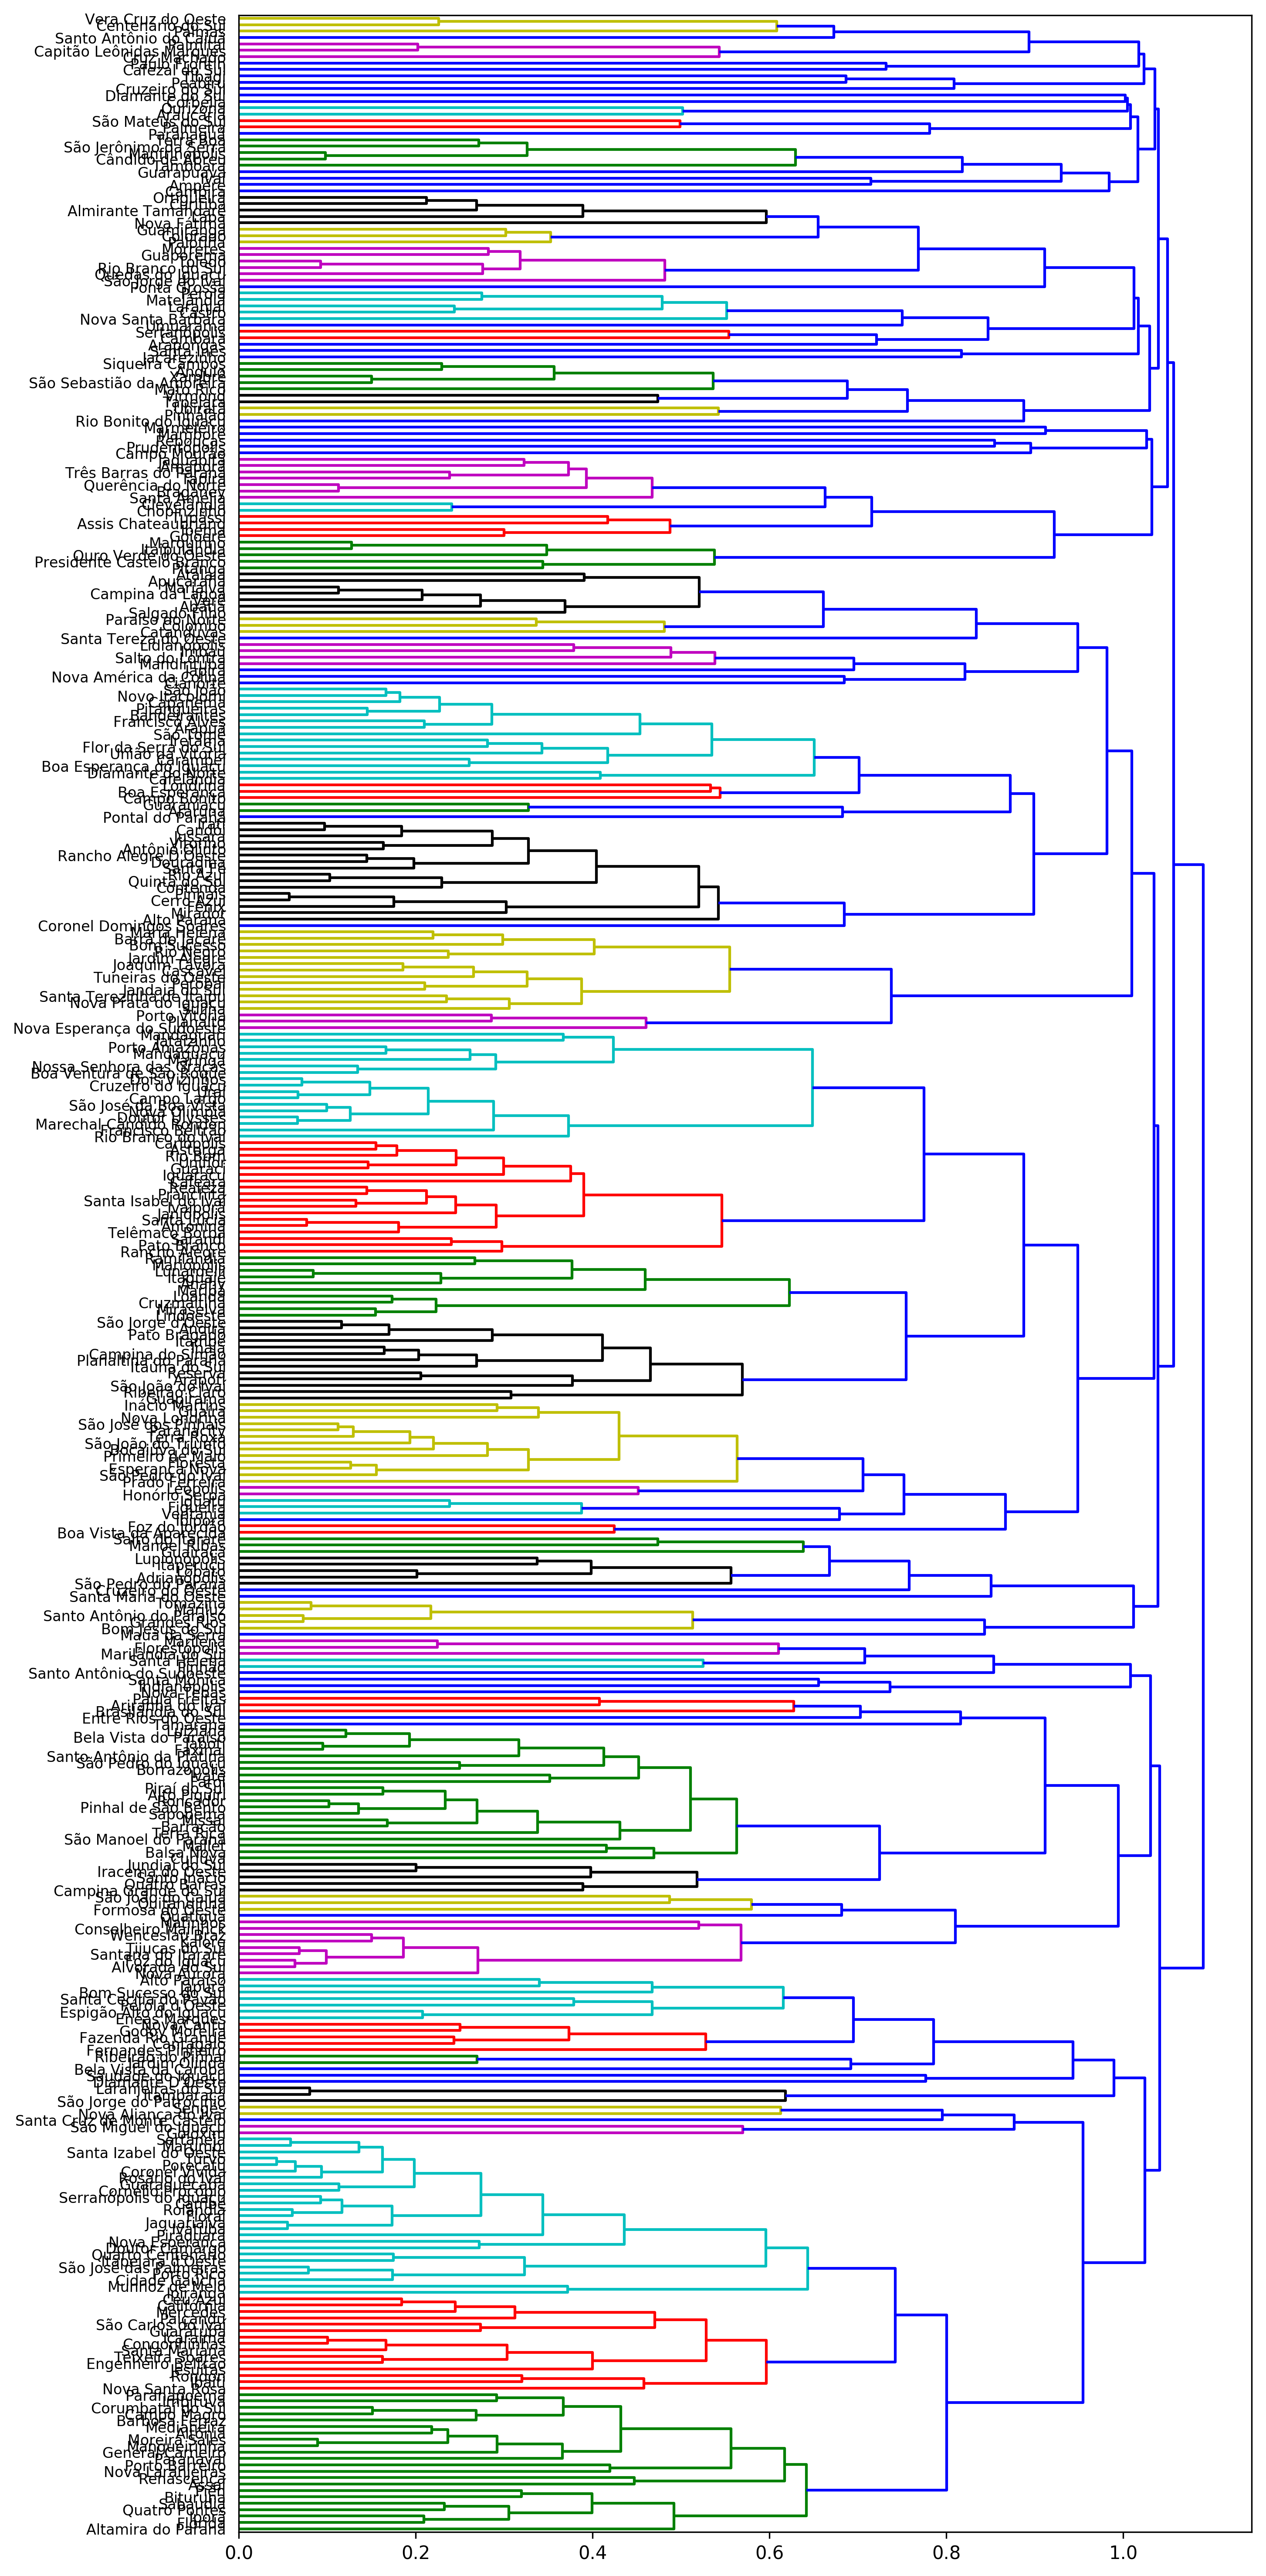
\includegraphics[height=\textheight]{clusterPR_06.png}
 % clusterRJ_0.6.png: 5971x2894 px, 300dpi, 50.55x24.50 cm, bb=0 0 1433 695
 \caption{Hierarchical cluster of Paraná.}
 \label{fig:cluster_pr}
\end{figure}

\begin{figure}[h!]
 \centering
 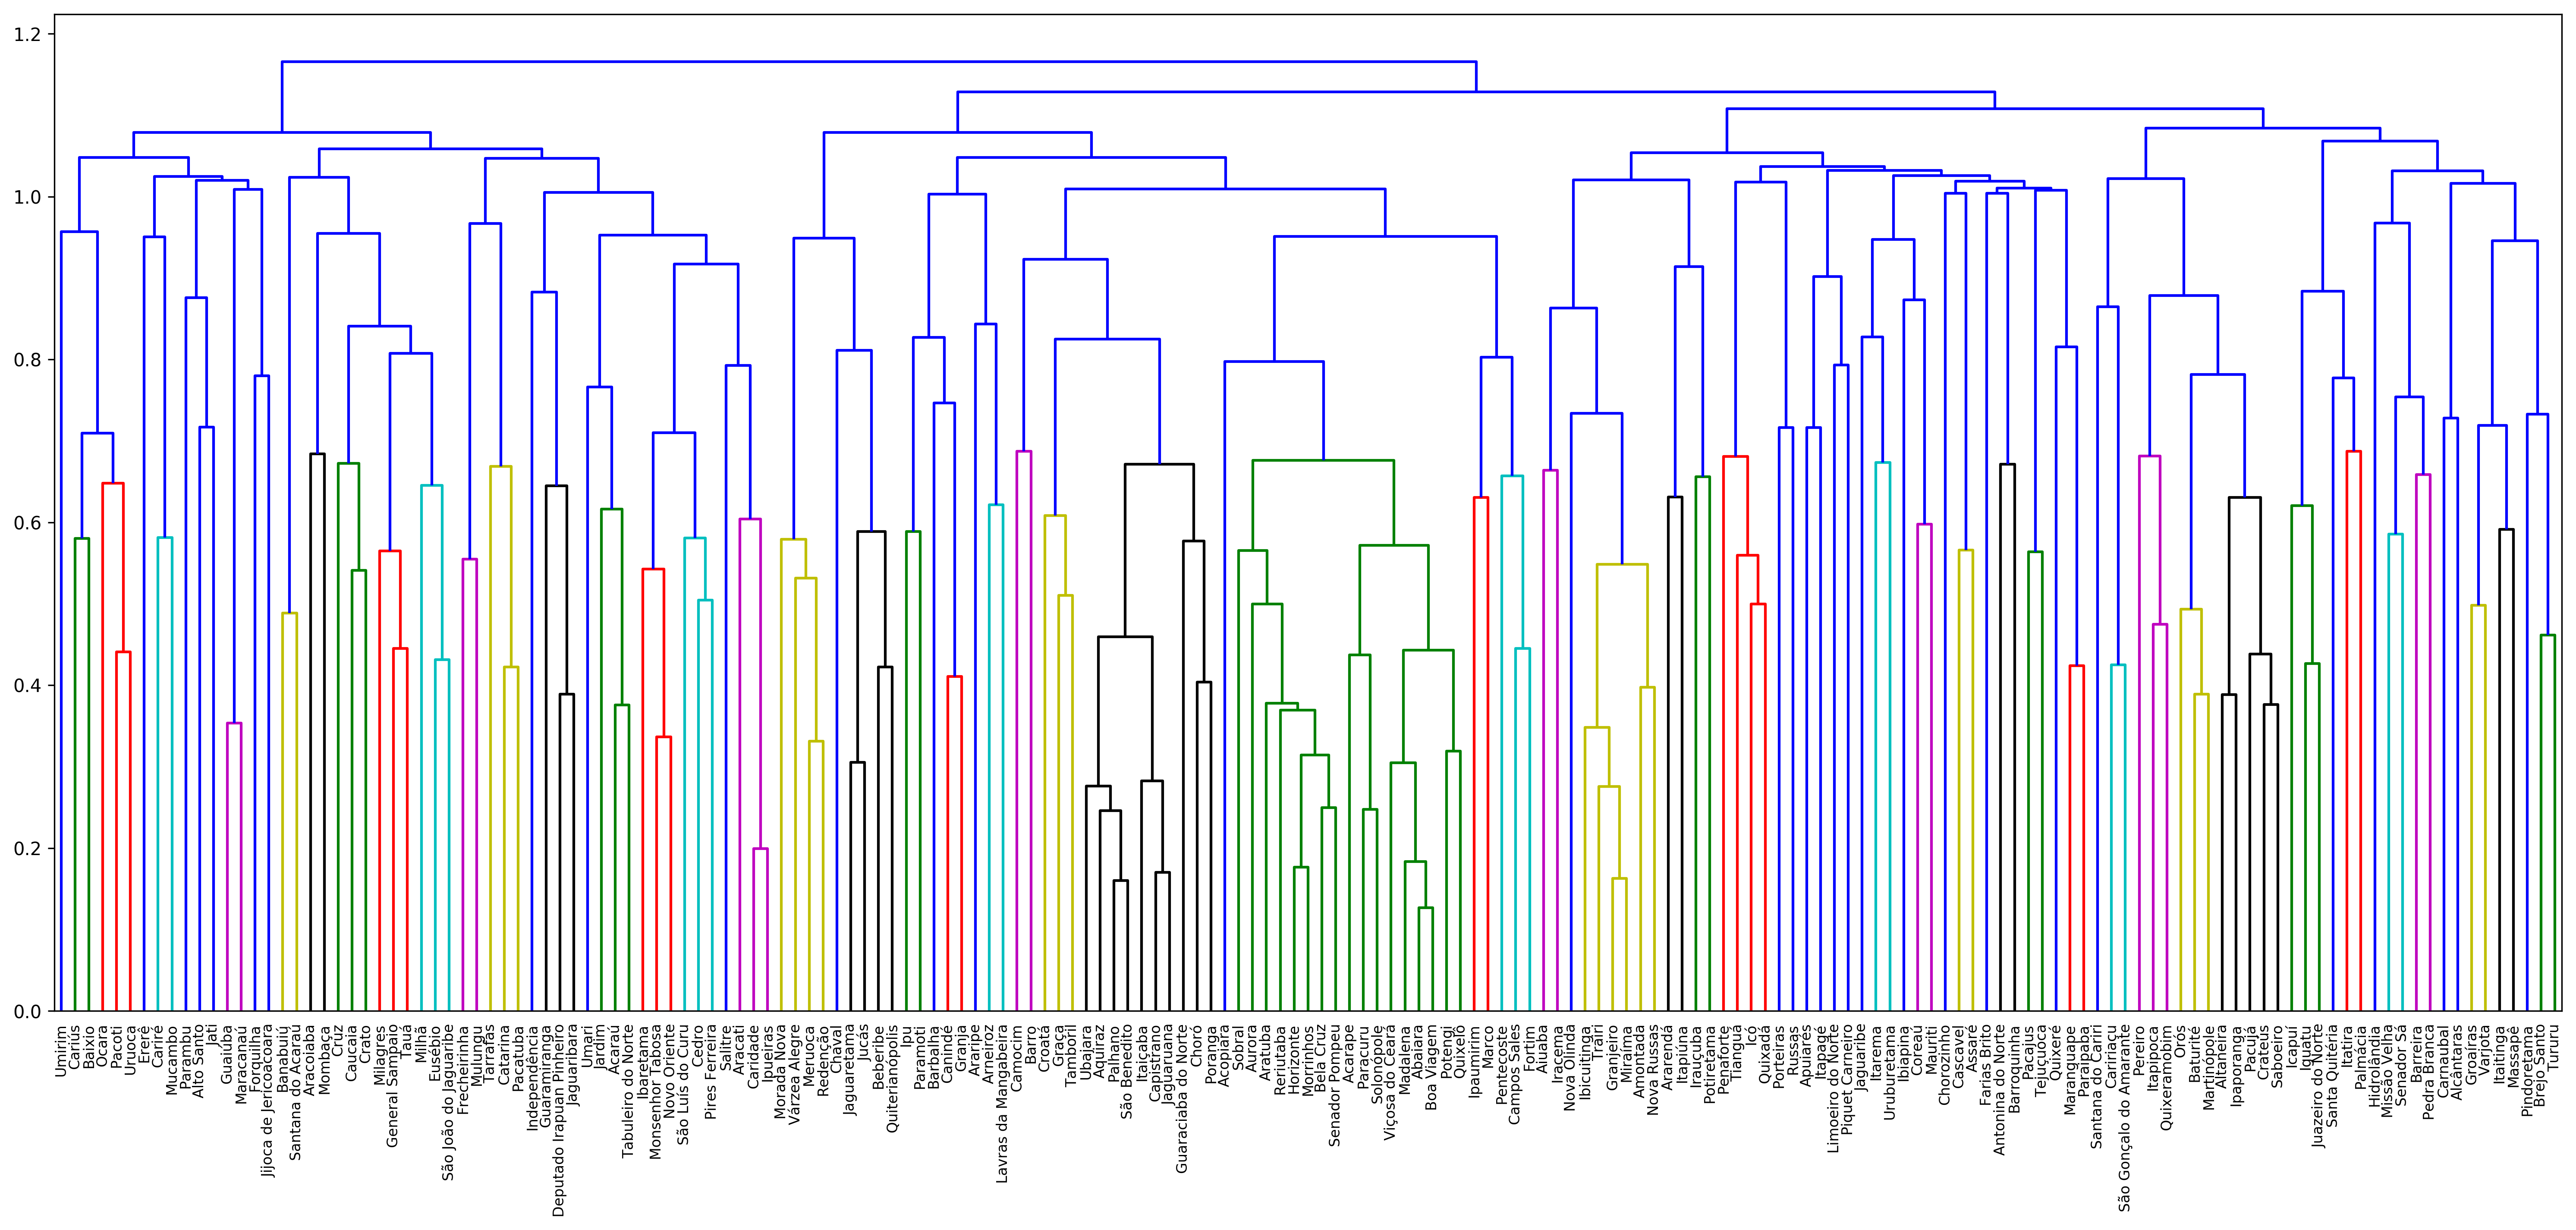
\includegraphics[width=\textwidth]{clusterCE_06.png}
 % clusterRJ_0.6.png: 5971x2894 px, 300dpi, 50.55x24.50 cm, bb=0 0 1433 695
 \caption{Hierarchical cluster of Ceará.}
 \label{fig:cluster_ce}
\end{figure}

\end{document}
